
\documentclass[master]{thesis-uestc}

\title{基于多尺度特征融合的边缘识别算法}{The Edge Detection Algorithm Based On Multi-level Representations}

\author{周峙龙}{Zhilong Zhou}
\advisor{高联丽\chinesespace 教授}{Dr. Lianli Gao}
\school{计算机科学与工程学院}{School of Computer Science and Engineering}
\major{计算机科学与技术}{Computer Science and Technology}
\studentnumber{201821080608}



% \author{***}{***}
% \advisor{***}{***}
% \school{***}{***}
% \major{计算机科学与技术}{Computer Science and Technology}
% \studentnumber{***}

\usepackage{tikz}
\usepackage{url} 
\begin{document}

\makecover
\originalitydeclaration
\begin{chineseabstract}
% 2014年AlexNet在ImageNet图片识别上的横空出世让人们认识到了深度学习的力量,最近几年,深度学习得到了快速的发展,并且已经广泛应用在了计算机视觉、自然语言处理、推荐系统和广告系统等领域,并且极大地推动相关领域的技术发展和革新。而基于深度学习的方法已经在相关领域的工业界得到了广泛的应用,并取得了良好的落地效果,我们本文主要聚焦于其中的计算机视觉领域这个大方向。在计算机视觉领域中,人们最开始研究的数据都是图片数据,基于这些在图片上的方法,人们逐渐蒋图片上的方法迁移到视频领域,并且根据视频领域特有的时序性等其他性质衍生出了后来的视频处理算法,图片的处理算法的研究仍然是计算机视觉研究领域的关键和基础。

图片理解的问题一直是计算机视觉领域的关键性问题,最近随着深度学习引领的计算机视觉的快速发展,相关的图片语义理解任务变得愈发关键。而边缘检测作为图片语义理解的基础任务,也得到了越来越多的关注。在传统的计算机视觉理论中,通过边缘的识别和检测,能够得到后续的图片分割等结果;而在深度学习时代,边缘检测和识别能得到后续的图片分割结果,并且在相关的图片分割、物体检测等领域,也能达到优化相关高层次任务效果的作用。边缘检测的任务定义是给定一张图片,我们对于图片上的每一个像素点,对其判断是边缘点还是非边缘点,也就是说,算法需要对图片上的每个像素都获得一个对应的分类,我们也可以把相关问题称为一个稠密预测问题,而对应的来说,边缘检测就是稠密预测里的二分类。而相关的稠密预测问题的难度和输入图片的分辨率成正相关,随着人类社会的发展,相关图片的分辨率变得越来越大,这也给边缘检测任务提出了更好的要求。

经过调研之前的边缘检测算法,其中的核心难点和改进点大致可以总结为一下几点:

1.算法缺乏对物体整体信息的捕捉,导致对于大物体的边缘识别效果不好。

2.神经网络中多尺度特征没有得到很好的利用,使得小物体和大物体的整体识别能力都受到了一定的影响。


为了解决上面的问题,本文提出了不同的解决方案来解决上述问题: 

1.为了对整体信息进行建模捕捉,本文引入了膨胀卷积的概念来提高网络对于整体信息的建模能力。 

2.为了更好的结合网络中的浅层和高层特征,本文尝试了不同的网络结构,并且最终得到了一个自顶向下和自底向上的双向的网络结构。

3.为了更好的捕捉多尺度的特征从而提高整体网络对小物体和大物体的整体感知能力,本文提出了金字塔上下文特征增强模块来捕获有不同感受野的特征。 

4.考虑到多尺度特征之间同时存在互补和冲突,为了在算法进行中动态的对特征进行筛选和过滤,本文引入了相关的注意力机制来对网络传输过程中的特征进行重组和过滤。

概括来说,本文经过不断实验尝试,提出了一个针对图片进行快速边缘检测识别的网络,给定一个输入RGB图片,算法能够快速得到对应的边缘识别结果图。论文选取了受研究人员们广泛认可的标准数据集BSDS500和NYUDv2进行实验,实验结果表明本问题提出的模型在相关评测指标下均达到了当前业界的最优性能,相关的网络结构具有延展性,可供后续的相同类型任务继续使用。

\chinesekeyword{边缘检测,深度学习,稠密预测,多尺度特征,注意力机制}
\end{chineseabstract}

\begin{englishabstract}
    Image understanding has always been a key problem in the field of computer vision. Recently, with the rapid development of computer vision led by deep learning, the related task of image  understanding has become increasingly critical. As the basic task of image understanding, edge detection has been paid more and more attention. In the traditional computer vision theory, through the edge recognition and detection, it can obtain the follow-up image segmentation results. In deep learning, edge detection can get the follow-up image segmentation results, and in the related image segmentation, object detection and other fields, it can also optimize the effect of related high-level tasks. The task definition of edge detection is given an image,  judging whether each pixel in the image is edge or non-edge, that is, the algorithm needs to obtain a corresponding classification for each pixel in the image, this problem can also call a dense prediction problem, and correspondingly, edge detection is in dense prediction. Classification. With the development of human society, the resolution of relevant images becomes larger and larger, which also puts forward better requirements for edge detection tasks.

    After investigation and survey, the core difficulties and improvement points of the edge detection algorithm can be summarized as follows:
    
    1.The algorithm lacks of the ability to capture the whole information of the object, which leads to the bad effect of edge recognition for large objects.
    
    2.The multi-scale features in neural networks are not well investigated, which affects the overall recognition ability of small and large objects.
    
    In order to solve the above problems, this thesis proposes different solutions to solve the above problems as follows:
    
    1.In order to capture the whole information, this thesis introduces the concept of expanding convolution to improve the modeling ability of the network.
    
    2.In order to combine the shallow and high-level characteristics of the network better, this thesis tries different network structures, and finally obtains a top-down and bottom-up bidirectional network structure.
    
    3.In order to capture multi-scale features better and improve the overall perception ability of the whole network to multi-scale objects, this thesis proposes a pyramid context feature enhancement module to capture features with different receptive fields.
    
    4.Considering the complementarity and conflict between multi-scale features, in order to dynamically filter the features in the process of the algorithm, this thesis employs an attention mechanism to reweight and filter the features in the network transmission process.
    
    In summary, this thesis proposes a network for fast edge detection of images after continuous experiments. Given an input RGB image, the algorithm can quickly get the corresponding edge detection result. In this thesis, BSDS500 dataset and NYUDv2 dataset, which are widely recognized by researchers, are selected for experiments. The experimental results show that the proposed model achieves the best performance in the current industry under the relevant evaluation metrics, and the network structure has scalability, which can be used for subsequent tasks of the same type.

\englishkeyword{Edge Detection, Deep Learning, Dense Prediction, Multi-scale Features, Attention Mechanism}
\end{englishabstract}

\thesistableofcontents

\thesischapterexordium

\section{研究工作的背景与意义}
% 最近随着互联网时代的来临,甚至移动互联网时代的到来,使得互联网这一当时新兴的概念已经风靡全球,引领了新时代信息社会的发展。伴随着互联网时代的来临,应运而生的是人们在互联网上进行交互的海量数据。海量数据的处理推动了大数据技术的发展,机器学习作为大数据时代的标志性方法 ,也在大数据时代得到了长足的发展和广泛的应用。可以说,机器学习、数据挖掘等海量样本的挖掘分析方法,已经对人类现代社会产生了巨大的变革和影响。

机器学习,顾名思义,可以通过对大数据样本的分析和挖掘使得机器能够自动学习,学习海量数据中蕴含的知识并将这种知识利用在其他的相关领域。在机器学习之后,人们基于机器学习的思想思考出了一种新的自动学习方式叫做深度学习。
% 深度学习的灵感来源于人类大脑的学习方式,通过模仿人类神经系统中一层一层的神经元和神经末梢对于信息的传递过程来对海洋样本的数据进行模式和知识的学习。在人脑的神经系统中,神经元会接受传递而来的电信号,并且对整个神经元接受到的电信号做一次计算和规整来判动作点位信息的产生,根据相关的动作电位信息,将相关信息传入进入神经末梢进而传递到下一层神经元。而深度学习的学习模式和上述描述几乎相同,深度学习接受的信息通常是图片、视频、文本、语音、其他结构化和非结构化数据,并且通过多层神经元和多层激活层的连续处理对相关的数据数据提取其中深层蕴含的信息,得到相关的数据编码即数据特征。 
相比于传统的机器学习和传统的大数据分析方法,深度学习能够通过人工神经网络对数据高层和浅层特征信息的获取替代之前人们常用的手工制作特征,而这种自动提取出的特征相对比手工特征有个更丰富的语义信息和对数据全局的理解能力,因此能够取得相对于手工特征更好的效果。

最有标志性的时间是2014年AlexNet\citing{AlexNet}在ImageNet\citing{ImageNet}图片识别上的横空出世让人们认识到了深度学习的力量,也引爆了最近相关领域的深度学习研究。最近几年,在全世界各个领域研究者的努力下,深度学习得到了快速的发展,并且已经广泛应用在了计算机视觉\citing{kaiming_deeplearning, DensePose}、自然语言处理\citing{nlp}、语音、推荐系统和广告系统等领域,并且极大地推动相关领域的技术发展和革新。而基于深度学习的方法已经在相关领域的工业界得到了广泛的应用,并取得了良好的落地效果。在计算机视觉领域中,人们最开始研究的数据都是图片数据,基于这些在图片上的方法,人们逐渐蒋图片上的方法迁移到视频领域,并且根据视频领域特有的时序性等其他性质衍生出了后来的视频处理算法,图片的处理算法的研究仍然是计算机视觉研究领域的关键和基础。而在自然语言处理领域,人们能够通过深度学习的技术和模型对任意输入的文本得到其代表的语言特征,让机器理解文本所代表的含义,同时也可以通过神经网络对文本进行翻译转换,得到人们想要的语言文字。在语音领域,深度学习算法能够对输入的语音数据进行处理和分析,得到对应的语音理解结果保存在特征中,这些特征可以用于后续的相关处理。包括现在逐渐进入人们生活的智能音箱中的语音语义理解和对话问题,背后都有着深度学习相关技术的支撑。在推荐系统和广告系统领域,相关基于深度学习的技术数不胜出,并且发表了许多卓有成效的顶级会议期刊论文,并且已经在顶级互联网公司的实际系统中落地带来了良好的效果收益。深度学习的应用还能够在这些领域跨领域的使用,得到人们定义的各种问题的解决方案,例如结合计算机视觉和自然语义处理,我们可以对输入图片生成对应的文字描述,同样也可以对输入文本生成对应文本描述的场景图片;结合语音和计算机视觉技术,我们能够利用输入的语音驱动任务说话等等。我们可以发现深度学习催生了很多有趣并且有利用价值的应用,并且在传统的领域也能达到令人惊艳的效果。

我们本文主要的关注点在计算机视觉领域。计算机视觉主要是研究机器对于视觉的感知能力,赋予机器对于图片、视频等视觉模态进行自动化的分析的能力,需要和另一大研究领域计算机图形学作出一个明显的区分和分别,计算机图形学的主要研究内容是研究如何在计算机中表示图形、以及利用计算机进行图形的计算、处理和显示的相关原理与算法。其中主要的几大研究内容包括图片/视频识别、分割、检测等任务,在这些基本任务的基础上还能引出很多计算机视觉的细分任务。例如分割任务可以分解为语义分割、实例分割和全景分割等多种细节任务任务。而图片识别又可以分为图片识别和图片的细粒度识别。

在这些任务之中,图片识别任务是最基础的一个基石性任务,后续计算机视觉很多的任务主干都会利用图片识别任务的网络模型,之后在具体任务上进行自定义的调优和训练。本文研究的内容是边缘检测识别任务,并且针对的数据对象是图片数据,相对于图像分割和检测任务,边缘检测任务是已给相对较低层次的任务,可以为上游的相关任务提供更多的信息达到辅助上游任务表现的效果,同时也可以单独的作为系统中的一个模块用于对整体环境和数据进行场景化的理解。任务的定义是给定一张RGB图片,算法需要对于给定图片中的每一个像素,判断其是否是属于边缘的像素点。其中常规认知里,我们认为边缘是图片中局部灰度变化较为剧烈的地方,所以我们可以定义边缘为图像中发生灰度值剧烈变化情况下的区域边界点。

细致分析这个任务定义,我们可以得到一些任务的特征:边缘检测任务是一个对于每个像素都需要进行分类的一个稠密分类任务,且是一个稠密的二分类任务;边缘检测输入图片中每一个像素可以看成一个需要分类的样本,对于给定的任意一张图片,在正常情况下,图片中边缘点的个数一定是远远小于非边缘点个数的,即给定数据中正样本的数目一定远远小于负样本数目,有着显著的数据不平衡的问题;边缘检测算法的难度随着场景复杂度和图片分辨率的有着正相关的关系。基于上面所述的这些任务特征,我们需要在设计算法的过程中充分考虑才能达到一个良好的效果。

虽然边缘检测这个任务在传统计算机视觉里已经有了很悠久的历史,最近几十年许多的研究者在上面花费了自己的心血,创造性的提出了各种新颖而有效的算法,有利用手工特征打造的边缘检测算法和利用新兴深度学习方法得到的边缘检测算法,但是这样的任务在深度学习时代仍然有着一些问题和一些可以提高的地方,主要原因就是随着移动互联网时代的兴起,人们日常浏览的图片和视频清晰度越来越高,室外的自然场景越来越复杂,而人们日常生活中的使用设备渐渐从电脑主机端移动到了智能手机端,对算法的运行效率和效果提出了更大的考验。而现在的边缘检测算法,很难做到对复杂的、包含不同大小物体的室外场景得到有效精细的边缘检测结果。所以边缘检测仍然具备极大的商业价值、社会价值和研究价值。

边缘检测的研究价值引导我们分析现在主流的边缘检测算法,并且提出满足要求的新算法从而达到社会发展的要求;同时我们也能利用边缘检测算法得到的结果用于弱监督学习和半监督学习中提供初始分析或者修正初始结果;同时也能基于边缘约束地学习其他目标,比如为了分割清楚边缘,把一个任务和边缘一起训练,这类的研究也取得了一定的成效\citing{segmentation_edge}\citing{saliency_edge}\citing{saliency_edge2},有助于解决分割算法中分割结果边缘不精细的问题了;同时也能利用快速的边缘检测算法转化为超像素用于任务的后处理。而其中正负样本极其不平衡的问题也值得我们针对这样一个特性提出更有效的方法来解决这个问题。

其商业价值在与如果我们能够快速得到的给定图片的边缘图,我们能够通过得到的边缘图对复杂环境下的设备进行监控。其中边缘检测算法已经被用于国内最大的风电设备企业,用于对复杂环境下价值上千万元的风力发电机设备的监控,节省了极大的财力物力。而边缘检测算法能够辅助后续的图片理解任务达到一个新的台阶,现在人们越来越感受到辅助驾驶甚至自动驾驶是未来科技的一个发展方向,在现今火热的自动驾驶技术中,相关的车道线检测技术、无人车的内感知系统中的分割和检测也能通过边缘检测得到更好的修正。

总而言之,图片边缘检测和识别是一个十分值得研究的课题,它是后续图片理解任务的基础,能够辅助后续的图片理解任务达到更好的效果,最终实现图像上的高层的语义理解,是模式识别、图像理解和分析、计算机视觉领域的基本步骤和关键方法之一。而且它在现今社会快速发展的要求下,有个更严格的精度和速度要求,并且仍然存在很多问题值得我们去进一步探索和研究,对边缘检测的研究和探索是具有十分长远的意义。

% \footnote{脚注序号“\ding{172},……,\ding{180}”的字体是“正文”,不是“上标”,序号与脚注内容文字之间空1个半角字符,脚注的段落格式为:单倍行距,段前空0磅,段后空0磅,悬挂缩进1.5字符;中文用宋体,字号为小五号,英文和数字用Times New Roman字体,字号为9磅;中英文混排时,所有标点符号(例如逗号“,”、括号“()”等)一律使用中文输入状态下的标点符号,但小数点采用英文状态下的样式“.”。}


\section{边缘检测算法的国内外研究历史与现状}
边缘检测算法的研究最早要追溯到上世纪60、70年代,在传统的计算机视觉任务中,边缘检测任务是通过一个叫做滤波的操作完成了。实际上,边缘检测就是一种滤波算法,而不同滤波的效果取决于对于滤波器的选择上。基于这个滤波的概念,深度学习的研究者们研究出了各种各样基于滤波的边缘检测算法,取得了不错的效果,并且能够达到实时的处理速度。一些著名方法\citing{Canny}的相关工具甚至已经被内置在Matlab工具箱中,供使用者直接调用。

对于传统的边缘检测方法,有一类基于特征学习的方法比如Pb\citing{Pb},gPb\citing{gPB}和SE\citing{traditional_1},他们通过采用通常复杂的学习范式根据局部的低层次的特征(例如灰度强度、梯度和纹理)来,获取对应的边缘强度\citing{traditional_6}。还有一类更为常用的是是使用相关的边缘检测算子来计算图片上每个点在横向和纵向方向上的梯度值,梯度值在数学中可以表示函数在某点处值的变化情况,这里通过梯度能够得到图片在每一个点上灰度在x和y方向上的变化剧烈情况,从而得到基于滤波的边缘检测结果。传统的边缘检测算子有Roberts边缘检测算子、Sobel算子、Prewitt边缘检测算子、Laplace边缘检测算子和Canny边缘检测算子\citing{Canny}。他们的差距主要在于滤波模版的大小和元素值不同,又可以区分为一阶的滤波算子和二阶的滤波算子。这些边缘检测算法主要有以下几个流程:

1)利用高斯滤波对图片进行过滤去除图片中多余的噪声,这一步非常重要,防止噪声对图片边缘检测的影响。因为噪声在图片中通常会造成局部的剧烈灰度变化,最后会被识别为边缘,造成错误识别。

2)利用相关的边缘检测算子对图片进行滤波,获取图片在两个方向上的梯度值和梯度方向。

3)对滤波得到的梯度值做非极大值抑制和阈值处理等后处理,得到对应的边缘检测结果图。

这些传统计算机视觉领域的边缘检测方法能够在一些简单的场景中取得还不错的精度和速度,但是手工制作的特征犹豫缺乏高层次的语义信息,导致传统方法在面对复杂场景上的效果很差。通过后续的发展我们可以看到,深度学习方法的效果在不同场景下均远远超过了传统视觉的检测方法。

最近,随着深度学习的发展,卷积神经网络模型已经称为了提高大多数计算机视觉任务效果的一个最流行的方法了,例如在图片识别(Image Classification)\citing{Inception}\citing{Inception2}、目标检测(Object Detection)\citing{FPN}\citing{FasterRCNN}、语义分割(Semantic Segmentation)\citing{FCN}\citing{PSPNet}、视觉问答(Question Answering)\citing{vqa1}\citing{vqa2}和图片字幕生成(Image Captioning)\citing{Captioning}\citing{Captioning2}等任务中,卷积神经网络都已经取得了十分突出的效果。在一些以前的工作中[引用]已经展示了端对端训练好的深度卷积神经网络相比于之前基于手工制作特征的方法,在很多高层次(high-level)的计算机视觉任务中有着显著的提高。在深度神经网络在许多计算机视觉任务上都取得良好效果的情况下,也有研究者开始研究深度卷积神经网络能够在低层次(low-level)的计算机视觉任务中也取得良好的效果,而边缘检测就是其中一个低层次的计算机视觉任务。在这个背景下,研究人员提出了很多深度学习的边缘检测器。

在早期的深度学习方法中,主要通过卷积神经网络提取图片的高层次语义特征用于对边缘进行检测和提取。Bertasius等人提出了DeepEdge\citing{DeepEdge}的方法,这是一个统一的多尺度深度学习方法。它首先利用Canny边缘检测算子去提取候选的边缘点,之后通过它的深度神经网络KNet提取图片的高层特征。这个方法的网络有两个分支,一个分支用于回归得到边缘点,一个分支用于分类得到边缘点。最后通过全连接层,训练好的DeepEdge模型能够能够对于一个固定尺寸的图片输入,得到对应的边缘点图片。Ganin等人提出了N$^4$-Fields\citing{N4_Field}方法,它结合了深度神经网络和最近近邻搜索从而得到边缘检测的结果。Shen等人提出了DeepContour\citing{DeepContour},其中把边缘数据划分为几个不同的子类,并且使用模型参数拟合的方法去对每一个子类进行学习从而得到最终的结果。

Xie等人提出了HED\citing{HED}这一个工作,这是深度学习时代第一个实现端对端训练和预测的边缘检测算法。所谓端对端,是指网络输入一个图片,网络能够直接在输出得到一个对应的结果,所有的算法处理都在网络中自动完成,没有其他中间过程和模块。端对端相比于之前的深度学习方法保证了整个算法的运行速度和实用性。在HED结构中,将一个图片识别网络作为主干网络用于提取输入图片的特征,对于主干网络的每层输出,作者使用了卷积核尺寸为1的卷积层,一个反卷积层和一个Sigmoid激活函数层得到对应侧枝上的预测结果。并且通过一个“拼接加卷积”的方式将总共五层的侧枝输出合并在一起作为网络最后的预测结果输出,可以看作对多个侧枝的输出加权平均得到最终结果。HED方法相比之前的非端到端方法,取得了巨大的效果和速度的提升。同时这篇文章探索了很多利用深度学习去解决边缘检测问题时的常用策略,例如跳跃结构(Skip Connection)、深度监督(Deep Supervision)等,为后续深度学习时代的边缘检测做了开创性的贡献。Liu等人提出的方法Relax使用了非严格二值化的边缘标注作为真值去指导整个网络的训练,达到了更好的效果。Wang等人提出的CED方法利用了一个自顶向下的网络结构,从高层到底层逐渐优化边缘的思路达到了良好的效果,作者在网络中还利用了像素随机化(Pixel Shuffle)\citing{PixelShuffle}这一个在超分辨率领域使用的上采样方法来代替传统的双线性插值和反卷积的上采样方法,取得了不错的结果。Xu\citing{AMHNet}等人的工作提出略一个层次化的深度学习模型,并且利用条件随机场来鲁棒性地结合不同层次学习到的边缘特征表达,取得了良好的效果。这也证明了之前方法对于多层次特征表达的有效融合并没有进行一个很好的挖掘和探索,这也是我们一个主要探索的领域。除此之后 ,Yu等人提出的工作CASENet\citing{CASENet}还成功将边缘检测算法这个任务延伸到了语义边缘检测领域,其中对于每个像素点,不仅要判断其是否是边缘点,还需要对每个边缘点判断它的类别。不过这个任务暂时不在本文的研究范畴,只是在这里介绍相关算法的研究现状和扩展研究。Zheng等人提出的工作\citing{zheng2019differential}利用了生成对抗网络结合遗传算法去预测边缘。

作为图像理解中的一个基础步骤和重要模块,在基于深度学习的边缘检测中,多尺度特征的有效融合是一个很关键的、具有很高研究价值的研究课题。多尺度特征的有效融合在许多任务中也是一个基本的、关键的研究点。例如在Yan等人提出的关于行为识别的工作\citing{yan2018hierarchical}中,作者利用层次性的多尺度注意力网络充分挖掘了多层次特征融合的问题,并且得到了良好的效果。在Chen等人提出的工作中\citing{chen2016attention},对于语义分割这一个图像理解问题,多尺度特征融合策略的有效挖掘同样达到了满意的效果。挖掘多尺度的特征不仅可以通过浅层和深层神经网络来自然实现,同时也可以通过特征金字塔结构达到这个效果。在为了解决语义分割问题而提出的DeepLab\citing{DeepLab}和PSPNet\citing{PSPNet}中,作者都提出了利用特征金字塔结构来获取多尺度的特征,并将多尺度特征结合达到了当时最先进的结果。而在边缘检测领域,Xu等人提出的AMHNet\citing{AMHNet}对边缘多层次特征表达利用基于条件随机场的层次化网络结构进行融合,也达到了当时领先的结果,但是条件随机场会拖慢整体网络的推理速度,这也引导我们针对这个领域中的这一研究点进行更深入的研究。

基于上述所述的研究点,在边缘检测领域,我们仍然有很长的路要走,有很多方法和模式需要挖掘。现今基于深度学习的人工智能虽然已经在计算机视觉 甚至图片理解领域取得了很大的成功,但是距离我们想象中的强人工智能还有很长一段路要走。正如上述所说,实现快速和精准的边缘检测对于图片像素级别的理解是最基础的一步,这将有利于我们实现真正意义上的图像理解。

\section{本文的主要贡献与创新}
本文研究的领域是计算机视觉领域中的边缘检测算法。针对边缘检测方法中现在存在的一些问题,本文关注在边缘检测中的多尺度特征融合问题上。本文的主要贡献和创新点如下:

1)在边缘检测领域,之前的方法缺乏对输入图片全局信息的获取能力,本文引入了膨胀卷积的模块,在保证网络中特征图大小不变的情况下提高了特征图的感受野,用于捕获图片的上下文语义信息。

2)为了赋予网络感知多尺度输入图片和多尺度目标的能力,我们在网络中引入了特征金字塔的结构。其中金字塔结构由不同采样率的膨胀卷积构成。我们探索了分别将特征金字塔结构作用在主干网络的最后一层特征和主干网络提取的所有多尺度的特征上,都取得了良好的效果。

3)我们引入了注意力机制用于在特征传输过程中指导特征的传递,我们引入了空间和通道上的软注意力机制,将其应用在了自底向上和自顶向下的两种不同的网络架构中。

4) 基于上面的模块,本文先后提出了两种边缘检测算法的网络结构。第一种结构是基于自底向上的特征优化边缘检测算法,利用单向的侧枝网络对主干网络提取的特征进行逐层融合优化,并且在侧枝中引入了空间注意力机制。第二种结构是基于自底向上和自顶向下两种架构的双向特征优化网络,利用双向网络的架构促进特征信息在不同层间的流动,提高特征的层次性,并且在双向网络中引入了通道注意力机制,对特征不同通道进行重组和过滤。为了解决预测边缘粗宽的问题,本文同时引入了Dice损失函数用于训练网络。

5) 在两个被广泛使用的公开数据集BSDS500和NYUDv2上进行了大量的对比实验和消融实验。对比实验证明了我们提出的方法的先进性。而消融实验也对我们提出的网络的各个模块进行了细致的分析。


\section{本论文的结构安排}
本文章节的结构安排如下 :

在第一章我们重点介绍了 边缘检测任务的背景和意义,并且大致描述了边缘检测领域从古至今的主要发展,并结合对不同方法的调研,总结出了现今边缘检测方法可以改进的方向和它所面临的挑战。在最后直接提出了本文的出发点、具体创新点和贡献。

在第二章节我们将主要介绍边缘检测领域基础知识,包括边缘检测的具体任务定义、经典的传统边缘检测方法、简单的深度学习时代边缘检测方法。 在对重点方法进行细节讲述之后,我们会对具体的边缘检测算法进行一个梳理和分类,帮助读者理解古往今来的边缘检测算法发展,也更能够深刻理解本文工作的出发点和贡献。我们将在这一章将简单介绍深度学习网络主要使用的卷积神经网络主要部件和概念,包括卷积层、反卷积层和膨胀卷积等基本概念,并且介绍图像理解中重要的上采样模块。我们还会在这一章具体梳理相关注意力机制的发展,为我们后续模块的使用打下基础。

在第三章我们将提出了一个基于自底向上的累计优化的边缘检测算法模型。为了解决网络在理解复杂场景时对于全局信息和语义信息的需求,我们引入了膨胀卷积的概念,在保障特征图尺寸的情况下提高了网络在高层的感受野。考虑到多尺度多层次特征的融合这一主要研究点,我们进行了一些实验上的尝试,并且取得了不错的效果。我们引入了特征金字塔结构在主干网络的一层当作分割的输出头用于得到具有不同感受野大小的多尺度特征,并且将这个特征作为主干网络特征的补充参与后续的优化流程。除此之外,为了更好融合主干网络浅层和深层特征,我们尝试了一个自底向上的侧枝网络结构,并在其中加入了残差结构和注意力机制用于提高网络的整体表现。最后在两个广泛使用的标准化数据集上进行了大量实验,证明了我们方法的有效性。

在第四章中基于第三章的网络设计上的经验,我们结合自顶向下和自底向上两种不同 方向的优化方式,提出了一个端到端的边缘检测模型。这一章提出的网络模型在设计上解决了上述模型的一些问题,在设计时达到了保证模型参数量的同时保证效果。我们在这个网络中将特征金字塔模块设计在主干网络的每个侧枝网络中,更加丰富了输出的边缘特征表示,并且引入了新的损失函数来处理正负样本不平衡的问题。最后在两个广泛使用的标准化数据集上进行了大量实验,实验证明提出的方法在公开数据集上达到了当时 学术界的最高水平,证明了我们方法的先进性。

第五章我们对全文内容进行总结,并且根据我们在实验中的一些感悟和经验指出了相关问题,并且提出了这个研究工作未来的发展方向。

\chapter{边缘检测算法基础}
在第一章中我们简单介绍了边缘检测任务从开始到现在的一系列发展进程和脉络,并且我们介绍了边缘检测任务在学术界和工业界的关键作用,我们知道边缘检测是图像理解任务中的基本步骤和关键性任务。在本章节中,我们将简单介绍卷积神经网络的主要功能模块。我们还将介绍边缘检测任务的主要定义,并且从传统计算机视觉的手工特征方法到现今基于深度学习的方法梳理整个边缘检测算法发展的脉络,详细介绍其中的一些经典的方法。除此之外,我们还将通过研究者前辈们的一些经典工作介绍注意力机制的发展,并且介绍注意力机制提出时的出发点和作用。

\section{深度学习基础知识}
在本节中,我们将简单介绍深度学习的基本结构和模块。本节将主要介绍在我们方法中常用的卷积神经网络的基本模块包括卷积层、反卷积层和膨胀卷积等概念。

\subsection{卷积神经网络}
卷积神经网络是现今深度学习领域最主要的网络结构模块之一,除了卷积神经网络之外还有循环神经网络等概念,但是在我们的网络模块中并不会使用到,所以在这里就不做过多介绍。在卷积神经网络中我们常见的模块有卷积层、池化层,有时还会使用全接连层用于分类。除此之外,我们在网络中还会利用反卷积等概念,在这里也将做详细介绍。

卷积是一个之前常常出现在信号处理中的概念,它的数学表达式为:
\begin{equation}
    f(x) * g(x) = \int_{R} f(x)g(t - x)dx
\end{equation}

卷积层顾名思义,是卷积神经网络的核心部件,也是网络中主要的一个计算单元。我们在卷积神经网络中可以通过卷积运算对图像进行一定程度上的分析和特征处理,达到对图像的高层次语义理解能力。卷积神经网络相比之前的全连接神经网络,极大的减小了网络的计算量和参数量,但是仍然能够维持很好的效果。这些卷积网络的优点来自于它的两大性质:局部感知和参数共享。对于局部感知这个性质,我们可以知道卷积层主要是由多个同样大小的卷积核构成,这里的卷积核也可以类比之前传统图像处理中的滤波器的概念。通常情况下,卷积核的尺寸会远远小于输入图片或特征的尺寸,而且卷积核的个数能够控制卷积层输出的特征(features)的个数,通常来说卷积层中几个卷积核,输出的就有几个对应的特征图,局部感知的特性体现在,每个卷积核都会在输入的图片或者特征上按规定的步长进行滑动,并且每次滑动都会利用卷积核和图片的局部数值做一次局部的加权求和运算,得到一个输出的结果。可以发现卷积层只在输入的局部通过滑动的操作做局部的计算和感知,并且卷积核的个数和输出特征的个数对应,说明了一个输出的特征图只对应一个卷积核,特征图上的各个部门共享了一个卷积核 参数,这也体现了参数共享的特征。局部感知和参数共享这两个性质 能够大幅度降低网络的参数量。并且我们知道,在大参数量小数据量的情况下,对网络进行训练很容易发现拟合的现象,而卷积层带来的参数量的降低也有利于避免过拟合的现象。我们能够通过图\ref{conv}代表卷积层的具体运算。其中深色部分为当前卷积窗口的运算区域, 深色部分右下角数字为卷积核的值,中间部分为输入图片或特征的值,右侧对应深色部门是经过一次加权平均后对应位置的结构图。图\ref{conv}展示了两次卷积运算过程中的运算示意图,读者可以通过两张图进而联想到整个卷积运算的流程。\footnote{卷积运算示意图图例来自:\url{https://blog.csdn.net/wsLJQian/article/details/103144552}}

\begin{figure}[h]
    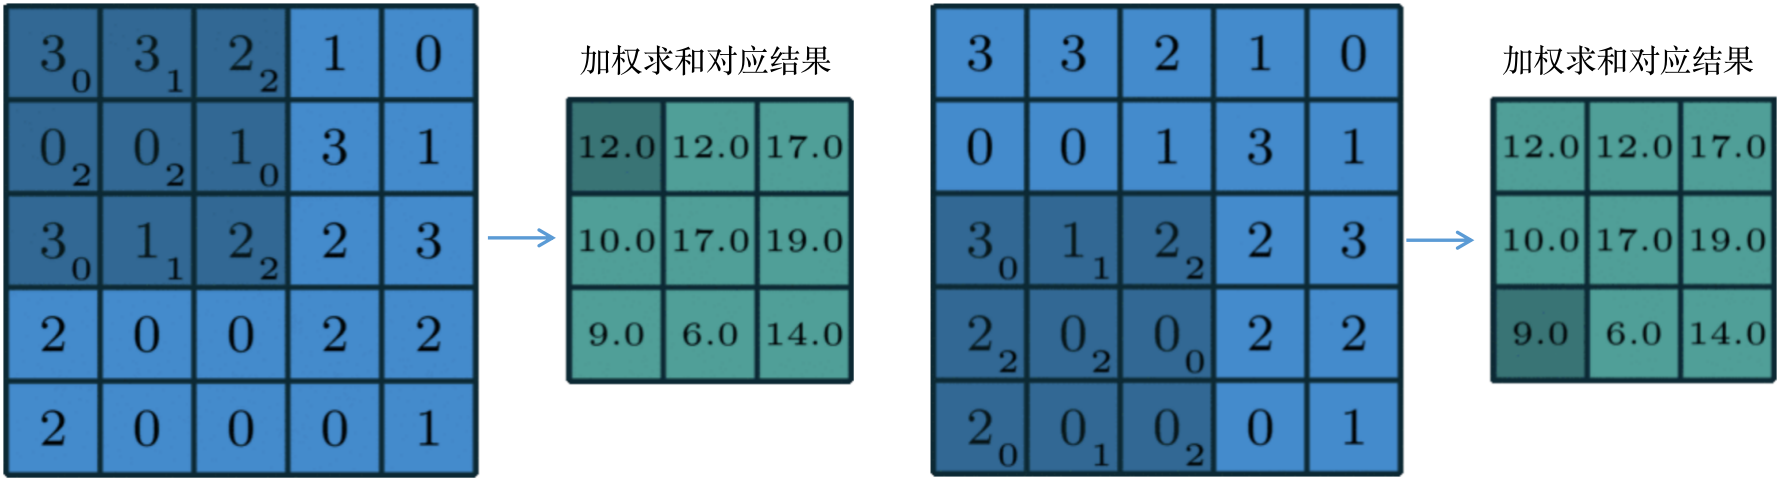
\includegraphics[width=0.75\textwidth]{convolultion.png}
    \caption{卷积运算示意图}
    \label{conv}
\end{figure}

我们也可以用数学表达式的方式表达图像中的卷积操作, 其中K代表卷积核的大小,y[i]卷积之后i位置的结果:
\begin{equation}
    \label{conv_equation}
	y[i] = \sum\nolimits_{k=1}^{K} x[i + k]w[k]
\end{equation}

激活函数层常常伴随着卷积层而出现,激活函数的作用是为整个神经网络添加非线性的能力。如果网络只存在卷积层,我们可以发现网络只是不断地在进行线性运算,整个网络所能表达的参数空间总是被限制在了一个 线性空间在中,这对整个网络的表达能力有着较大的限制。所以我们在网络中需要引入各种不同的激活函数。除了在神经网络中引入非线性能力这一点,有的特殊的激活函数还可以用于对网络的最后输出做限制,例如如果网络最后的需要一个0到1范围的输出,可以考虑使用Sigmoid激活函数来达到这一点。而在我们边缘检测任务中,就是这么做的。图\ref{activation}展示了几种常见的激活函数的示例。\footnote{激活函数图例来源为斯坦福计算机视觉公开课CS231n中的课程相关展示材料}其中不同的激活函数有不同的特点,例如Sigmoid可以讲值压缩在0到1之间,但是在输入数据过大过小的情况下容易出现梯度消失;ReLU是现今神经网络中最常用的激活函数,它解决了上述提到的梯度问题,但是在函数负半轴会损失一半的信息,这也引出了后续例如Leaky ReLU之类的激活函数的改进。


\begin{figure}[h]
    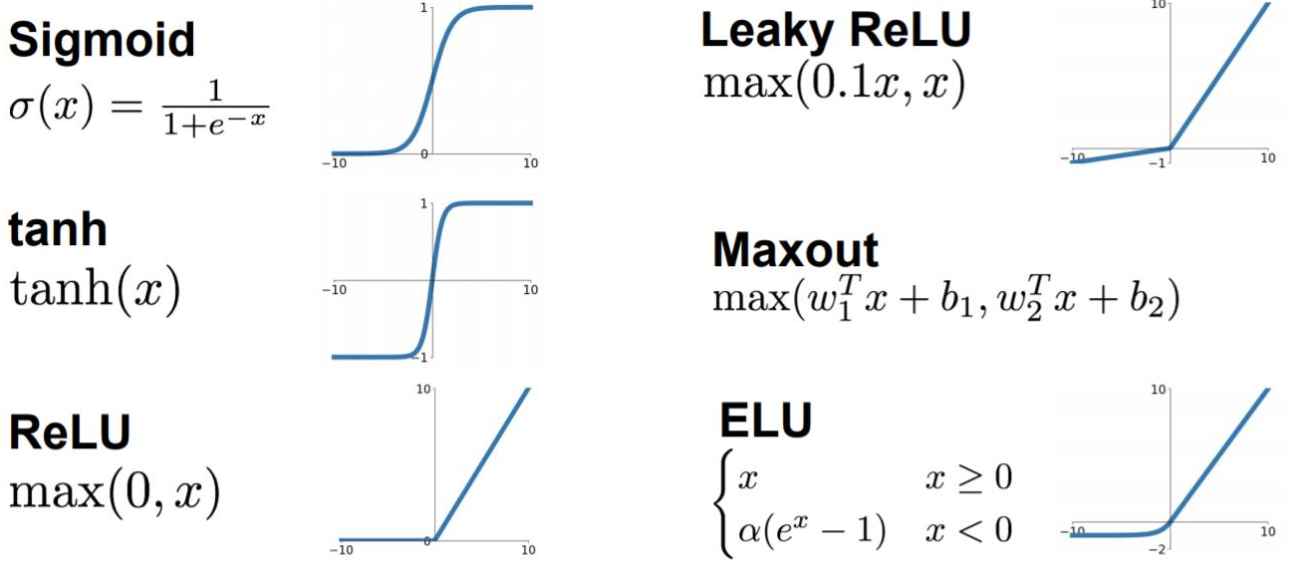
\includegraphics[width=0.95\textwidth]{activation_f.png}
    \caption{常见的几种激活函数示例}
    \label{activation}
\end{figure}

池化层也是经常出现在一个常规的卷积神经网络中。通过池化层能够使得网络中特征图的尺寸得到减小,可以使得网络后续的计算量逐渐减小。同时在图像理解领域,经过池化层计算后的特征图一般都具有较小的尺寸,但是能够具备较大的感受野。因为小尺寸上的每个一点都会对应输入图片的一大片区域,所以池化层的加入对于增大网络感受野也是非常有帮助的。同时,池化层具有的特征不变性使得网络的关注点从特征的定位变为了是否存在特征,可以容忍一定微小的位移。总而言之,池化层具有特征平移不变性、特征尺度缩减、过拟合等作用。常见的池化层有最大池化层、平均池化层等。 针对池化层的研究,也催生了后续各种对池化层的改进,包括动态池化层等技术,不在本文讨论范围之内。图\ref{pooling}展示了池化层的具体计算方式。\footnote{池化层的图例引用自斯坦福的计算机视觉课程CS231n中的课程相关展示材料}

\begin{figure}[h]
    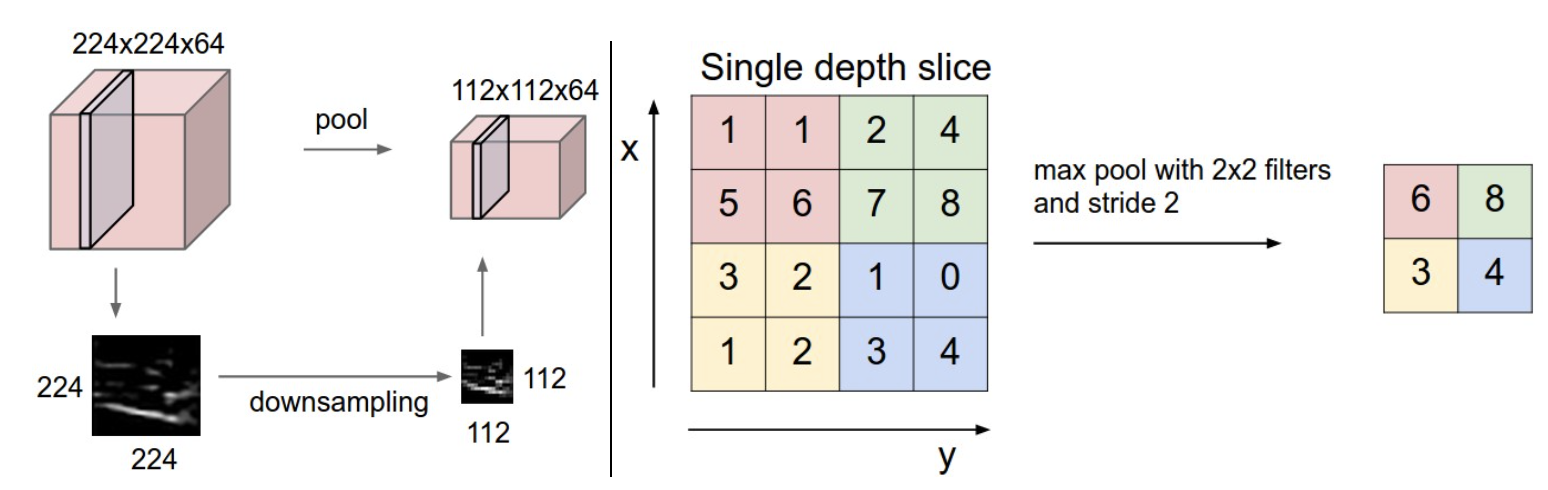
\includegraphics[width=0.95\textwidth]{pooling.png}
    \caption{池化层的计算方式图例}
    \label{pooling}
\end{figure}

全连接层在卷积神经网络中一般用于最后输出最后的特征嵌入结果,在现在的卷积神经网络中,通常被用作分类器。它能对输入的一个特征向量通过一个可以学习的参数映射到一个新的特征向量上。需要注意的是,在这种情况下,因为全连接层的参数需要作用到整个特征向量上,而在网络初始化阶段就需要设置好全连接层的参数维度,所以带有全连接层的神经网络只能接受固定尺寸的图片输出,无法接受任意尺寸的输入,这对稠密预测问题特别是边缘检测这个任务来说会造成一定问题,因为在输出最后对结果进行变化尺寸操作可能会造成畸变影响结果。 

在图像理解任务中,感受野的概念非常重要。在我们设计网络用于图像理解任务时,每层的感受野是一个很重要的指标。在生物学中,当响应到达是时,多层神经元将神经冲动传递到人的大脑中,才能让我们感受到刺激。感受野的感念是指一个对应的神经元所能感受和支配到刺激的区域。而在深度学习中,感受野通常是指某一层中的特征图中某一点的值,是由输入图片中一个面积为多少的区域计算出来的。即特征图上的每一个元素的计算和输入图像上某个多大的区域有关,这个区域的面积就是感受野的大小。 图\ref{respective_field}是感受野的一个图像表示。


\begin{figure}[h]
    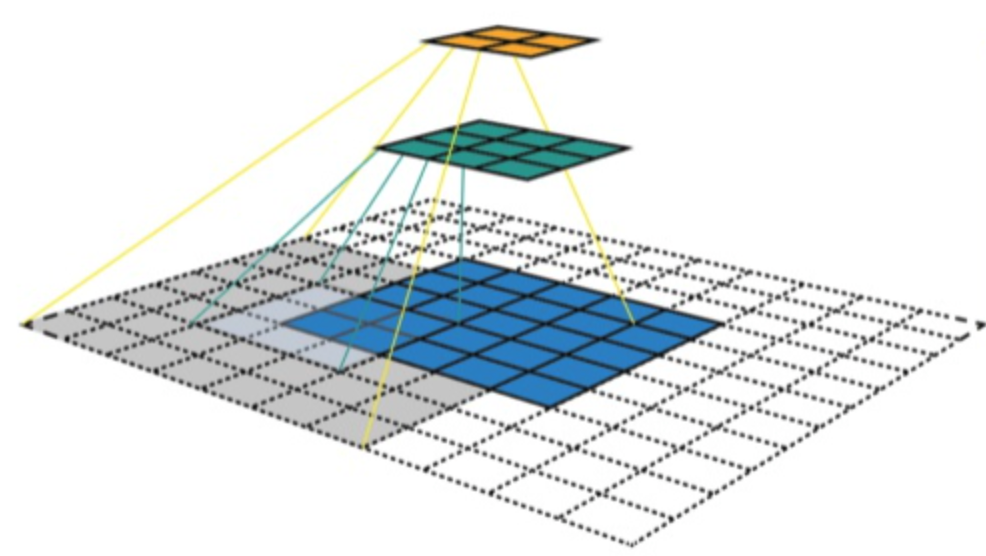
\includegraphics[width=0.55\textwidth]{respective_field2.png}
    \caption{感受野概念的图像表示}
    \label{respective_field}
\end{figure}

通过感受野的计算研究者们能够直观的了解该层神经元所能关注到的输入图像上的区域有多大。通常来说,一个拥有较大感受野的神经元能够获取图像的全局信息,获取更丰富的语义信息帮助网络对图像进行理解。


理论上来说,通过感受野的理论计算,只要我们堆叠足够的卷积层,高层的神经元就能获取输入图像的全局信息。例如VGGNet\citing{VGGNet}网络中,网络最后的理论感受野能到达196,能覆盖图像的大部分区域,看似没有增加网络深度从而获取更大感受野的必要性。不过最近几年有研究\citing{luo2017understanding}表明了网络中的有效感受野会小于通过计算得到的理论感受野大小。因为在计算得到的理论感受野中,每个像素对应于感受野的贡献并不相同,会随着感受野中心像素为中心呈高斯分布进行衰减,造成有效的感受野面积只有实际感受野面积的一部分。高斯分布中感受野边缘像素的贡献会随着卷积层的不断堆叠快速衰减,最后趋于一个可以忽略的极小值。图\ref{erf}展示了CIFAR 10数据集\citing{krizhevsky2009learning}进行图像分类任务和CamVid\citing{brostow2009semantic}上进行图像理解任务的实际感受野可视化,可见实际感受野呈高斯分布。

\begin{figure}[h]
    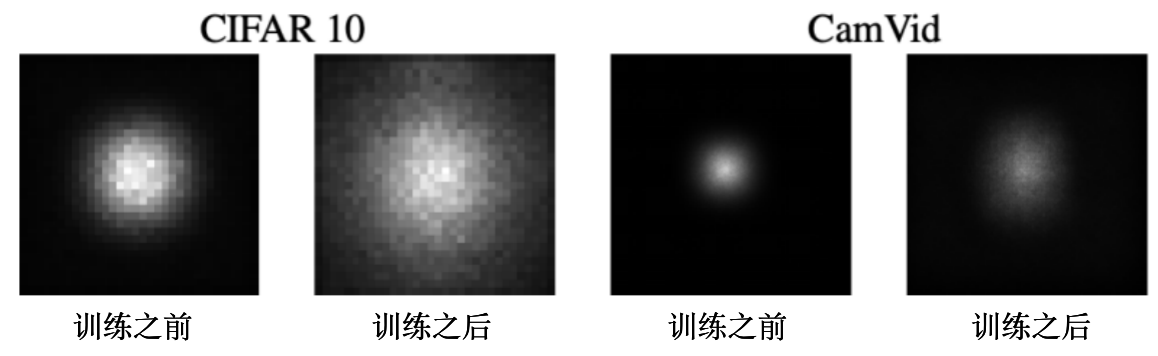
\includegraphics[width=1.0\textwidth]{ERF.png}
    \caption{实际感受野的可视化效果\citing{luo2017understanding}}
    \label{erf}
\end{figure}


从感受野的角度看待全连接层和卷积层,可以发现对单层来说卷积层的感受野只在对应卷积核大小的范围上,而对于全连接层来说,每一个输出的值能够覆盖整个输入的像素,所以也可以说全连接层能够一步获取输入特征的全局特征,所以十分消耗计算量。

卷积层、激活函数、池化层是卷积神经网络三个主要的构成模块它,有时需要分类的情况也需要加入全连接层,通过对这几种模块合理的设计和搭配,已经能够设计出效果比较好的卷积神经网络模型。但是为了对方法的进一步探索,我们还需要其他一些基础知识。

\subsection{上采样}
在图像理解领域,我们通常使用一个图像分类的主干网络用于提取图像上的特征,但是主干网络因为网络中不断的池化操作和步长大于1的卷积层的原因,特征图的尺寸会逐渐减少。但是图像理解作为一个像素级别的、稠密的预测任务,需要一个高分辨率的特征对结果作出一个精准的预测,所以网络中必不可少的一步就是对特征进行上采样,上采样到输入图片的大小。而上采样的大小也直接影响到最后稠密预测的准确度,特别是区域边界地区的精准度。在图像领域,上采样可以简单理解为从小分辨率到大分辨率输出的过程,如果把图像上的每个像素当作信号中的一个样本点,那么上采样的概念也可以和信号处理中的概念相对应上。常见的上采样操作包括有双线性差值(bilinear interpolation)、反卷积(deconvolution)\citing{deconvolution}和像素随机化(pixel shuffle)\citing{PixelShuffle}等。其中双线性差值是一种静态的上采样方法,而后两种是一种动态学习参数的上采样方式,不同网络中对上采样方式有不同的选择。

双线性插值因为其计算简单,不需要过多的额外参数,是使用最广泛的上采样方法之一。它的主要思想是假设平面上两个点之间的值都呈均匀分布,那么我们根据这个假设,就可以根据平面两个点的值,在x方向和y方向分别利用线性插值得到我们以两个点为顶点构成的矩形中任意一点的值。 类似的插值算法还有最近邻插值,即选取离目标点最近的点的值作为目标点的值,这个方法计算速度最快,但是效果不好;在实际应用中双线性插值是大多数情况下的默认插值方法。图\ref{bilinear}代表了双线性插值的示例。  在图\ref{bilinear}中,我们已知$Q_{11}$, $Q_{22}$点的坐标,可以推断出$Q_{12}$和$Q_{21}$点的坐标。我们目标点为$P \in (x, y)$,首先在x轴上进行双线性插值得到$P_{11}$和$P_{12}$,之后在y方向上通过线性插值得到最后的结果。我们把$Q_{12}$和$Q_{21}$一般化表示为$(x_1, y_1)$和$(x_2, y_2)$,可以得到如下表达式:
\begin{equation}
    f(P_{11}) =  \frac{x_2 - x }{x_2 - x_1} f(Q_{11})  + \frac{x - x_1 }{x_2 - x_1} f(Q_{21}) 
\end{equation}

\begin{equation}
    f(P_{12}) =  \frac{x_2 - x }{x_2 - x_1} f(Q_{12})  + \frac{x - x_1 }{x_2 - x_1} f(Q_{22}) 
\end{equation}

\begin{equation}
    f(P) =  \frac{y_2 - y }{y_2 - y_1} f(P_{11})  + \frac{y - y_1 }{y_2 - y_1} f(P_{12})
\end{equation}

\begin{figure}[h]\centering
    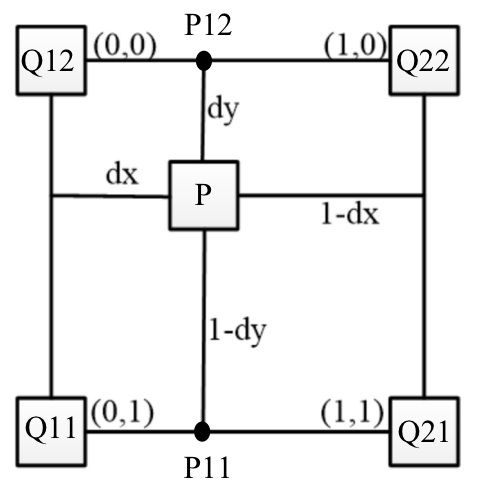
\includegraphics[width=0.35\textwidth]{bilinear_inter.png}
    \caption{双线性插值方法}
    \label{bilinear}
\end{figure}

双线性插值在卷积神经网络中可以单独出现,也可以搭配一个$1x1$的卷积层出现,卷积层的出现解决了双线性插值静态上采样的问题,可以把卷积层的参数理解为对应上采样的参数,可以通过网络动态学习得到,可以和后续的反卷积形成对比。

还有一种上采样方式为反卷积,是可以通过类似卷积操作达到上采样的效果。
反卷积其实更通用的叫法是叫转置卷积,因为反卷积容易让人和其他概念相混淆,它其实并不完全是反向的卷积过程。其实把它理解为卷积的转置矩阵更为合理。因为通过$Y = WX$,相反的操作就是$W^TY = X$。转置卷积的具体示意图为图\ref{deconv}。\footnote{反卷积相关的图例引用自斯坦福计算机视觉公开课CS231n的课程相关材料。}
\begin{figure}[h]
    \centering
    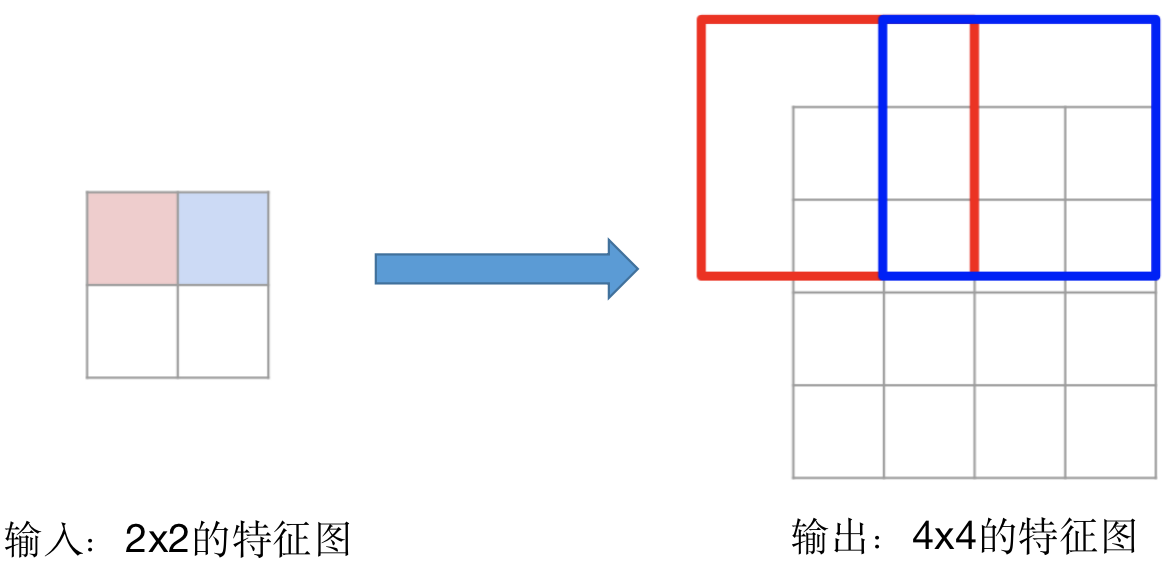
\includegraphics[width=0.5\textwidth]{deconvolution.png}
    \caption{反卷积的计算方式图例}
    \label{deconv}
\end{figure}

值得注意的是,如果在实际使用中,如果反卷积参数配置不正确,输出的对应特征图很容易出现棋盘效应, 如图\ref{grid_effect}所示。而另一种和反卷积能达到相似效果的方法是双线性插值之后通过一个卷积层。同样能达到改变上采用的尺寸和维度的作用,同时加入的卷积层会使得原本静态的双线性插值有个能够学习的动态参数,所以双线性插值加卷积层的上采样模块正在被越来越多的工作人员。

\begin{figure}[hb!]
    \centering
    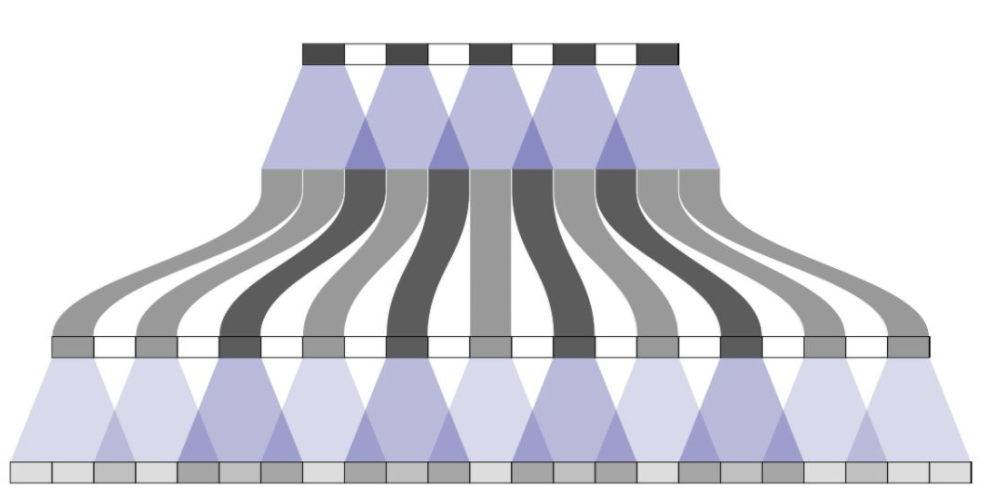
\includegraphics[width=0.5\textwidth]{grid_effect.png}
    \caption{反卷积参数配置不当带来的棋盘效应\citing{46191}}
    \label{grid_effect}
\end{figure}

像素随机化(Pixel Shuffel)的上采样方法现今主要被用于超分辨率工作中,有时也会用于其他计算机任务中。像素随机化的具体思想是输入一个低分辨率的特征,尺寸为表示为$H \times W \times C$, 我们先通过卷积运算对维度进行扩张,得到一个$H \times W \times r^2C$的特征图,最后通过pixelshuffel的操作得到$rH \times rW \times C$,实现上采样的效果。这样的像素随机化的过程可以理解为将这得到的$r^2$的通道的特征图进行打乱重组,得到满足要求的、尺寸扩大的特征图。具体的如图\ref{pixel_shuffle}所示。

\begin{figure}[h]
    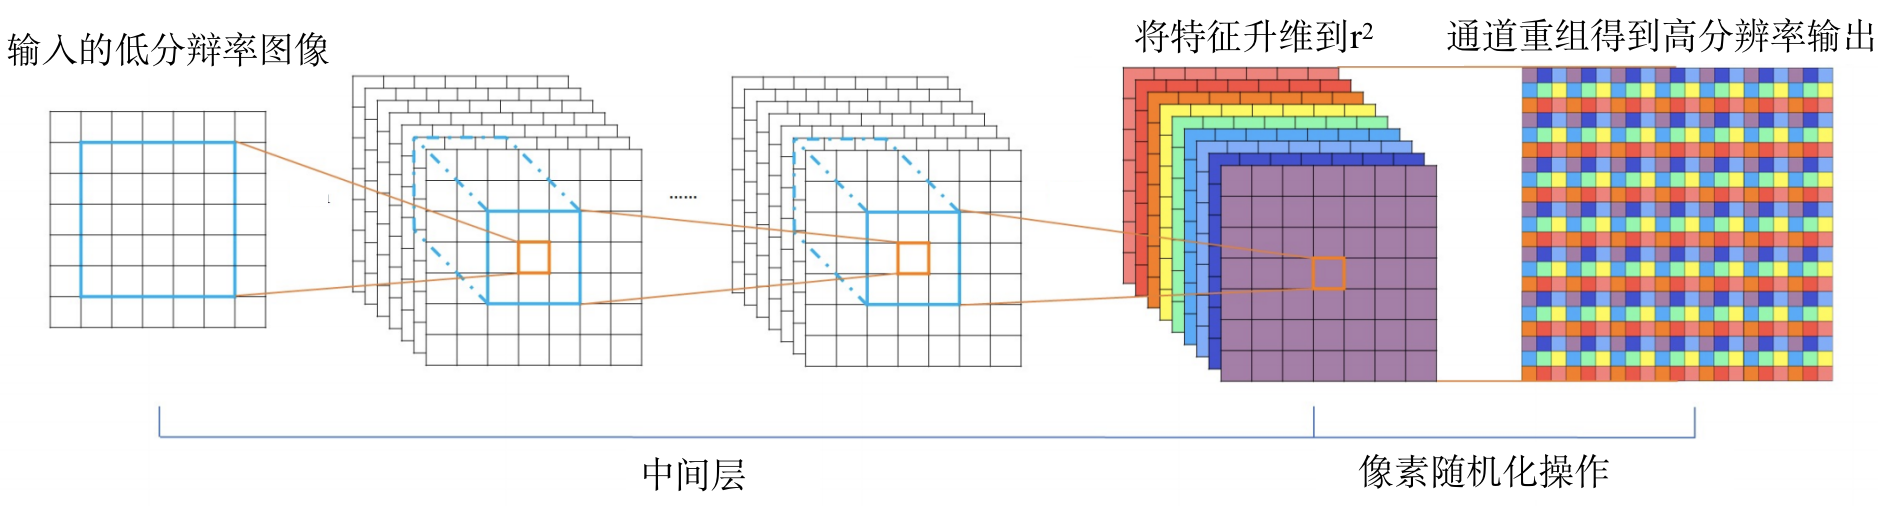
\includegraphics[width=0.95\textwidth]{pixel_shuffle.png}
    \caption{像素随机化上采样方法\citing{PixelShuffle}}
    \label{pixel_shuffle}
\end{figure}

\subsection{膨胀卷积}
在图像像素级理解任务中,为了获取更好的上下文语义信息用于算法对输入图片的全局场景进行判断,从而得到更好的预测结果,我们需要让我们算法的高层特征拥有较大的感受野。而我们在之前提到,随着基于图片识别的主干网络中不断的池化层,高层特征能够拥有较大的感受野,但是随之而来的就是特征分辨率的降低。较低的特征分辨率对稠密预测问题来说也是一个重要的影响因素。总的来收,稠密级的图像理解任务,我们即需要较大的感受野让网络更好的理解输入图像,也需要一个较大的特征分辨率对逐像素进行预测。膨胀卷积的提出能够帮我们达到这样一个目的。

膨胀卷积(dilated convolution)可以理解为采样率大于1的卷积方法,对比\ref{conv_equation}中的卷积方法,膨胀卷积的表达式为,其中$r$为采样率,代表我们在卷积时每多少个像素进行一次采样。如果$r == 1$则退化为普通卷积,可以把普通卷积看成膨胀卷积的特殊形式。通过调整参数$r$,我们可以达到不同的效果:
\begin{equation}
	y[i] = \sum\nolimits_{k = 1}^{K} x[i + r \cdot k] w[k]
\end{equation}

膨胀卷积(如图\ref{dilated_conv})已经广泛应用在了语义分割等稠密级图像理解任务中,并且取得了很好的效果。通过膨胀卷积,能够使图像理解模型获取更大感受野的特征,并且保证分辨率在一定水平上。

\begin{figure}[h]
    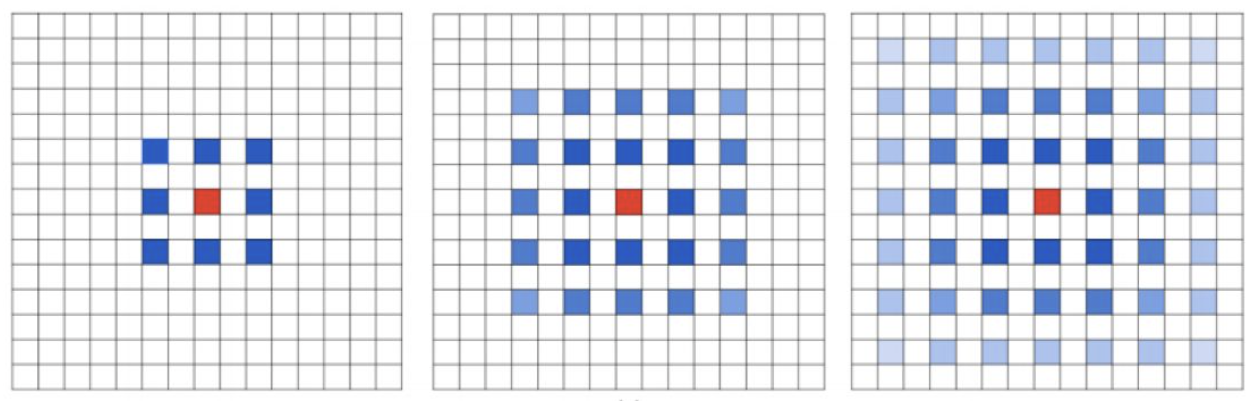
\includegraphics[width=0.55\textwidth]{dilated_conv.png}
    \caption{膨胀卷积的具体采样图示,图中展示了连续3个膨胀卷积的采样结果\citing{DBLP:journals/corr/WangCYLHHC17}}
    \label{dilated_conv}
\end{figure}

从图\ref{dilated_conv}我们同样可以发现,在这种设置下膨胀卷积采样的像素点并不连续,在采样像素中间会有很多像素点被丢失,会损失信息的连续性。然而对于稠密的、像素级的预测任务来说,这种像素连续性上的损失是致命的,会导致很严重的后果。所以我们在设计网络时需要精心设计好膨胀卷积的参数。在之前图森公司的一篇叫做HDC的工作中,有研究者探究了膨胀卷积的设置方法,证明了按照一定规律设置好膨胀卷积的参数能够避免这种情况的发生,充分发挥膨胀卷积的作用。 
\subsection{注意力机制}
注意力机制最早出现在了自然语言处理领域,自从被引入深度学习之后,便在自然语言处理\citing{vaswani2017attention}、计算机视觉\citing{Edge_Attention}\citing{Saliency_Pyramid_Attention}\citing{nonlocal}等各个领域都取得了十分良好的效果。注意力机制的出发点其实非常直接,人类在观察一张图片或者阅读一段文字时,对图片内部或者语句内部,人们的注意力的分布不是均匀的,而且会随着视线的变化进行动态的调整。比如人类在观察一张图片时,我们常常是对图片中某个物体有着很强的关注度,这个物体可能是最近出现过、让人们印象深刻,或者是在图片中占据显著位置。而注意力机制引入神经网络就是借鉴了人脑对信息的处理,通过注意力机制,网络可以动态地学习关注到一些关键的信息进行处理,去除一些冗余的干扰信息,提升算法的处理效率。自然语言处理中经典的网络结构Transformer\citing{vaswani2017attention}便是通过注意力机制达到了良好的效果。

在计算机视觉领域,注意力机制按数据来源可以分为自注意力(self-attention)机制和常规的软注意力机制(soft attention)。按照注意力关注的定位来说又可以分为空间域的注意力(spatial-wise attention)、通道域的注意力机制(channel-wise attention)。

引入自注意力机制的第一篇工作探索是\citing{vaswani2017attention},作者在文中为了对输入的长文本进行有效的理解,引入了自注意力机制让网络能够对输入的文本序列建立长距离的内容依赖关系,促使网络自动地关注长文本中的关键部分。同时在获取全局信息的内容上,全连接层也能达到对整体信息,远距离依赖建模的能力,但是全连接层无法处理任意长度的输入序列。而自注意力机制能够动态地对变长序列生成不同的权重,对任意长度序列进行处理。

在2018年的工作Non-local\citing{nonlocal}中,自注意力机制第一次被引入到计算机视觉领域,卷积神经网络中的卷积层只关注一个小的领域内的目标,随着卷积层的不断堆叠,感受野的逐渐扩大,对于长序列的视频文件也难以达到全局依赖的获取能力。有研究工作证明了网络在高层的实际感受野会远远小于计算出的理论感受野大小。所以作者引入了自注意力机制用来长距离依赖。对于输入的视频来说,获取长序列视频全部帧中的每个像素,和当前像素的一个相似度关系,这个关系能够对长时间依赖进行建模,引入全局的信息(图\ref{non_local})。具体的公式化表达如下,其中$f(x_i, x_j)$代表两点之间的相似度,有很多种计算方法,$g$用于做一次特征变换,$N$为归一化因子。

\begin{equation}
    \label{self_attention}
    y_i = \frac{1}{N} \sum_{\forall j} f(x_i, x_j)  g(x_j)
\end{equation}


\begin{figure}[h]
    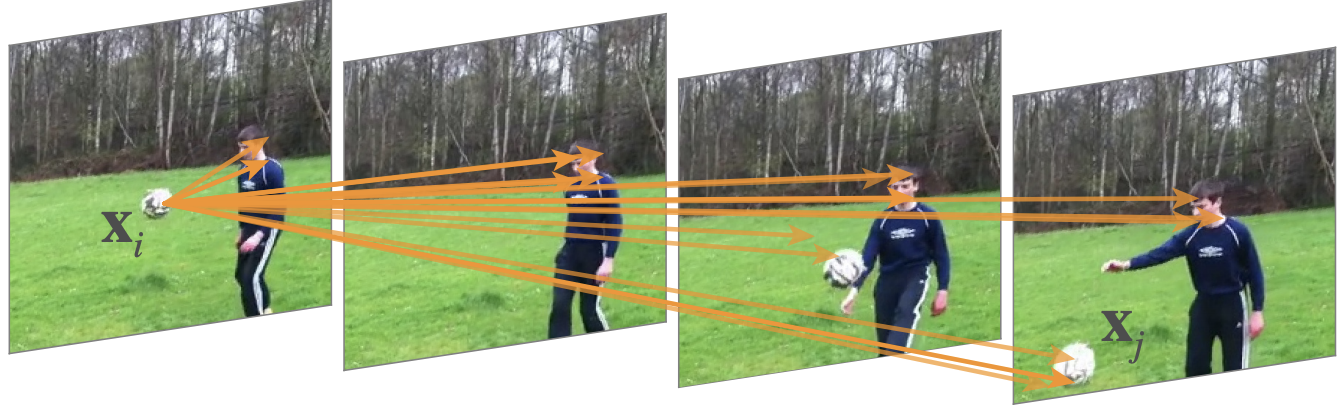
\includegraphics[width=0.65\textwidth]{non_local.png}
    \caption{自注意力机制对视频相似度的建模\citing{nonlocal}}
    \label{non_local}
\end{figure}

此外自注意力机制还可以用于2D图像上的长距离依赖的建立,通过2D图像的自注意力机制,我们可以获取当前图像的所有其他像素点和当前像素点之间的相似度$f(x_i, x_j)$,从而引入全局信息帮助网络对图像进行处理。这样的自注意力机制已经被广泛应用于图像理解中的语义分割任务(引用)中,并且取得了良好的效果。值得注意的是,因为需要计算每个像素和其他所有像素之间的相似度,所以自注意力机制的计算复杂度和 显存占用很大,所以常见的分割中的自注意力机制都是在最后一层小特征图上进行的。除此之外,也有很多研究者\citing{CCNet}\citing{A2Net}\citing{yue2018compact}\citing{PSANet}\citing{OCNet}利用先验知识和近似算法降低自注意力机制的复杂度,也取得了不错的效果。在语义分割中,我们可以将自注意力机制理解为学习像素点到语义点的映射,并且根据对应语义点,再反映射回对应的像素,根据全局信息赋予像素更准确的语义信息。在自注意力机制中,也可以结合通道域和空间域上的自注意力机制达到更好的效果,相关的研究已经在语义分割中得到了良好的效果。\citing{DANet}对于后续图像上的自注意力机制,像素之间相似度的计算方法通常如下所示,其中$\theta$和$\phi$代表特征转换,在实际应用中常常是一层卷积层达到对应特征转化效果,转化过后的结果常常被称为query和key。得到对应的相似度关系的情况下,再根据公式\eqref{self_attention}可以得到自注意力机制最后的结果。2D图片上空间域的整个流程可以描述为:先利用三个不同卷积层$\theta$、$\phi$和$g$对输入的特征进行特征变换,得到query、key和value。之后利用query和key的内积计算得到对应的相似度矩阵$f(x_i, x_j)$,在将相似度矩阵作用在value上,得到最后的结果。在通道域上的流程和上述类似,区别在于计算不同特征通道之间的相似度。
\begin{equation}
    f(x_i, x_j) = \theta(x_i)^T \phi (x_j)
\end{equation}

软注意力机制(soft attention)常常被用作门(gated)机制,已经广泛应用在了图片分类\citing{SENet}、图片分割\citing{takikawa2019gated}、目标检测\citing{zeng2016gated}、显著性检测\citing{zhang2018bi}等各个计算机视觉领域中。门机制的作用可以简要概述为:网络可以利用相关特征来学习一个注意力的分布,并且用这个动态学习的注意力的权重图作用在特征上,来对特征进行进一步的提取和加强,提取其中的关键信息,削弱一些冗余的部分。 软注意力机制可以被用在不同的作用域中,包括用于空间域上对空间上的信息进行进一步提取加强、用在通道域上对不同通道的特征重新计算权重、还可以利用其他时刻或者其他层次的特征作为注意力机制的权重图指导当前特征关键信息的提取\citing{kosiorek2017hierarchical}\citing{wang2017residual}\citing{SENet}。我们定义输入的特征为$x$, 输出特征为$O$,若要根据特征$x$对其进行空间或者通道上的注意力机制,则按下式进行: 其中$A$代表sigmoid激活函数,$P$代表全局池化层,$\theta$代表卷积层。
\begin{equation}
    \label{spatial_attention}
    O = A(\theta(x)) *  x 
\end{equation}
\begin{equation}
    \label{channel_attention}
    O = A(P(\theta(x))) *  x 
\end{equation}

通过上述注意力机制,我们能够对于任意尺寸的输入的图片,自动化地获取其全局信息和语义信息,并且使得网络能够动态地选择特征中空间或者通道上的关键信息,达到良好的效果。

\section{边缘检测算法}
在上面一节中,我们介绍了在实现中会接触到的深度学习的基础知识,包括基本的卷积神经网络的各部分组件、图像理解常用的上采样模块和膨胀卷积模块,并且简单介绍了几种注意力和它们的效果。在这一章中我们将介绍边缘检测任务,并且介绍传统领域和深度学习领域的经典方法。从这些经典方法中,我们能够知道我们研究的一个基线和一个出发点,有助于更好的理解我们的工作。

\subsection{边缘检测任务}
图像理解任务是机器学习的一大重要任务,而边缘检测任务又是图像理解任务的一个基本步骤和关键基础。本小节我们给出图像边缘检测的定义,给定一个二维的图片$I$,分辨率为$H \times W \times 3$, 我们需要对给定图片$I$中的每一给像素点$p$,判断它是否是边缘点,是一个稠密预测的二分类问题。输入图片的分辨率越大,对于单张图片来说边缘检测需要的计算量越高。边缘检测任务不仅可以作为后续分割、检测任务的基础任务为上游任务提供数据,也可以作为分割、检测的一部分提高上游任务的预测效率。图\ref{edge_detection}是一个边缘检测任务的基本输入和输出图示。

\begin{figure}[htb]
    \centering
    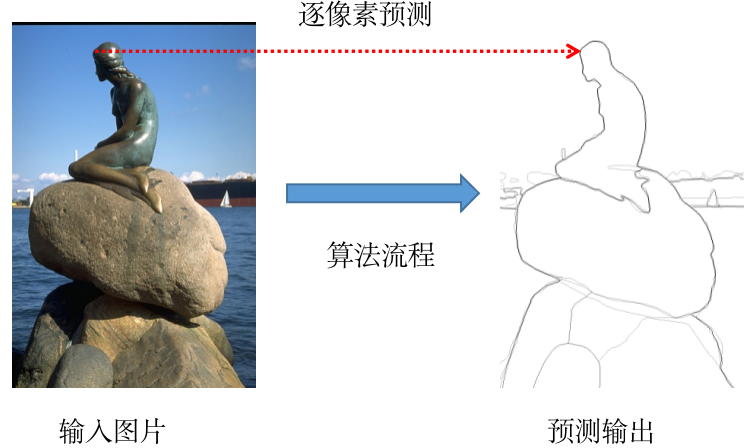
\includegraphics[width=0.5\textwidth]{edge_detection.png}
    \caption{图像边缘检测任务基本图示}
    \label{edge_detection}
\end{figure}

\subsection{边缘检测任务经典方法}

边缘检测任务的研究可以追溯到上世纪六七十年代,作为计算机视觉领域的基石性任务,在很早就获得了人们的关注。现在的边缘检测方法可以分成两大类:基于传统计算机视觉的边缘检测算法(hand-crafted)和基于深度学习的边缘检测算法(deep learning)。 其中深度学习的边缘检测算法又可以分为:利用深度学习提特征的多阶段检测算法和端对端的边缘检测算法。最近几年人们对于边缘检测算法的研究主要在 端对端的算法上,因为端对端的算法能够取得更高的精度和速度,同时因为不需要多阶段处理,具有很强的实用性。在最近人们对端对端边缘检测算法 的研究中,又可以分为三个结构:HED结构、自顶向下结构和自底向上的结构。图\ref{edge_detection_xmind}是具体的边缘检测算法的分类图。
\begin{figure}[h!]
    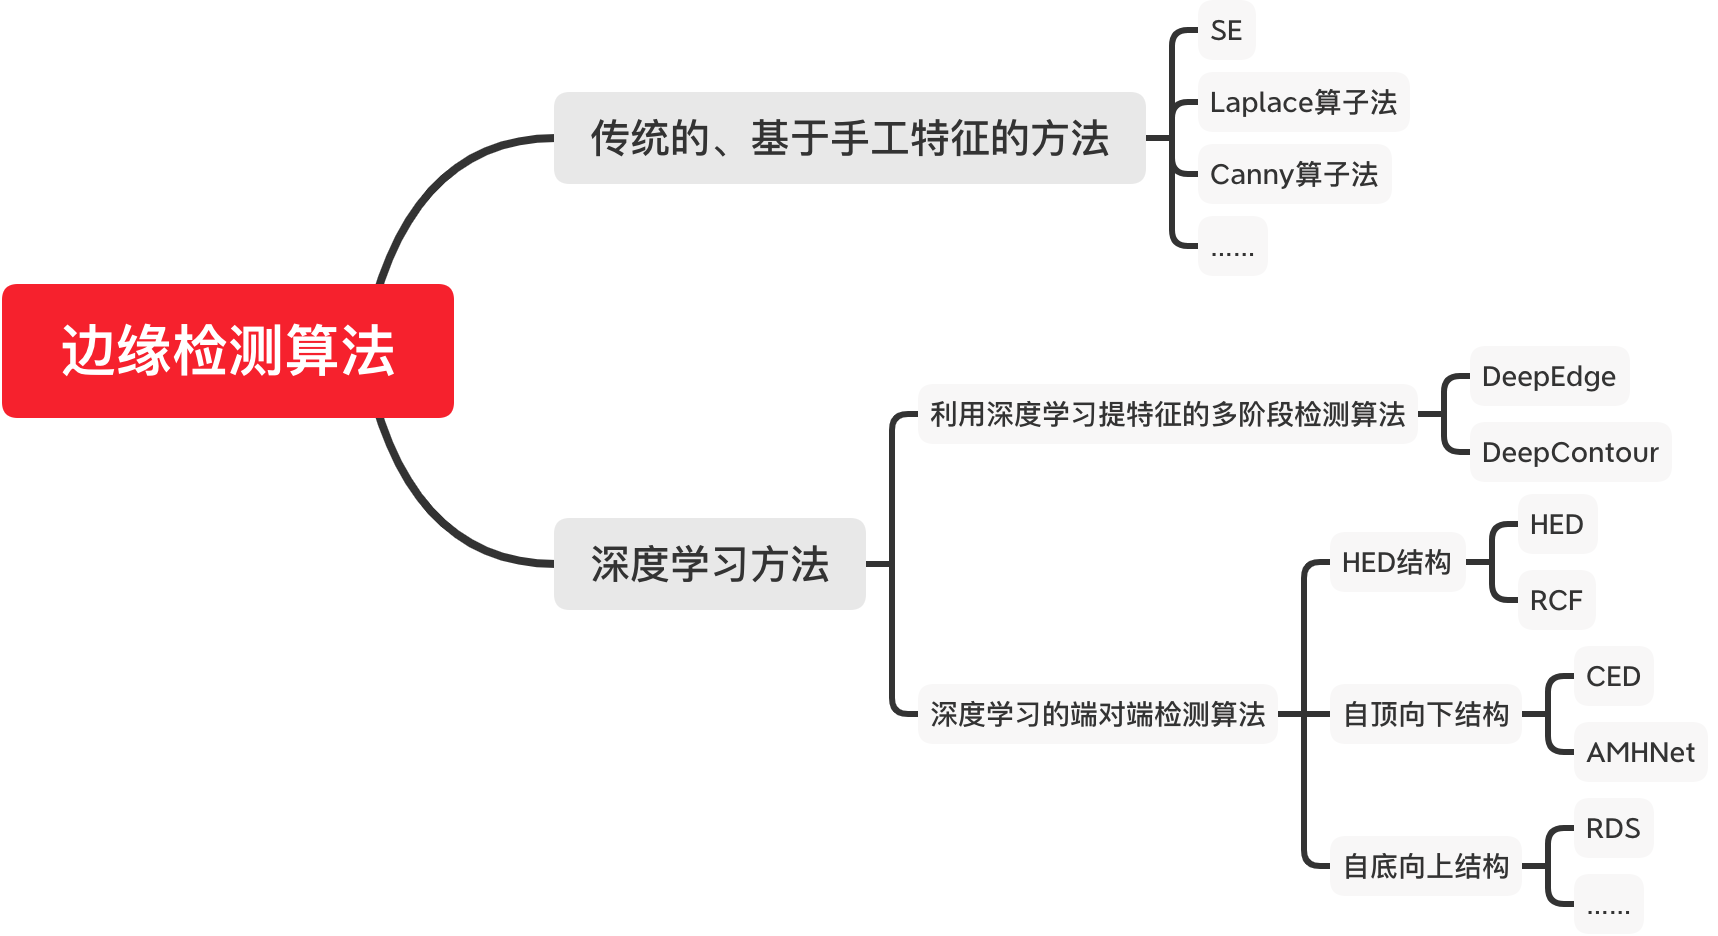
\includegraphics[width=0.95\textwidth]{edge_detection_xmind.png}
    \caption{图像边缘检测方法的分类描述}
    \label{edge_detection_xmind}
\end{figure}
我们将介绍一个最著名的传统方法Canny算法\citing{Canny}和最经典的端到端深度学习方法HED\citing{HED},对它们的介绍将有利于读者在后续充分理解我们提出方法的创新和贡献。

Canny算子法是最有名的传统边缘检测算法,已经被集成进了Matlab的工具箱中,使用者可以通过一行命令简单的调用就能实现该算法。该算法是基于图像局部灰度变化的剧烈情况来对边缘进行检测和识别的,同样也存在一般传统算法缺失全局语义信息的问题,但是因为它流程简单、计算快速,在很多情况下也被选为使用的边缘检测算法。

Canny算子法主要分为五个步骤:

1)利用高斯滤波器对输入图像进行降噪。在传统的图像处理方法中,因为输入图像可能带有各种各样不同的噪声,影响图像处理最后的结果。所以在传统图像处理之前,通常都会进行降噪处理。在Canny算子的方法中,我们利用高斯滤波器的对图像进行降噪处理。高斯滤波器可以过滤掉图像上的高斯噪声。高斯核函数的表达式如下所示:
\begin{equation}
    \label{gaussian}
    G(x, y) = \frac{1}{2  \pi \sigma ^ 2}e^{- \frac{x^2 + y^2}{2\sigma^2}}
\end{equation}

\begin{equation}
    O(x, y) = G(x, y)* I(x, y)
\end{equation}
其中$x$和$y$分别表示图像上的一个像素点的坐标在分别代表高斯滤波的过程中,高斯滤波器在核的一个小邻域内可以类比为一个金字塔结构。对于目标像素点$p$,来说在一个滤波器中离点$p$距离越远的权重越小,可以理解为用如上\ref{gaussian}所示的高斯核对整个图像在一个小的领域内执行加权求和平均的计算。特别的,对于图片上每个像素点,都是由像素点本身和周围一个小的领域内的点加权平均得到。通过高斯滤波,可以去除图片的噪声,使得图片在视觉效果上变得模糊。同时因为模糊的因素,也可能增加图片中边缘的宽度。

2)在降噪处理之后的图片上计算像素的梯度值和梯度方向。 梯度的概念在数学中表现为函数的微分,例如在微积分中对二维函数的一阶微分可以表示为:
\begin{equation}
    \frac{\partial f(x, y)}{\partial x} = \lim_{\epsilon \to  0} \frac{f(x + \epsilon, y) - f(x, y)}{\epsilon }
\end{equation}
\begin{equation}
    \frac{\partial f(x, y)}{\partial y} = \lim_{\epsilon \to  0} \frac{f(x, y+ \epsilon) - f(x, y)}{\epsilon }
\end{equation}
通过在数学上的定义,我们可以引申到图像领域来,图像领域的梯度代表了当前像素点$p$在x轴方向和y轴方向的灰度变换的快慢。而因为像素在图片上表现出的离散的特性,在计算图像梯度时,我们不需要进行微积分的极限运算,而只需要进行简单的加减运算,利用差分算子计算得到图像梯度。通过上一步高斯滤波器的降噪处理,我们已经排除了图片上几乎大部分噪声。在人们传统的定义中,将边缘定义为两个区域的区域边界、分割线,那么在分割线区域就会出现剧烈变化的灰度值。我们可以对整张图片的每隔一个像素计算其灰度值变化的剧烈情况,求可以得到对应的边缘点。在Canny算法中常用的算子是Sobel算子,它的形式如下式所示:
\begin{equation}
    G_x = 
        \left[
        \begin{matrix}
          -1 & 0 & 1 \\
          -2 & 0 & 2 \\
          -1 & 0 & 1
         \end{matrix}
        \right] 
    , G_y = 
    \left[
        \begin{matrix}
          1 & 2 & 1 \\
          0 & 0 & 0 \\
          -1 & -2 & -1
         \end{matrix}
        \right] 
\end{equation}
可以很明显的发现Sobel就是计算一个像素为中心的领域内在x轴方向和y轴方向上的差分。通过Sobel算子点乘输入的图片$I$,我们能够计算得到图片中每个像素点$(p, q)$上的在x轴方向上的梯度$g_x(p, q)$和y轴方向上的梯度$g_y(p, q)$。  我们进而通过公式\eqref{gradient_value}得到该点处的梯度大小, 通过公式\eqref{gradient_direction}得到对应的图像梯度方向:
\begin{equation}
    \label{gradient_value}
    G(p, q) = \sqrt{g_x(p, q)^2 + g_y(p, q) ^ 2}
\end{equation}
\begin{equation}
    \label{gradient_direction}
    \theta = arctan \frac{g_y(p, q)}{g_x(p, q)}
\end{equation}

3)使用非极大值抑制(Non-maximum Suppression)过滤不是边缘的点,将边缘变细。进过上一步计算的得到的梯度图像存在着边缘粗而宽,并且存在大量弱边缘的问题,我们需要利用非极大值抑制的方法去寻找像素在一个领域内的局部最大值,然后将非极大值对应的灰度设置为0,从而去除弱边缘和边缘附近的模糊情况。在实现边缘非极大值抑制的实现中,对图输入梯度图片上的每一个点$G(p, q)$,我们在以$(p, q)$为中心的一个$3 \times 3$临域内判断局部极大值,这里的$3 \times 3$邻域可以堪称已像素点$p$为中心的8邻域内。对于点$G(p, q)$,我们记为点$p$,我们可以通过在点$p$的梯度角信息$\theta_p$确定这个点边缘法线的朝向。我们可以将朝向分为4个模式,即x、y和两个对角方向。根据梯度角$\theta_p$的值判断法线在哪个朝向模式内部。如图\ref{nms}所示该点的梯度角$\theta_p$的模式在x轴方向,所以点$p$需要和点$q$、点$r$相互比较。若点$p$的值大于点$r$和点$q$的值,则点$p$的值为局部极大值,进行保留。否则说明另外某点对边缘的响应程度要大于点$p$对边缘点的响应程度,则点$p$不在真正的边缘点上,需要抑制点$p$。
\begin{figure}[h!]
    \centering
    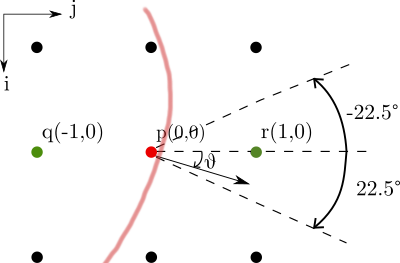
\includegraphics[width=0.4\textwidth]{nms.png}
    \caption{边缘检测中非极大值抑制的运行机制}
    \label{nms}
\end{figure}
需要说明的是,在后续深度学习方法得到的边缘预测结果同样需要非极大值抑制处理才能得到最后的结果,在现今的方法中,这已经成为边缘检测任务中的必备模块。

4)利用两个阈值进一步判断边缘,对结果进行二值化。利用两个阈值max和min分别 对边缘进行二值化操作。二值化规则:对应结果大于阈值max的被认为是边缘,低于阈值min的被认为是非边缘点。而对于值在max和min之间的像素点来说,其是否是边缘点根据和已经被判断为边缘点的邻接关系判断。如果和边缘点邻接,则判断为边缘,否则不是。 我们可以从已被判断为边缘的点开始扩张 ,进而进行判定。在递归对中间值的点进行判定的情况下,利用 递归判断的计算代价很大,在弱边缘点数很少的情况,可以在一定情况下放弃该步骤换取更快的计算速度,值得注意的是,这里的阈值max和min,需要人们手工选取,这个阈值的选取对最后得到的展示结果也有很大影响。


在深度学习时代,最开始应用于边缘检测领域的方法是DeepEdge\citing{DeepEdge}和DeepContour\citing{DeepContour},它们仅仅利用深度学习来提取高阶特征用于替代传统方法的手工特征用于边缘检测,但是需要多阶段的处理才能得到预测的边缘检测结果。2015年的HED\citing{HED}是第一个实现端对端推理预测的深度学习边缘检测方法,奠定了深度学习时代边缘检测的基本架构,我们将详细介绍这片文章的工作。而这篇文章的基本结构也将作为我们论文后续对比的基线方法(Baseline)。

HED全称是Holistically-Nested Edge Detection,是发表在2015年ICCV上的会议文章,可以通过深度学习自动学习特征并且自动进行预测。在HED算法中,采用了VGGNet这一个图片识别网络结构在作为算法的主干网络,用于提取输入图像的特征。VGGNet有16层卷积层和全连接层构成,原始的网络中全连接层被使用做分类器对输出进行分类,而在边缘检测网络中我们仅仅使用VGGNet中的卷积层帮助我们提取特征。VGGNet的卷积层可以分为五个大的模块,从浅层到高层我们可以将其称为stage$1,...,5$。利用VGGNet,我们可以从输入图片提取到从底层到高层总共5个层次和尺度的特征,这样多尺度的特征也为最后的结果提供了极大的帮助。网络的推理流程可以总结如下:输入一张2D图片$I \in H \times W \times 3$, 利用VGGNet提取其特征得到$f_1, f_2, ..., f_5$,其中$f_1 \in H \times W \times 64, f_2 \in \frac{H}{2} \times \frac{W}{2} \times 64,  f_3 \in \frac{H}{4} \times \frac{W}{4} \times 256,...$。在得到对应的五层特征之后,网络分别让它们通过连续的$1 \times 1$卷积进行降维操作在通道降维为1。之后通过一个双线性插值(bilinear interpolation)对特征进行上采样,将五层特征的宽高全部统一成输入尺寸$H \times W \times 1$。此时我们得到了五个侧枝的成输出,我们记为side-output1, side-output2,..., side-output5。为了得到最后的输出我们将所有侧枝输出拼接在一起得到$H \times W \times 5$的特征,并且通过$1 \times 1$的卷积降维为$H \times W \times 1$的最终输出。图\ref{hed}是网络的整体结构图。图中可视化了网络得到了5个不同层次、在不同感受野条件下的边缘表达。
\begin{figure}[h!]
    \centering
    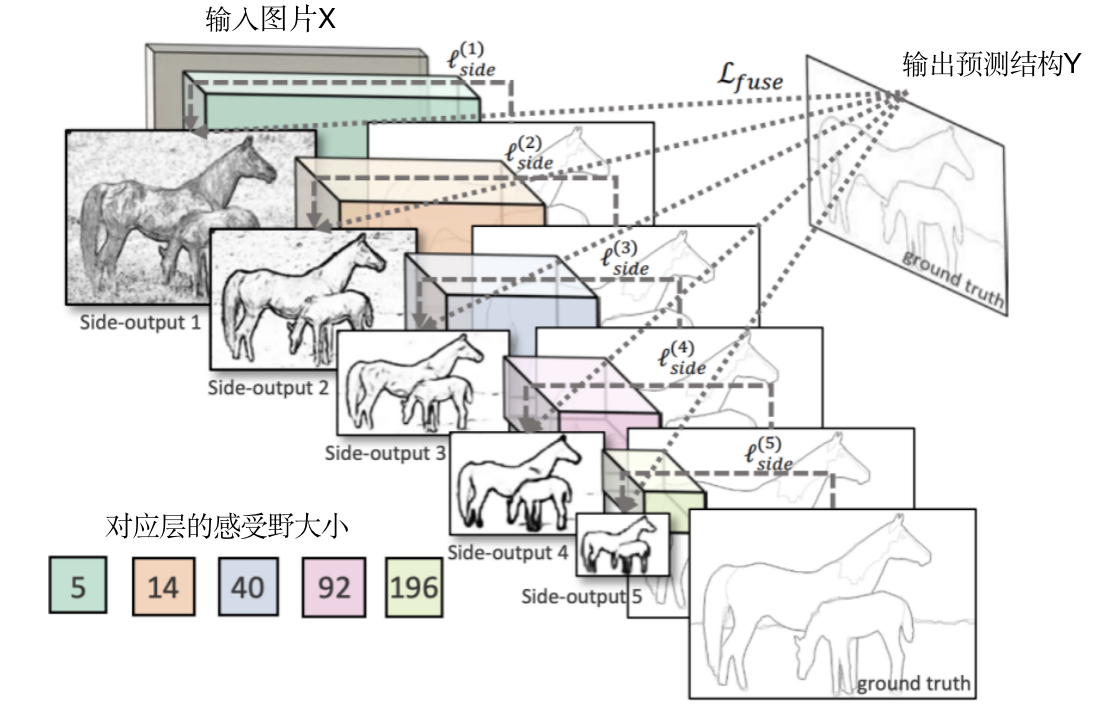
\includegraphics[width=0.5\textwidth]{hed.png}
    \caption{HED网络结构图\citing{HED}}
    \label{hed}
\end{figure}
HED网络在当时取得了良好的精度和速度,并且证明了神经网络提取的高层语义特征对于边缘检测的作用,从特征的可视化中我们可以发现,高层特征得到的边缘表达中不会收到细小噪声的印象,并且能够获取大物体的整体轮廓。对于底层局部特征预测出的边缘具有修正作用,这一个观察也是边缘检测算法的一个重大出发点,它证明了对于边缘检测的多尺度特征合成的必要性,这也证明了本文研究的重要性和必要性。

在HED中使用的损失函数是带权重的二分类交叉熵函数,并且作者对所有层次输出的边缘特征和最终边缘特征都使用了对应的真值进行监督。对于输入的图片$I$,对于每个侧枝输出,带权重二分类交叉熵函数表示如下:
\begin{equation}
l_{side}^{(m)} = - \beta \sum_{j \in Y_+} logPr(y_j = 1 | I; W, w^{(m)}) - (1 - \beta)  \sum_{y \in Y_-} logPr(y_j = 0 | I; W, w^{(m)})
\end{equation}
其中m代表对应所在的层次,$W$代表网络了网络的整体参数,$w^{(m)}$达标了对应不同侧枝输出在线性加权为最终结果时的权重,即网络如果有M个侧枝输出的化,那么定义$w = (w ^{(1)}, w ^{(2)}, ..., w ^{(5)})$。其中$\beta$为平衡正负样本的权重系数。我们在对边缘检测进行定义时候,就能发现这个问题的一些需要注意的点:正负样本极度不平衡。为了加强正样本权重,这里使用了$\beta$参数。$\beta$定义为$\frac{|Y_-|}{|Y|}$,其中$|Y_-|$代表输入图片中所有非边缘点集合,而$|Y|$代表了输入图片的全部像素点。 因为非边缘点个数$|Y_-|$总是远远大于$|Y_+|$, 所以正样本也动态地拥有了更大的权重系数。$Pr(y_j = 1 | I; W, w^{(m)})$代表了测试网络输出的边缘表达结果,其中$Pr()$是Sigmoid激活函数。

最终所有损失函数的表达式为:
\begin{equation}
L(W, w) = \sum_{m = 1}^{M} \alpha_m l_{side}^{(m)}(W, w^{(m)})
\end{equation}
其中$\alpha_m$代表损失函数的权重系数,用于平衡不同侧枝网络的损失函数。图\ref{hed_visual}展示了网络的输出结构和真值的对比。除此之外,还展示不同的侧枝网络输出对应的结果,图中展示了side-output2, side-output3, side-output4的结构,可以发现随着 特征的层次逐渐提高,网络中的噪点越来越少。高层次的特征能够更好的反应物体整体的轮廓,但是高层次的同时伴随着细节边缘的减少和分辨率的降低。这个展示也进一步引出了我们后文的主要研究点和研究目的。
\begin{figure}[h!]
    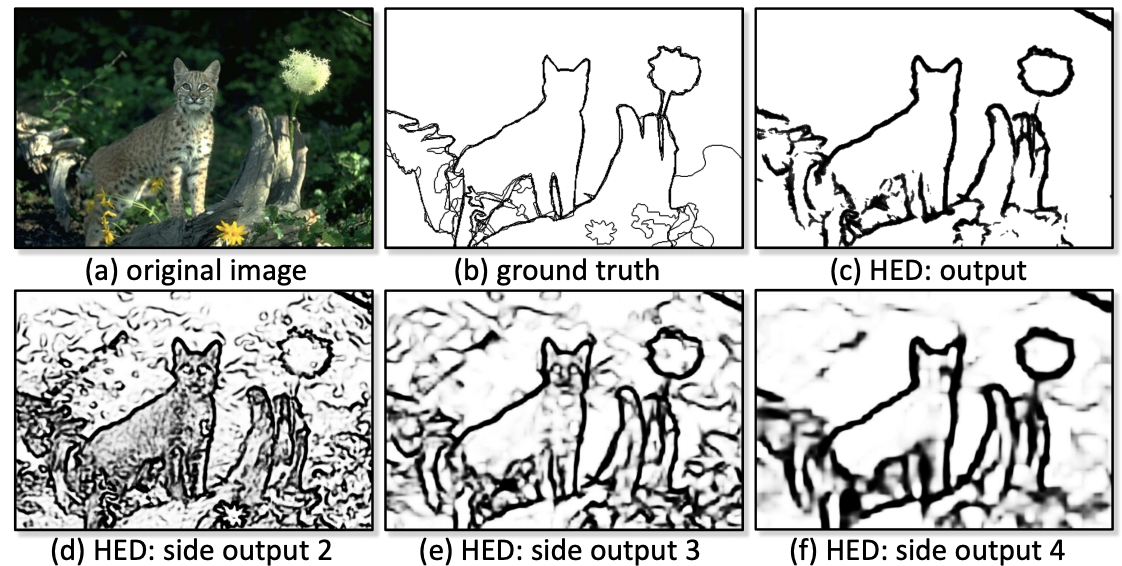
\includegraphics[width=0.8\textwidth]{hed_visual.png}
    \caption{HED网络的中间层结果输出可视化\citing{HED}}
    \label{hed_visual}
\end{figure}
在HED提出之后,后续有很多相关改进工作。例如RDS提出对HED不同的侧枝网络生成的对应的不同的真值对每个侧枝网络进行监督,RCF\citing{RCF}通过对提取VGGNet的每一层卷积的特征,从而达到提取更丰富的特征的作用,都取得了不错的效果。

% \begin{algorithm}[H]
%     \KwData{this text}
%     \KwResult{how to write algorithm with \LaTeX2e}
%     initialization\;
%     \While{not at end of this document}{
%         read current\;
%         \eIf{understand}{
%             go to next section\;
%             current section becomes this one\;
%         }{
%             go back to the beginning of current section\;
%         }
%     }
%     \caption{How to wirte an algorithm.}
% \end{algorithm}


\section{本章小结}
在本章节中,主要介绍了卷积神经网络的重要组成部分,包括卷积层、池化层、激活函数层、全连接层这几个部分。介绍了图像理解中的重要概念包括感受野、上采样等。同时我们还介绍了注意力机制的概念和它的基本现状,这一机制也是我们会在自己的工作中有所使用的。除此之外,我们还介绍了边缘检测任务的基本定义、发展脉络的分类,通过对传统领域经典方法Canny算子法和深度学习领域基石性方法HED的介绍,能够对边缘检测有一个清晰的认知,有利于理解我们本文作出的贡献。

\chapter{基于自底向上的渐进网络优化边缘检测算法}
随着深度学习的逐渐发展,在边缘检测领域已经出现了越来越多的基于深度学习的方法,并且取得了良好的效果。研究者们基于HED网络的改进取得了明显的效果,这些方法也推动了边缘检测领域这几年的进步。过去的方法已经证明了提取不同尺度的特征用于最终的预测能够达到更好的预测效果。但是利用深度学习来实现边缘检测仍然有一些没有解决的问题。从上文的描述中,我们可以发现深度学习边缘特征表达,对不同尺寸特征下的边缘有不同的表现结果。从卷积神经网络浅层提取出的浅层边缘特征能够编码一些低层次的空间信息例如边缘,角点等,但是会伴随着大量的噪点;而卷积神经网络深层提取到的高层次边缘特征能够编码物体级别(object-level)的信息,这些信息包含物体的大体轮廓,同时对于局部特征产生的噪声有着很好的抑制作用,这些不同层次的特征表达是互补的,并且对于提高最终边缘检测的效果有着很好的帮助作用。 

得益于卷积神经网络对于图像特征的多层次提取,这也促使我们设计更好的网络用于结合多层次特征从而达到更好的网络效果。 对于经典的HED网络来说,所有的侧枝输出都是独立进行处理的,最终的结果是通过将侧枝网络的所有输出做线性加权得到最后的结果。然后对于简单的线性加权并不能挖掘神经网络多层次特征的关系,将最终结果限制在一个线性空间中,只能达到一个次优的结果。为了挖掘一个更好的结合方式,我们提出了基于自底向上的渐进网络优化边缘检测算法。同时考虑到边缘检测任务中通常面临着公开数据集规模过小,缺乏训练数据,然而测试集上的物体有着不同比例的大小关系。鉴于普通的网络很难从小数据集上学习感知多尺度的物体。我们应该了大量的图像增强技术,并且引入膨胀卷积和特征金字塔池化层。特征金字塔池化层用于提高网络对自然环境中各类比例、大小物体的感知能力。而通过膨胀卷积,我们能够实现在保证特征图分辨率大小不变的情况下,提高对应特征图感受野的效果。

对于上述提到的多特征融合问题,考虑到高层特征和低层特征具有的特征,我们可以考虑到利用带有物体轮廓信息和丰富语义信息的高层特征为结合提供额外的信息。我们可以将高层特征作为指导信息,帮助低层特征去除若边缘点和错误预测的噪点。渐进的让侧枝网络基于对应的高层特征指导,去除低层特征的额外信息仍然是一个有挑战的任务。基于此,我们在侧枝网络中引入了注意力机制,让网络自动学习并且动态地关注到需要去除噪点和若边缘的区域。这样一个注意力机制的引入能够让整个侧枝网络的引导合成效果变得更好更鲁棒。低层特征在渐进优化的过程中可以保留其丰富的细节信息,并且丢弃对应的噪点和若边缘点,最终达到一个较好的结合结果。

通过上面的观察和思考,概括来说,在这个工作中的主要贡献为:

1)我们提出了一个基于自底向上的渐进网络优化边缘检测算法。网络能够通过对高层特征和低层特征的渐进式学习,高层特征能够作为指导信息指导低层特征保留它丰富的细节信息,移除不必要的若边缘信息和噪点,从而最终得到准确和高分辨率的边缘检测结果。

2)我们提出了一个渐进性的残差注意力模块用于在侧枝网络中逐层地指导高层语义特征和低层特征的合成,帮助低层特征更鲁棒地移除错误预测的边缘和噪点。

3)同时引入了膨胀卷积和特征金字塔池化层。特征金字塔池化层用于让网络对于不同大小物体有更强的泛化能力。膨胀卷积用于实现维持特征图分辨率并提高对应特征图感受野的效果。

4)我们在两个公开数据集上进行了实验,发现我们提出的基于自底向上的渐进网络优化边缘检测算法能够在BSDS500和NYUDv2上达到了当时业界领先的效果。在BSDS500上 达到了81.9\%的ODS值,83.5\%的OIS值和86.2\%的AP,在NYUDv2上达到了76.2\%的ODS,78.1\%的OIS和79.7\%的AP值, 在两个指标上都领先当时业界的其他方法。


\section{基于自底向上的渐进网络总览}
在本节中,我们将详细介绍提出的基于自底向上的渐进网络边缘检测算法,其中可以主要分为主干网络、特征金字塔网络、基本残差处理单元和注意力模块这几个部分。其中基本残差处理单元和注意力模块共同达成了侧枝网络的渐进优化效果。而主干网络和特征金字塔网络则用于对输入图片特征的提取和加工。整个网络的结构图如图\ref{framework1}所示。

网络的是输入图片定义为$I$,对应的真值图片定义为$G$。通过基于自底向上的渐进网络边缘检测算法,我们能够得到一系列的边缘预测结果$\{E_1, E_2, E_3, E_4, E_5\}$,其中我们将渐进优化的最终边缘输出$E_5$作为网络的最终输出。
\begin{figure}[h!]
    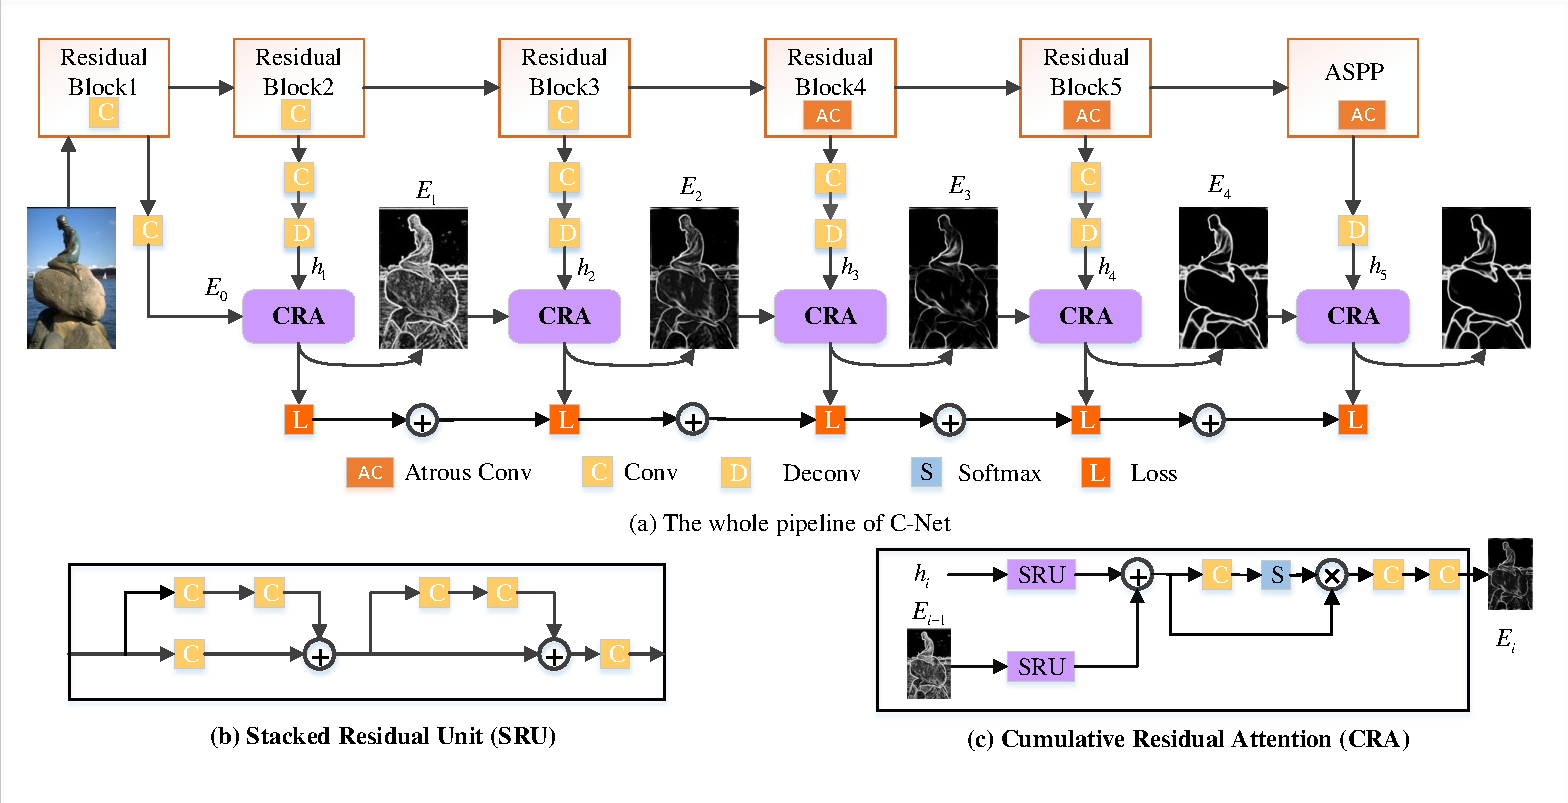
\includegraphics[width=1.0\textwidth]{framework1.pdf}
    \caption{基于自底向上的渐进网络优化边缘检测算法框架图。(a)网络整体结构可以分为3个部分,其中用于提取图片特征主干网络部分、用于对提取特征进行加工增强,提高特征对多尺度物体感知能力的特征池化金字塔模块、对主干网络和特征金字塔网络特征进行处理的渐进优化注意力侧枝网络; (b) 基本残差单元模块,用于在侧枝网络中对特征做进一步提取和分析 ;(c)侧枝网络中的主要模块,用于接受上一层的边缘输入和当前层的特征输入,通过残差单元和注意力机制的作用,输出渐进融合之后的边缘图}
    \label{framework1}
\end{figure}
网络的输入图片为$I \in H \times W \times C$,通过基于图像识别的主干网络提取输入图片的特征,从网络浅层到高层得到的对应的特征$\{f_1, f_2, f_3, f_4,f_5\}$。其中$f_1$对应主干网络第一层的特征,以此类推。可以发现$\{f_1, f_2, f_3, f_4 f_5\}$由于主干网络中不断的池化层操作特征尺寸是逐渐递减的。之后网络将主干网络最后一层的输出特征$f_5$传递为特征池化金字塔模块,经过特征金字塔模块之后得到特征$f_6$。此时特征$f_6$通过特征金字塔模块的处理之后,拥有感知多尺度图像输入的能力。得到了$\{f_1, f_2, f_3, f_4,  f_5, f_6\}$特征之后,我们需要对这些特征进行处理传入侧枝优化网络处理。对于特征$\{f_2, f_3, f_4,  f_5, f_6\}$,我们首先利用卷积对其进行降维,之后利用反卷积模块将对应的特征上采样到输入图片大小$H \times W$,得到一组特征$\{h_1, h_2, h_3, h_4 h_5\}$。对于特征$f_1$,因为其尺寸和输入图片相同,所以不需要经过反卷积上采样模块。在侧枝网络中,对于第一部分的渐进残差注意力模块,它的输入是$f_1$经过卷积处理之后得到的第一层边缘预测结果$E_1$和$f_2$经过卷积和反卷积处理得到特征$h_1$。通过渐进残差注意力模块和对应的输入$E_1$和$h_1$,网络得到了$E_2$,作为渐进网络第二阶段的边缘预测结果。以此类推,通过渐进残差注意力模块,我们能够分别得到剩余的$E_3, E_4, E_5$,其中$E_5$是网络最终的输出。从图\ref{framework1}中我们可以发现,在侧枝网络中预测得到的$E_1, E_2, E_3, E_4, E_5$,从浅层到高层能够逐渐取得更加理想的结果。

\section{特征提取网络和特征金字塔网络}

对于边缘检测任务来说,常常遇到两个问题会影响网络训练,使得网络训练难度增大:缺乏数据集和梯度消失问题。在广泛使用的公开数据集中BSDS500\citing{gPB}和NYUDv2\citing{NYUD}中,BSDS500数据集中总共只有300张训练图片,而NYUDv2数据集总只有765张训练图片。从一个随机初始化中训练一个边缘检测网络是一个很困难的事情,所以我们利用已经训练完毕的图像识别网络作为主干网络,将之前在图像识别任务上训练好的参数作为主干网络参数的初始化。考虑到梯度消失问题,我们试图引入跳层连接,由此我们选取了在图像识别网络取得良好效果的残差网络(ResNet)\citing{ResNet}。残差网络中存在的大量的跳层连接,为梯度回传提供了极大的便利,同时已经在图像识别领域取得了良好的效果。

因为边缘检测检测任务和图像识别的区别,图像识别对于输入图片输出一个特征向量用于分类,而边缘检测需要对输入图片每一个像素对于输入图片的每一个像素都做一个分类,对特征分辨率的要求更高;我们更进一步期待网络能够输入任意大小的图片而不是在图像识别中固定为某一个尺寸,这样有利于网络对原图的处理,避免对图片缩放造成的信息损失。所以对于残差网络,我们引入了一些额外的修改来适应边缘检测任务。首先,我们观察到在残差网络中第一个残差单元(图中的Residual Block1)会将特征缩小为输入图片的四分之一,因为在第一个残差单元中存在一个步长为3的卷积层和一个池化层。所以我们将对应的卷积层步长从2改变为1,这样可以在后续特征图中得到分辨率更高的特征,这一改变在这个网络中也得到了很好的效果。同时我们在网络设计时,希望第一个残差单元提取的特征$f_1$有足够的分辨率从而使得从特征$f_1$得到的传入侧枝网络的$E_1$能够有丰富的细节信息,给后续侧枝网络的渐进优化添加足够信息。我们同时移除了残差网络中原有的全连接层和最后一层池化层,让我们的网络适应稠密预测任务。

为了在稠密预测的边缘检测任务中,我们希望在高层网络获取较大的感受野用于感知输入网络更大的区域,从而获取更丰富的上下文信息帮助网络进行分类,同时能尽可能保证网络中传递的特征图具有一定的分辨率,高分辨率有利于稠密预测任务逐像素准确预测。然而在残差网络中存在的池化层会使网络中的特征图大小逐渐减小,降低边缘检测的像素精准度。因为这个原因,我们在残差网络中引入了膨胀卷积。膨胀卷积在其他类似的任务中已经取得了良好的效果,例如在语义分割任务中的方法DeepLab\citing{DeepLab}中引入引入了膨胀卷积用于达到同样的效果。膨胀卷积的具体表达式和详细的计算方法在前文中已经有介绍,具体参加章节1.1.3。对于膨胀卷积,我们在网络中的在第三个和第四个残差模块(图中的Residual  Block4和5)中将原本的卷积层替换为了膨胀卷积,从而在后两个残差单元中保证了特征图的尺寸大小。对应替换的膨胀卷积的卷积核大小为$3 \times 3$,对于Residual Block4中的膨胀卷积,卷积个数为 256;而对于Residual Block5中的膨胀卷积,卷积个数为512;通过在Res4和Res5中添加的膨胀卷积,我们能够维持特征图在第四个和第五个残差模块中的特征尺度仅为输入图片的八分之一大小,这样的分辨率大小有助于后续我们利用上采样操作和其他手段得到最终精准的边缘预测结果。

同时为了保证对于任意尺寸的图片输入都能产生准确的边缘检测结果,即对不同尺寸的图片都有很好的感知能力,我们引入了特征池化金字塔网络。我们将通过主干网络残差网络提取的特征$f_5$输入到特征池化金字塔网络,得到特征$f_6$,此时特征$f_6$具备丰富的信息,能够对于任意大小的物体都有较好的边缘感知能力。特征池化金字塔模块的由几个并联支路上的膨胀卷积构成,不同支路上的膨胀卷积有着不同的参数配置,随之带来的是卷积层不同大小的感受野。特征池化金字塔模块最后的输出的是不同 支路的得到的特征图的聚合结果。我们使用了4个支路的膨胀卷积网络,其中膨胀卷积的采样率分为设置为6,12,18和24,覆盖了从小到大的四个层次的感受野。在网络中使用的特征金字塔池化模块结构如图\ref{aspp}所示.通过特征金字塔网络我们得到了$f_6$,我们将$f_6$也作为主干网络提取的最高层次特征传入侧枝网络参与运算,丰富最后侧枝网络优化的结果。
\begin{figure}[h!]
    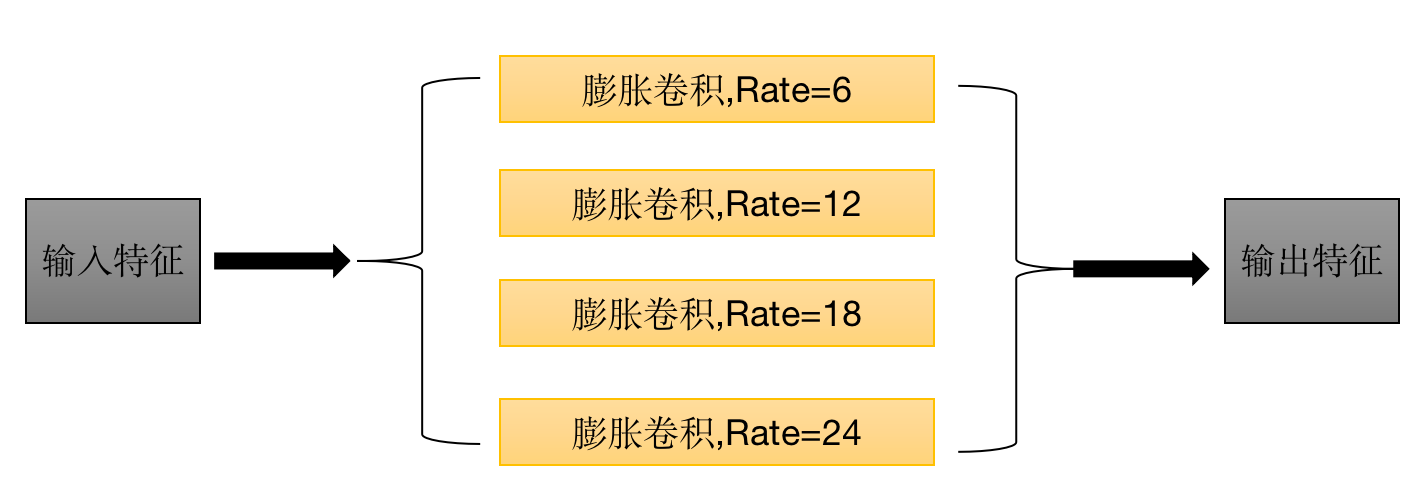
\includegraphics[width=0.65\textwidth]{aspp.png}
    \caption{特征金字塔池化模块}
    \label{aspp}
\end{figure}

\section{渐进残差注意力优化模块}
在得到了提取的特征$\{f_1, f_2, f_3, f_4,  f_5, f_6\}$后,我们通过卷积和反卷积(deconvolution)上采样处理得到了传入侧枝优化网络的特征$\{h_1,h_2, h_3, h_4,  h_5\}$和侧枝网络的输入边缘图$E_1$,其中$E_1$中包含了大量丰富的边缘细节信息,能为后续的优化提供扎实的基础。在侧枝网络中我们将通过渐进残差注意力优化模块去根据的输入特征$h_i$去逐步优化输入的边缘图$E_1$,最终的得到$E_5$。通过渐进残差注意力优化模块,我们能在侧枝网络中将带有丰富细节信息的边缘图和带有丰富上下文 语义信息的高层特征进行有效的结合,达到一个良好的效果。对于每个渐进残差注意力优化模块,接受上一阶段的边缘图{$E_{i-1}$和当前层的特征图$h_i$作为输入,生成当前层的边缘预测结果$E_i$。渐进残差注意力模块又可以分为残差单元和注意力机制部分。

\subsection{深度残差单元}
渐进残差注意力优化模块的第一部分由两个深度残差单元构成,类似的深度残差单元同样也出现了在残差网络中, 我们首先介绍这个模块。对于一个残差小单元来说,可以表述为下面的形式:
\begin{equation}
    y = f(x; W_i) + x
\end{equation}
其中$x$代表残差连接的输入,$y$代表残差连接的输出。$f()$代表残差连接中的卷积层。$W_i$代表残差连击中需要学习的参数。在深度残差单元中,$f(x; W_i)$又两个 卷积核大小为$3 \times 3$的卷积层构成,其中ReLU激活函数在每个卷积后作为对应的激活函数。另一种架构方式为:
\begin{equation}
    y = f(x; W_i) + Conv(x)
\end{equation}
其中$Conv$代表了卷积层,相比第一种结构利用$Conv(x)$代替了$x$,此处$Conv$的主要作用在于统一残差模块中的维度,保证残差模块中维度保持相同。例如对于边缘图输入$E_i \in H \times W \times 1$,$Conv$能够将$E_i$在残差中保持统一的通道数方便后续计算 。整体来看,深度残差单元的计算流程为:
\begin{equation}
    y =  Conv(f(f(x) + Conv(x)) + f(x) + Conv(x))
\end{equation}
在深度残差单元中所有的卷积层的卷积核都设置为$3 \times 3$大小,卷积核个数为256,步长为1。

\subsection{空间注意力机制}
渐进残差注意力优化模块的目标是根据当前较高层的特征去优化上一层得到的边缘预测结果,进一步得到当前层的边缘预测结果。对于第$i$层的渐进残差注意力优化模块,接受$i-1$层产生的边缘预测结果$E_{i-1}$和当前层的视觉特征$h_i$。对于输入的$E_{i-1}$和$h_i$,首先经过一个深度残差单元进一步提取特征,之后模块会将两部分得到的结果特征图进行逐元素的相加,我们将通过深度残差单元最后相加得到的特征表示为$f \in H \times W \times C$。其中H和W代表特征图对应的高和宽,C代表特征图的通道数。

通常来说较低层得到的特征图$E_{i-1}$有着丰富的细节信息和局部信息,而高层得到的$h_i$有全局上下文语义信息。简单通过相加将他们合成一个特征图不是一个最优方案,我们利用注意力机制探寻一种更优的解决方案去结合两部分特征。注意力机制已经被广泛应用在了其他方面并且取得了良好的效果。我们利用视觉注意力机制引导我们更好的融入高层特征的语义信息,指导低层边缘图去除弱边缘和噪点。

给定特征$f \in H \times W \times C$,我们能够通过一个带有偏置项的卷积层和一个softmax激活函数层得到对于特征的一个软注意力特征图(soft attention map)。
\begin{equation}
    g = ReLU(w_{a} \star f + b_{a})
\end{equation}
\begin{equation}
    \label{compute_att}
    {p_{a}(h, w, 1) = \frac{e^{g(h,w, 1)}}{\sum_{\substack{h \in \mathbb{L}}\\ ,w \in \mathbb{L}}  e^{g}(h,w,1)}}
\end{equation}

其中$w_{a}$代表卷积层,$b$代表卷积层的偏差项,ReLU代表激活函数。$g \in \mathbb{R} ^{h\times w{\times 1}}$代表每个通道的总结特征。$\mathbb{L} = \{(h, w)| h = 1, ..., W, w =  1, ..., H\}$代表在总结特征上$g$的所有像素点。对于每个注意力图$p \in \mathbb{R}^{H \times W \times 1}$,能够通过式子\eqref{compute_att}来计算注意图图上的每一个点$(h,w,1)$。 

通过上面的计算我们得到了软注意力特征图$g$,我们能够得到一个新的、经过注意力机制处理之后的特征图为$f_{a}$:
\begin{equation}
    f_{a} =  p_{a} \star f 
\end{equation}
得到$f_{a}$之后,我们会通过两个卷积层去获得最终的优化后的当前层的预测结果,这两个卷积层的作用是用于将特征图进行降维并最终输出为边缘图(edge map)的形式。在具体的实现过程中,softmax之前的卷积层参数为$3 \times 3 \times 256$。最后两层卷积的参数设置为$1 \times 1 \times 21$和$1 \times 1 \times 1$。所有卷积层的步长都设置为1。

\section{网络实现细节和损失函数}
常规的分类任务通常使用交叉熵损失函数。因为边缘检测任务中的数据不平衡问题,我们仿照HED中的做法引入了类别权重用于平衡正负样本,最终使用了类别权重平衡的交叉熵损失函数。损失函数表达式如下:
\begin{equation}
\begin{aligned}
    l(W) = -\gamma \cdot \beta \sum\nolimits_{g_{i} \in G_{+}}\log P(g_{i} = 1 | I ; W) \\
    - (1 - \beta) \sum\nolimits_{g_{i}\in G_{-}}\log P(g_{i} = 0 | I ; W)
\end{aligned}
\end{equation}

其中$I$是输入图片,$G$是输入图片$I$的真值。$\beta$是类别平衡的权重,表达为输入图片上非边缘点个数和总像素个数的比值。由于我们知道输入图片上像素点个数很少,所以$\beta$的值能够给边缘点和非边缘点合理的权重。$g_i$代表输入图片$I$上的像素点。$W$代表网络中的所有参数。$\gamma$是一个超参数,用于进一步平衡正负样本权重。

在训练方法上,同样是采用了深度监督的训练方式,这一训练方式广泛用于边缘检测任务中,有利于梯度更好的回传,取得了良好的效果。

训练采用的数据集是BSDS500和NYUDv2数据集。对于NYUDv2数据集来说,每一个输入图片$I$都有唯一对应的真值标注$G$。而对于BSDS500数据集来说,因为不同人对于边缘的主观认知存在着偏差,如果存在的多人标注同一张图片,会出现不同人的边缘标注的差异。而BSDS500数据集的每一个图片$I$对应了多个(4-7个不等)标注者标注的真值图片,每个人标注的真值都不相同。为了在网络训练过程中给网络一个稳定的真值结果,我们对BSDS500的真值在训练时候做如下处理。

首先对于每一个图片 $I$,我们将它的所有标注进行平均,得到了一个平均标注图,其中像素的值在0-1之间。若值为0,代表该像素点没有被任何一个标注者标注为边缘点。若该像素点的值为1,则代表该像素点被所有标注者都标注为边缘点。但是分类网络需要一个稳定化的分类真值,为了得到一个准确的分类,我们定义规则:如果一个像素点的值大于0.2,即只要该点被一个标注者标注为了边缘点,在网络中我们就认为它是边缘点,对应的真值为1。

采用这样策略的一个原因是考虑到我们的自顶向上的渐进优化网络在渐进优化的过程中,需要一个带有丰富细节信息的边缘图作为初始边缘图。而采用这样的策略,能够尽可能保留所有标注者对应的标注,给后续的优化过程提供丰富的信息。

整个网络采用Tensorflow深度学习框架\citing{Tensorflow}实现,并且采用了在ImageNet\citing{ImageNet}上预训练的残差网络作为提取特征的主干网,并且用预训练的参数进行初始化,有助于网络的加速收敛。网络的学习率设置为$1 \times e^{-6}$, 学习过程中采用了Adam作为训练的优化器。因为训练集合大小原因(在BSDS500和NYUDv2上均做了数据增强),在BSDS500数据集上训练60000次而在NYUDv2上训练80000次。在网络训练过程中,采用了poly的学习率衰减策略,具体的表达式为:
\begin{equation}
    lr = lr \times (1 - \frac{iter}{max\_iter})^{power}
\end{equation}

其中$lr$代表学习率,$iter$代表现在的训练次数,$max\_iter$代表最大训练次数,$power$代表指数,这里我们设置为0.9。

\section{实验设计部分}
这个部分中,将对算法的实际效果进行大量的实验和可视化分析,并且介绍边缘检测的相关公开数据集和评测方法。最后,本节将分析方法的缺点和后续可能的改进。具体的改进工作将在下一节介绍。
\subsection{数据集介绍} 
边缘检测学术界的公开数据集主要是BSDS500数据集\citing{gPB}和NYUDv2数据集\citing{NYUD}。本小节将分别详细介绍两个数据集。

\textbf{BSDS500}数据集全称是来自加州伯克利大学计算机视觉组提出的边缘检测数据集,全称为Berkeley Segmentation Data Set and Benchmarks 500。数据集为当时的边缘检测和图像分割任务提供了一个用于训练和测试的标准数据集,并且为其提供了评测代码用于大家统一进行评测。该数据集是之前BSDS300数据集的扩充,其中包含了300张图片用于训练或验证,也包含了200张图片图片作为测试。每张图片都有4-7个标注员对输入的图像进行标注。数据集的图片可视化结果如图\ref{bsds_dataset}所示。\footnote{BSDS500数据集的可视化展示图例来源于加州伯克利大学的数据集官网,链接:https://www2.eecs.berkeley.edu/Research/Projects/CS/vision/grouping/resources.html }
\begin{figure}[h!]
    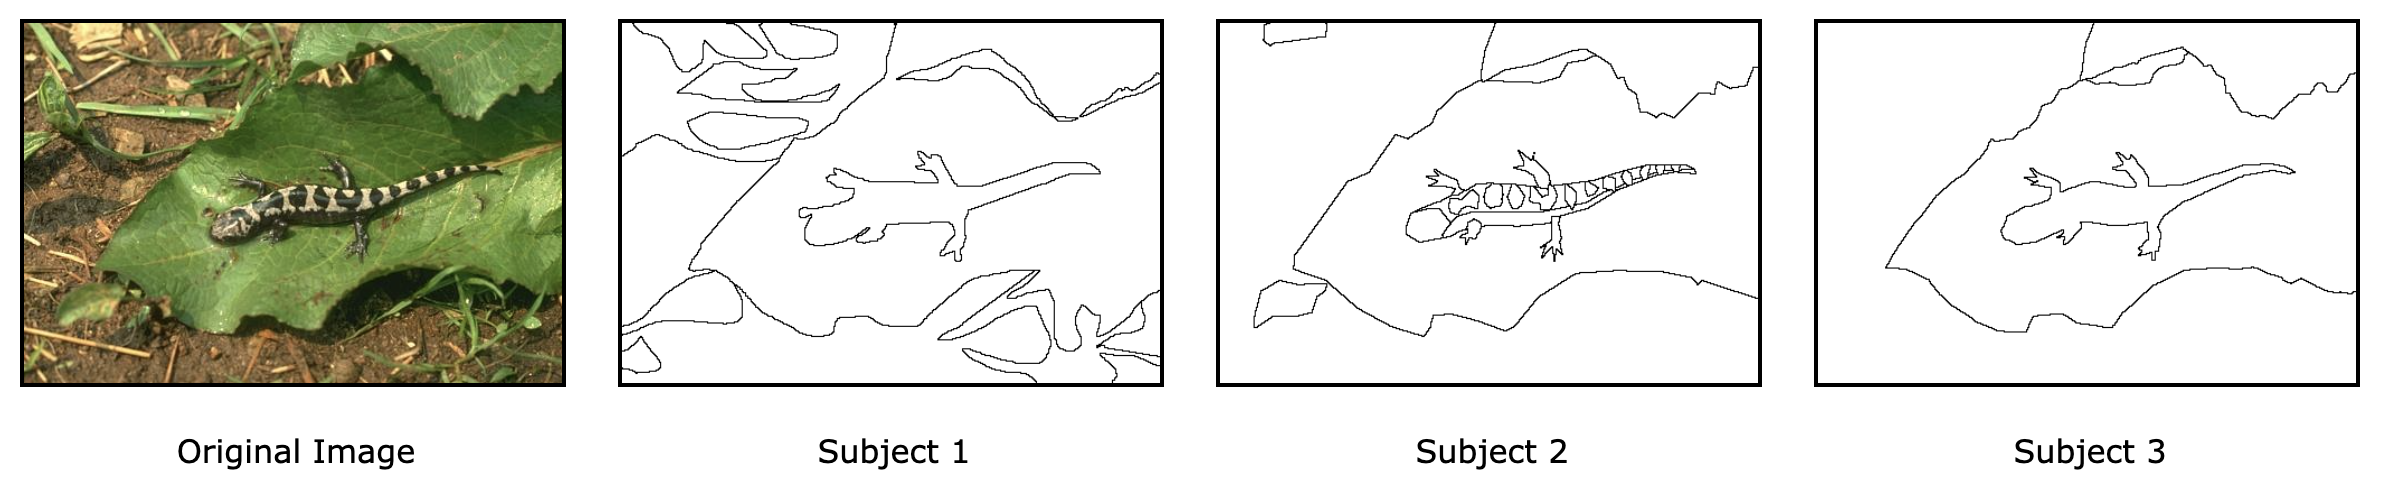
\includegraphics[width=0.95\textwidth]{bsds_dataset.png}
    \caption{BSDS500数据集的可视化展示,图中展示了对应图片和3个不同标注人员进行的标注结果}
    \label{bsds_dataset}
\end{figure}

\textbf{NYUDv2}数据集是一个用于室内场景语义分割和边缘检测的数据集。数据集中包含1449张各种不同室内场景的图片,其中756张图片用于训练,654张图片用于测试。 复杂的室内场景也给了数据集一定的预测难度。数据集中所有图片的分辨率为$560 \times 425$。该数据集的边缘检测标注由语义分割结果的边缘进行生成,所以该数据集的一个输入图片只对应于一个边缘检测真值标注。其中NYUDv2的数据集不仅包含RGB的常规图片,还包含了利用Kinect相机采集得到的深度图片,是一个拥有多模态数据的数据集。对于RGB模态来说,常规的图片尺寸是$H \times W \times  3$,而对于深度模态来说,原始的深度模态的图片尺寸为 $H \times W \times  1$。我们常常将对应的深度图片转化为和RGB图片同样尺寸大小的HHA图片。HHA图片是将深度图片中的深度信息分别编码为水平距离、和水平地面的高度、和重力方向之间的夹角三个通道的信息得到的图片,构由此成了$H \times W \times 3$的网络输入。 最后的预测结果也常常是将两个模态输入之后得到的预测结果进行平均,得到最终的预测结果。而深度模态的结果能够帮助网络相比单独的RGB图片输入得到更好的预测结果,因为深度图片(HHA图片)提供了2D RGB图片中所包含的丰富的几何位置信息,网络充分结合和利用这些几何信息能够让网络相比单独2D RGB图片的输入产生更好的结果。 NYUDv2的可视化结果如图所示,通过对语义分割的标注进行连通区域区域的边界提取处理便能得到对应的边缘图。\footnote{NYUDv2数据集可视化整理来自数据集官网,链接为: \url{https://cs.nyu.edu/~silberman/datasets/nyu_depth_v2.html }}
\begin{figure}[h!]
    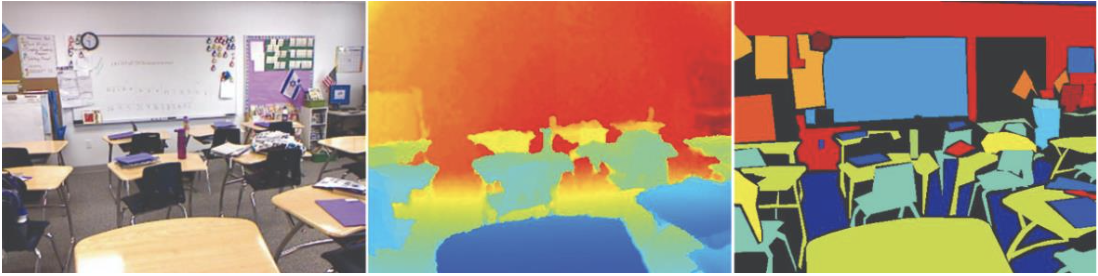
\includegraphics[width=0.95\textwidth]{nyud_dataset.png}
    \caption{NYUDv2数据集的可视化展示,包含了RGB图片,深度图片和对应的语义分割标注。将语义分割标注处理出区域边界就可以得到边缘标注}
    \label{nyud_dataset}
\end{figure}

\subsection{评测指标介绍}
边缘检测网络的评价指标主要有3个,可以区分为全数据集最优尺寸(optimal dataset scale, ODS),图片最优尺寸(optimal image scale, OIS),和平均准确率(average precision, AP)。其中ODS代表整个数据集在最后评测时的二值化时采用统一的最优的阈值,OIS代表了整个数据集在最后评测之时对于数据集中的每张图片采用一个最优的阈值,平均准确率AP代表PR曲线下的面积,为不同阈值下的准确率的平均值。在最后的评测之前需要经过非极大值抑制(non-maximum suppression, NMS)将生成的粗边缘变细之后进行评测。

\subsection{数据增强处理}
边缘检测的数据集中训练集样本数量太少,例如BSDS500数据集中只有300张训练集,而NYUDv2数据集中也仅仅只有765张训练集图片。这么少的训练集对网络训练很容易造成过拟合现象,严重影响网络的泛化能力,所以我们对训练集做了数据增强。

对于BSDS500数据集,我们采用了如下数据增强策略:对于每一张图片,我们分别将其缩放为原来的0.5倍和1.5倍,使得数据规模变为原来的3倍。在不同数据尺寸的基础上,我们对每种数据尺寸下的每张图片从0度到337.5度进行了16个角度(22.5, 45, 67.5, 90, ...,337.5)的旋转,并且裁切旋转后的最大内接矩形为最后的旋转图片,将数据规模扩大为原来的48倍;除此之外,我们还对每种数据尺寸下、每个旋转角度下的图片进行水平方向的翻转,最终扩张为原训练集尺寸的96倍,最后达到了28800张训练集图片。

对于NYUDv2数据集来说,我们同样也做了大量数据增强以满足深度神经网络的训练需求:我们对同样也将其缩放为原来的0.5倍和1.5倍。同时在上面的基础上,我们将图片旋转为90,180,270三个角度,并且对每种角度下的图片都做了水平翻转。通过NYUDv2上的数据增强操作,我们能够将数据集扩充为原来的24倍,最终达到18096张训练集合图片,能够满足网络的训练需求。

通过数据增强处理,我们能够很大程度上避免过拟合问题,也加速了网络的收敛,显著提高了网络的泛化性能,由此能够显著提升网络在测试集上的效果。
\subsection{网络消融实验}
在这个小节中,我们将对网络中的各个模块进行消融实验对比和分析,并证明我们网络中各个模块的有效性。网络中的所有消融实验都是在BSDS500数据集上进行的。

我们将首先分析膨胀卷积和特征池化金字塔结构引入对边缘检测结果造成的影响。我们对膨胀卷积和特征池化金字塔结构进行消融实验。
\begin{table}[h!]
	\begin{center}
		\caption{关于膨胀卷积和特征池化金字塔结构的消融实验}
		\label{tab:ac_aspp}
		\begin{tabular}{l|c|c|c}
			\toprule % <-- Toprule here
			\textbf{方法} & \textbf{ODS} & \textbf{OIS} & \textbf{AP}\\
			\midrule % <-- Midrule here
			我们的模型 (w/o AC+ASPP) & 0.788&0.801&0.817\\   
			我们的模型 (w/AC) & 0.798 & 0.815 &0.824\\
			我们的模型 (w/AC+ASPP) & \textbf{0.805} &\textbf{0.819} & \textbf{0.851}\\
			\bottomrule % <-- Bottomrule here
		\end{tabular}
	\end{center}
\end{table}

通过表\ref{tab:ac_aspp}可以发现膨胀卷积和特征池化金字塔结构在网络中起到了关键的作用。表格中膨胀卷积缩写为AC,而特征池化金字塔结构缩写为ASPP。图中表明特征池化金字塔结构对应网络在ODS、OIS和AP上分别有1\%、1.4\%和0.7\%点的提高。而在特征池化金字塔结构结构的基础上再结合膨胀卷积家又能带来0.7\%, 0.4\%, 2.7\%的点数提高。

接着我们探索了我们提出的自底向上的渐进优化网络的效果。为了方便对比,我们利用了类似HED结果的网络结果作为我们的基线(表\ref{tab:CRA}中的Baseline),具体的实验结果如下:
\begin{table}[h!]
	\begin{center}
		\caption{自底向上的渐进优化网络的消融实验对比效果}
		\label{tab:CRA}
		\begin{tabular}{l|c|c|c}
			\toprule % <-- Toprule here
			\textbf{方法} & \textbf{ODS} & \textbf{OIS} & \textbf{AP}\\
			\midrule % <-- Midrule here
			基线方法 (类似HED的结合方法) & 0.799&0.814&0.758\\   
			我们的方法 (渐进优化-不含注意力机制) & 0.761 & 0.780 &0.801\\
			我们的方法  (渐进优化-包含注意力机制) & \textbf{0.805} &\textbf{0.819} & \textbf{0.851}\\
			\bottomrule % <-- Bottomrule here
		\end{tabular}
	\end{center}
\end{table}

表中的结构证明了我们提出的自底向上的渐进优化网络的作用,提出渐进优化网络能够显著提高网络的平均准确率值(AP),而配合空间注意力机制能够达到相比基线方法更好的效果。相比基线方法,我们提出的网络能够在ODS、OIS和AP指标上分别高出0.6\%, 0.5\%和9.3\%,达到了良好的效果,证明了渐进优化注意力方法的有效性。

同时我们还探索了深度监督对于我们网络训练的影响,在HED的对比实验中可以发现,深度监督能够明显提高网络的训练效果,加速网络收敛。我们同时也探索了深度监督的训练方法在我们的网络中的作用。
\begin{table}[h!]
    \begin{center}
        \caption{深度监督的消融实验效果}
        \label{tab:deep_supervision}
        \begin{tabular}{l|c|c|c}
            \toprule % <-- Toprule here
            \textbf{方法} & \textbf{ODS} & \textbf{OIS} & \textbf{AP}\\
            \midrule % <-- Midrule here
            我们的模型(不使用深度监督) & 0.807&0.822&0.832\\   
            我们的模型(使用深度监督) & \textbf{0.805} &\textbf{0.819} & \textbf{0.851}\\
            \bottomrule % <-- Bottomrule here
        \end{tabular}
    \end{center}
\end{table}
从表\ref{tab:deep_supervision}我们可以发现在指标上深度监督对我们模型的影响不是很大,这也说明了我们的残差网络的设计能够很好的避免梯度消失的问题,有利于梯度的回传。而深度监督的可视化结果如图\ref{deep_supervision}所示,从可视化结果来看深度监督能够更好的去除物体内部的细节纹路,而具体是否采用可以看使用者的需求而定。两者都能谁先一个较好的效果,一个更偏向整体,一个更偏向细节。
\begin{figure}[h!]
    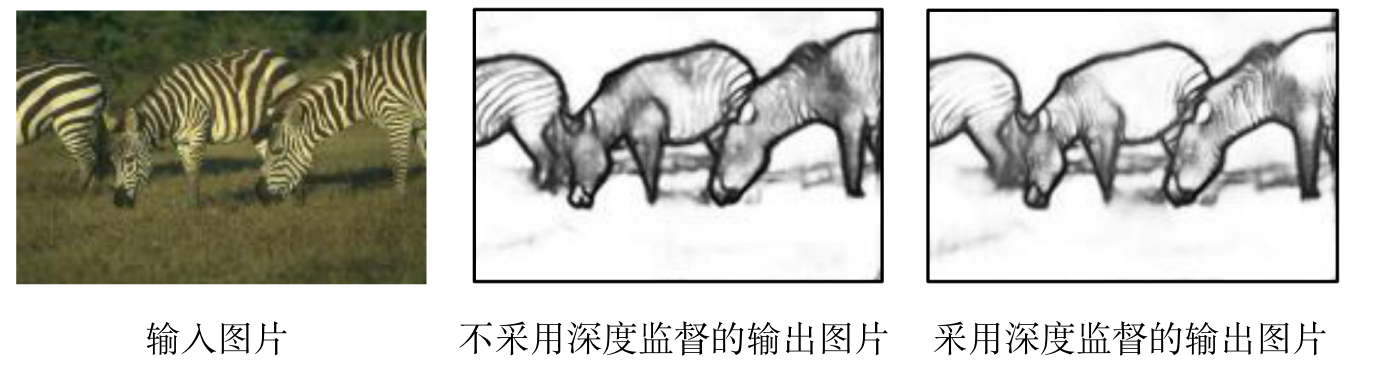
\includegraphics[width=0.95\textwidth]{deep_supervision.png}
    \caption{深度监督训练效果的可视化}
    \label{deep_supervision}
\end{figure}


在表\ref{tab:feature-channel}中,我们对侧枝网络中的特征维度进行了参数敏感度分析,因为残差主干网络的特征维度较大,我们选择了64、128、256和512几个维度进行参数的探究。从表\ref{tab:feature-channel}中可以发现256作为网络一个合适的特征维度,能够取得最好的结果。分析其中的原因:可能是因为较小的特征维度例如64和128,在对残差网络提取的特征维度(256, 512, 1024, 2048)降维的过程中,会损失太多的信息;同时较小的特征维度也没有充分的特征表达空间,影响了最终的效果。而高维度的特征不仅会耗费更大的资源,同时,对于边缘检测任务,过大的网络参数量容易造成网络过拟合。
\begin{table}[h!]
    \begin{center}
        \caption{网络侧枝中特征维度对于最终效果的影响}
        \label{tab:feature-channel}
        \begin{tabular}{l|c|c|c}
            \toprule % <-- Toprule here
            \textbf{特征维度} & \textbf{ODS} & \textbf{OIS} & \textbf{AP}\\
            \midrule % <-- Midrule here
            64 & 0.799&0.803&0.817\\   
            128 & 0.802 &0.807 & 0.823\\
            256 &\textbf{0.805}&\textbf{0.819}&\textbf{0.851}\\  
            512 & 0.803&0.817&0.842\\    
            \bottomrule % <-- Bottomrule here
        \end{tabular}
    \end{center}
\end{table}

根据表\ref{tab:cost}中的复杂度分析可以发现,在优化之后的侧枝网络的计算资源消耗很低,极大了增加了网络了运行效率。对应的时间复杂度在Ubuntu 16.04, CUDA 9和Nvidia 1080Ti单卡上进行测试。
\begin{table}[h!]
    \begin{center}
        \caption{网络的计算资源和运行时间复杂度分析}
        \label{tab:cost}
        \begin{tabular}{c|c|c}
            \toprule % <-- Toprule here
            \textbf{主干网络FLOPs} & \textbf{全部网络FLOPs} & \textbf{FPS}\\
            \midrule % <-- Midrule here
            18.23G&41.2G&10\\    
            \bottomrule % <-- Bottomrule here
        \end{tabular}
    \end{center}
\end{table}


\subsection{和其他方法的对比}
我们在两大公开数据集BSDS500和NYUDv2上和其他当时学术界的先进方法做了比较,证明了我们方法的先进性。其中BSDS500上的效果如表\ref{tab:bsds}所示,而在NYUDv2上的效果如\ref{tab:nyud}所示。从结果上来看我们的方法超过了当时学术界的主流方法,达到了学术界的先进水平。其中在表\ref{tab:bsds}中灰色字体的方法使用了额外的数据集进行训练,这里我们不做比较。
\begin{table}[h!]
    \begin{center}
      \caption{在BSDS500数据集上和其他方法的比较结果}
      \label{tab:bsds}
      \begin{tabular}{l|c|c|c}
        \toprule % <-- Toprule here
        \textbf{方法} & \textbf{ODS} & \textbf{OIS} & \textbf{AP}\\
        \midrule % <-- Midrule here
        Canny\citing{Canny} &0.611 & 0.676 & 0.580\\
        EGB\citing{EGB}  & 0.610 & 0.640 & 0.560\\
        Mean Shift\citing{MeanShift}  & 0.640 & 0.680 &0.560\\
        gPb-UCM\citing{gPB}  & 0.726 &0.760 &0.727\\
        Sketch Tokens\citing{lim2013sketch}  & 0.727 & 0.746 & 0.780\\
        MCG\citing{traditional_5} &0.747&0.779&0.759\\
        SE\citing{traditional_1} &0.746&0.767&0.803\\
        OEF\citing{OEF} &0.749&0.772&0.817\\
        \hline
        DeepContour\citing{DeepContour} &0.756&0.773&0.797\\
        DeepEdge\citing{DeepEdge}  & 0.753&0.772&0.807\\
        HFL\citing{HFL}  & 0.767&0.788&0.807\\   
        
        HED\citing{HED} &0.788&0.808&0.840\\
        CEDN\citing{CEDN} &0.788&0.820&0.834\\
        
        COB\citing{COB} &0.793&0.820&0.859\\ 
        \textcolor{gray}{RCF\citing{RCF}} &\textcolor{gray}{0.811}&\textcolor{gray}{0.830}&\textcolor{gray}{0.839}\\
        \hline
        我们的方法  & 0.805&0.819&0.851\\
        我们的方法-多尺度图片输入 &\textbf{0.819}&\textbf{0.835}&\textbf{0.862}\\
        \bottomrule % <-- Bottomrule here
      \end{tabular}
    \end{center}
  \end{table}

  \begin{table}[h!]
	\begin{center}
		\small
		\caption{在NYUDv2数据集上和其他方法的比较结果}
		\label{tab:nyud}
		\begin{tabular}{l|c|c|c}
			\toprule % <-- Toprule here
			\textbf{方法} & \textbf{ODS} & \textbf{OIS} & \textbf{AP}\\
			\midrule % <-- Midrule here
			OEF\citing{OEF} &0.651&0.667&-\\
			gPb-UCM\citing{gPB}  & 0.632 &0.661 &0.562\\
			gPb+NG \citing{gupta2013perceptual}&0.687&0.716&0.629\\
			SE \citing{traditional_1}&0.685&0.699&0.679\\
			SE+NG+ \citing{gupta2014learning}&0.710&0.723&0.738\\ 	\hline
			
			
			HED(HHA) \citing{HED}&0.682&0.695&0.702\\
			HED(RGB) \citing{HED}&0.720&0.734&0.734\\
			HED(RGB + HHA) \citing{HED}&0.746&0.761&0.786\\
			RCF(HHA) \citing{RCF}&0.705&0.715&{{0.693}}\\
			RCF(RGB) \citing{RCF}&0.729&0.742&{{0.650}}\\
			RCF(RGB + HHA) \citing{RCF}&0.757&0.771&0.748\\
			\hline
			我们的方法 (HHA)&0.679&0.697&0.701\\
			我们的方法 (RGB)&0.756&0.771&0.765\\
			我们的方法 (RGB+HHA)&\textbf{0.762}&\textbf{0.781}&\textbf{0.797}\\
			\bottomrule % <-- Bottomrule here
		\end{tabular}
	\end{center}
\end{table}
我们同时绘制了BSDS500数据集和NYUDv2数据集上的PR曲线图来展示我们方法的先进性。在PR图中,曲线位于上方的方法有着更好的效果。图\ref{pr_bsds_nyud}分别展示了BSDS500和NYUDv2上的PR曲线图。从图中可以发现我们的曲线位于其他方法的上方,说明了我们方法的效果超过了之前学术界的其他边缘检测方法。
\begin{figure}[h!]
    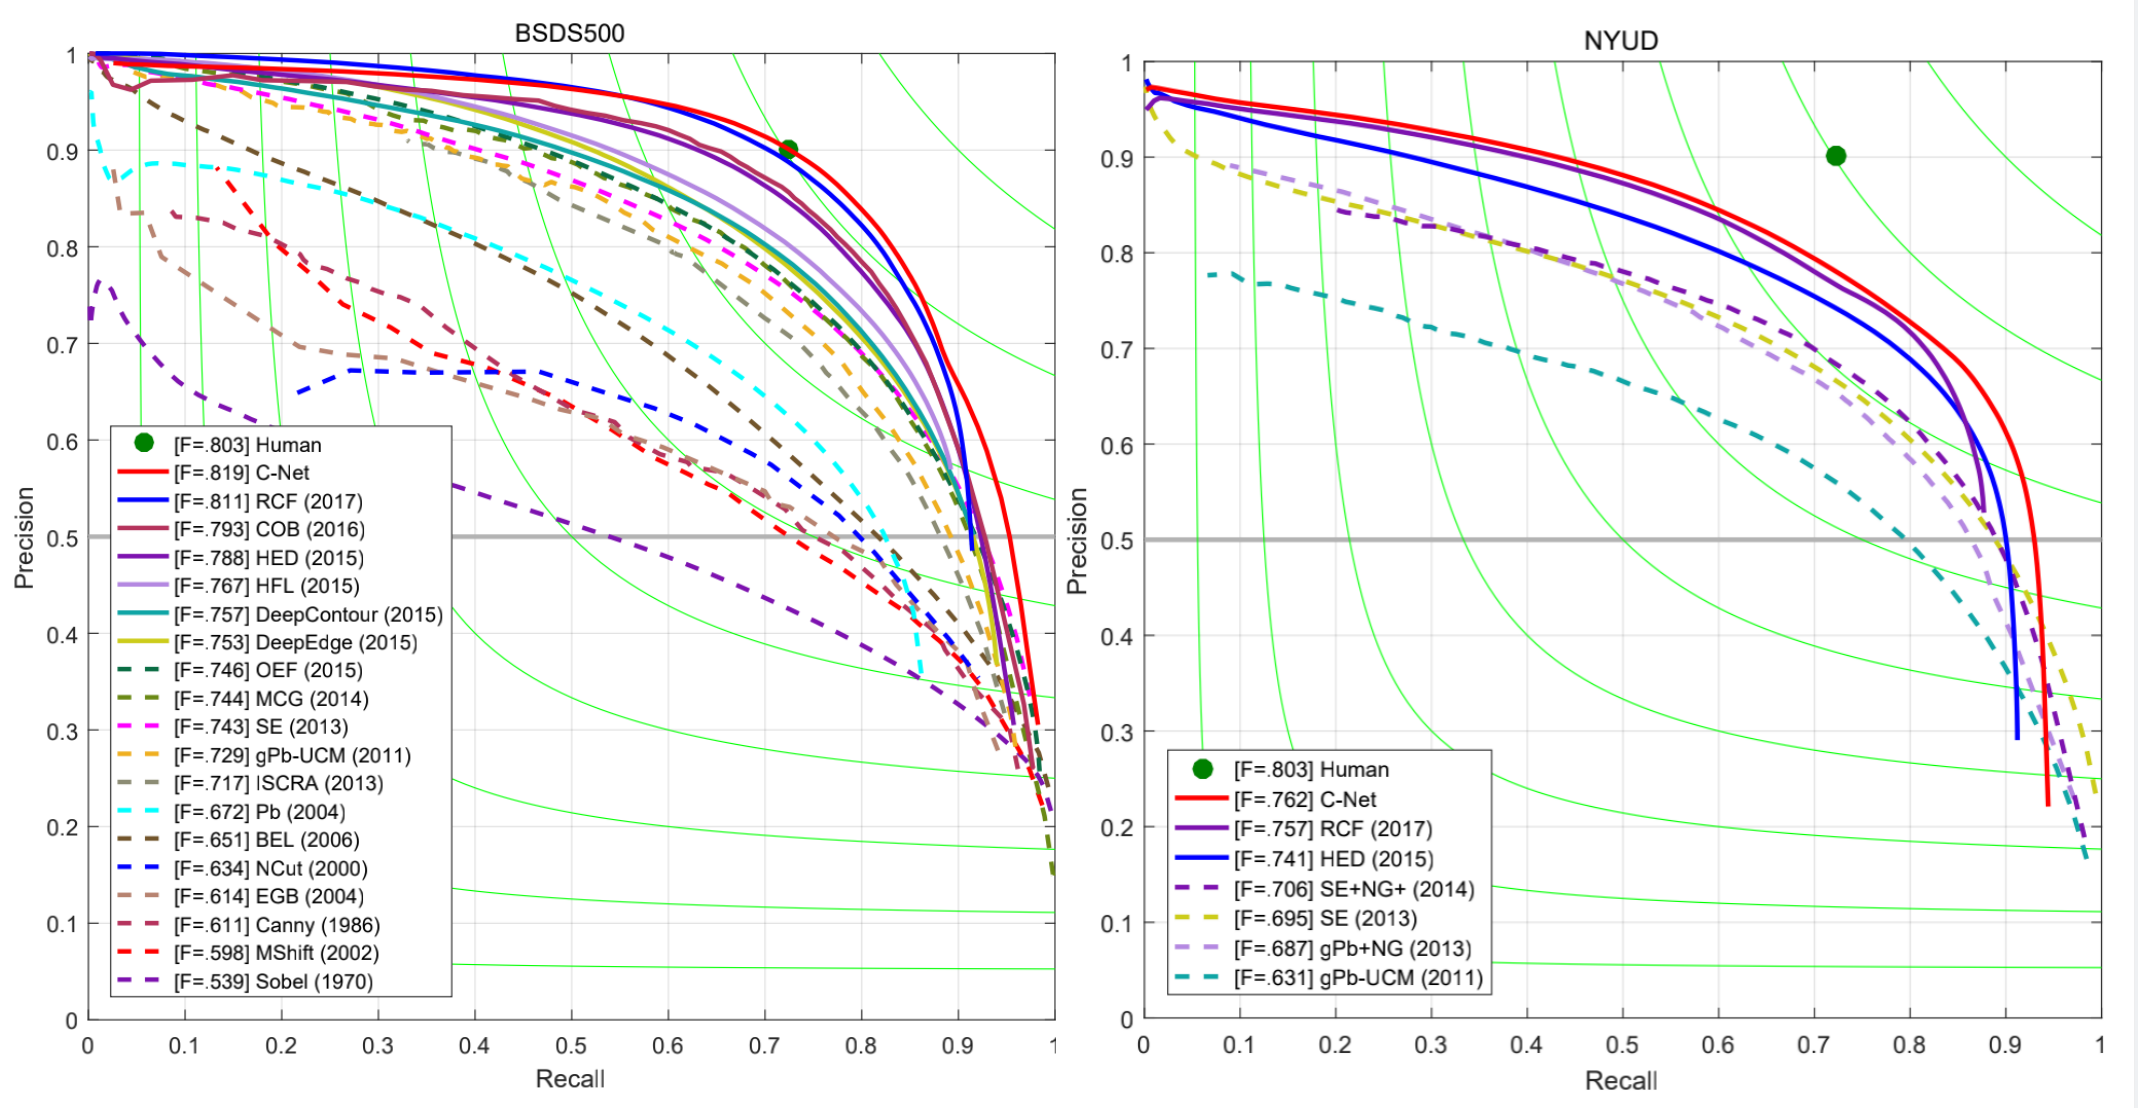
\includegraphics[width=1.0\textwidth]{bsds_nyud_pr.png}
    \caption{在BSDS500数据集和NYUDv2数据集上的PR曲线图}
    \label{pr_bsds_nyud}
\end{figure}




\subsection{可视化结果展示}
本节我们展示了我们的方法不同层的输出可视化结果图\ref{visual_side_out},从可视化中可以发现我们的方法能够逐渐产生准确、高质量的边缘结果。浅层的边缘图能够在网络中被逐渐优化为高质量的高层边缘预测结果图。
\begin{figure}[h!]
    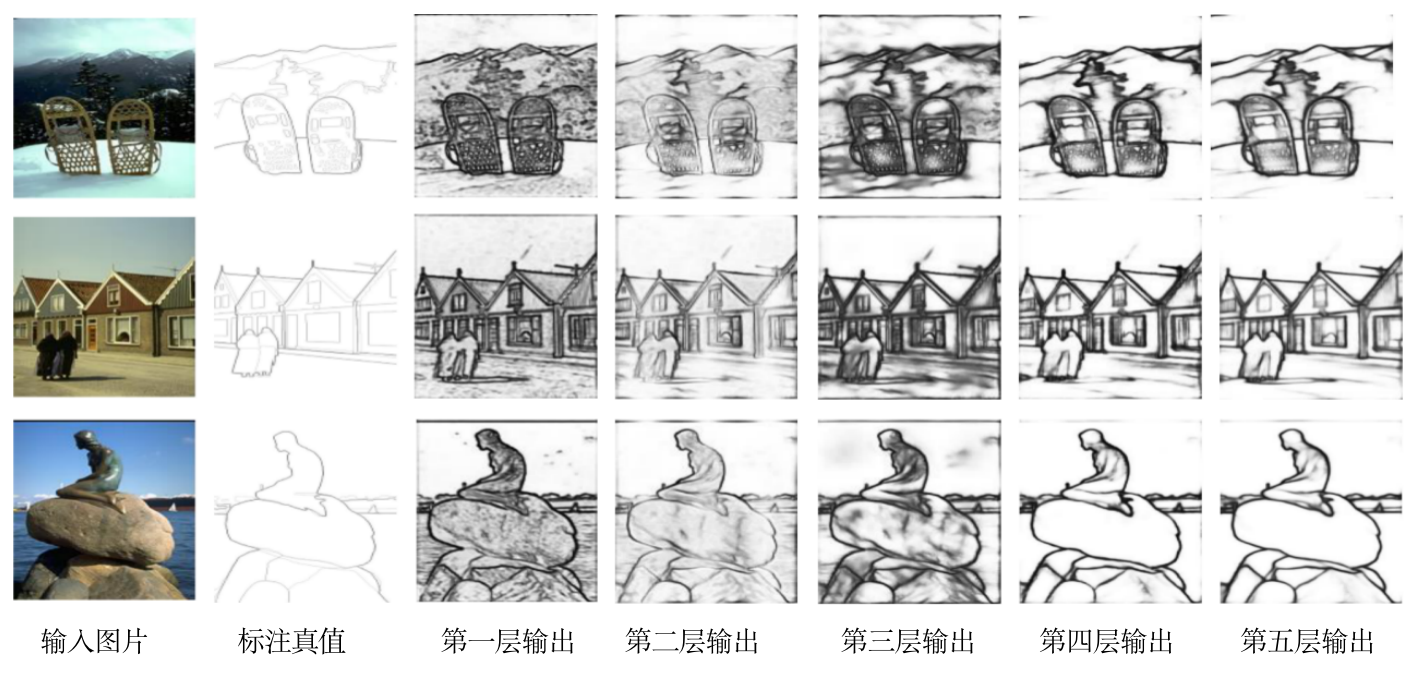
\includegraphics[width=0.95\textwidth]{visual_side_out.png}
    \caption{方法的输出可视化结果图,包含中间层输出和最后输出}
    \label{visual_side_out}
\end{figure}
\subsection{方法的缺点和未来工作}
本节提出的方法能够在两大公开数据集BSDS500和NYUDv2上超过当时所有的边缘检测方法,达到了学术界的先进水平。从可视化结果我们也可以发现我们提出的自底向上的渐进优化边缘检测算法能够通过对高层语义特征的获取逐步改善边缘检测的效果。但是方法仍然存在一些问题:由于我们在进入侧枝网络之前,对于所有进入侧枝网络的特征,我们都利用了反卷积的上采样模块将特征图采样到输入图片大小。而侧枝网络中的残差网络和高分辨率的特征图会消耗大量的计算资源,这导致整体网络的运行速度受到影响。针对网络计算量过大的问题,我们需要在接下来的网络设计中考虑到这一点。 

同时我们可以发现膨胀卷积和特征金字塔网络网络对于边缘检测任务来说具有良好的效果。对于膨胀卷积,我们可以作为一个常规的模块应用在后续边缘检测任务的设计之中。而对于特征金字塔网络,在本节的网络设计中我们将其设计为主干网络的延伸部分,用来对主干网络提取的特征$f_5$进行特征的进一步增强得到了多个感受野合成的特征$f_6$。而我们在后续网络的设计中可以充分利用类似特征池化金字塔网络的金字塔结构对特征进行增强提取,达到更好的效果。

自顶向下的渐进注意力增强网络已经在边缘检测上取得了良好的效果,这引导我们继续尝试更好的多尺度特征结合方法,以求达到对多尺度特征的有效融合,这些内容的思考将会反应在下一章的工作中,有助于我们引出下一章的改进方法。

不过本方法虽然有着以上的缺陷,不过也为后续在边缘检测上的探索打下了坚实的基础。
\section{本章小结}
本章我们提出了基于自底向上的渐进网络优化边缘检测算法,在两大公开数据集上均取得了良好的效果,超过了当时学术界的其他边缘检测算法。并且我们通过大量充分的消融实验证明了我们提出的模块在边缘检测任务中的有效性。对渐进网络中的不同层输出边缘图的可视化 结果也表明了我们的算法能够有效地对网络中的边缘进行逐层的优化,最后达到良好的效果。

本章提出的算法仍然存在着计算量过大等问题,但是一些模块在边缘检测上的良好效果也能够引发我们新的思考,为后续的边缘检测研究打下坚实的基础。这也是未来工作的需要解决和继续改善的问题。




\chapter{双向特征优化的边缘检测算法}
边缘检测算法已经在深度学习时代得到了快速的发展。由于卷积神经网络对于图片多层次特征的提取效果,已经被广泛应用在了边缘检测网络中,并且取得了良好的效果。其中HED算法奠定了深度学习时代端对端进行边缘检测的基本思路和框架,大量的算法在HED网络的基础上进行修改进而被提出。而我们可以将过去的算法大概分为三种:HED结构、自底向上的结构、自顶向下的结构。其中HED结构中代表性的方法有HED\citing{HED}、RCF\citing{RCF}等。自顶向下的结构中代表性的方法有CED\citing{CED}、AMHNet\citing{AMHNet}。而自底向上的结构中代表方法有RDS\citing{RDS},和我们在上一章节中介绍的基于自底向上的渐进优化边缘检测算法。其中不同的方法可以通过图\ref{different_structure}来表达:
\begin{figure}[h!]
    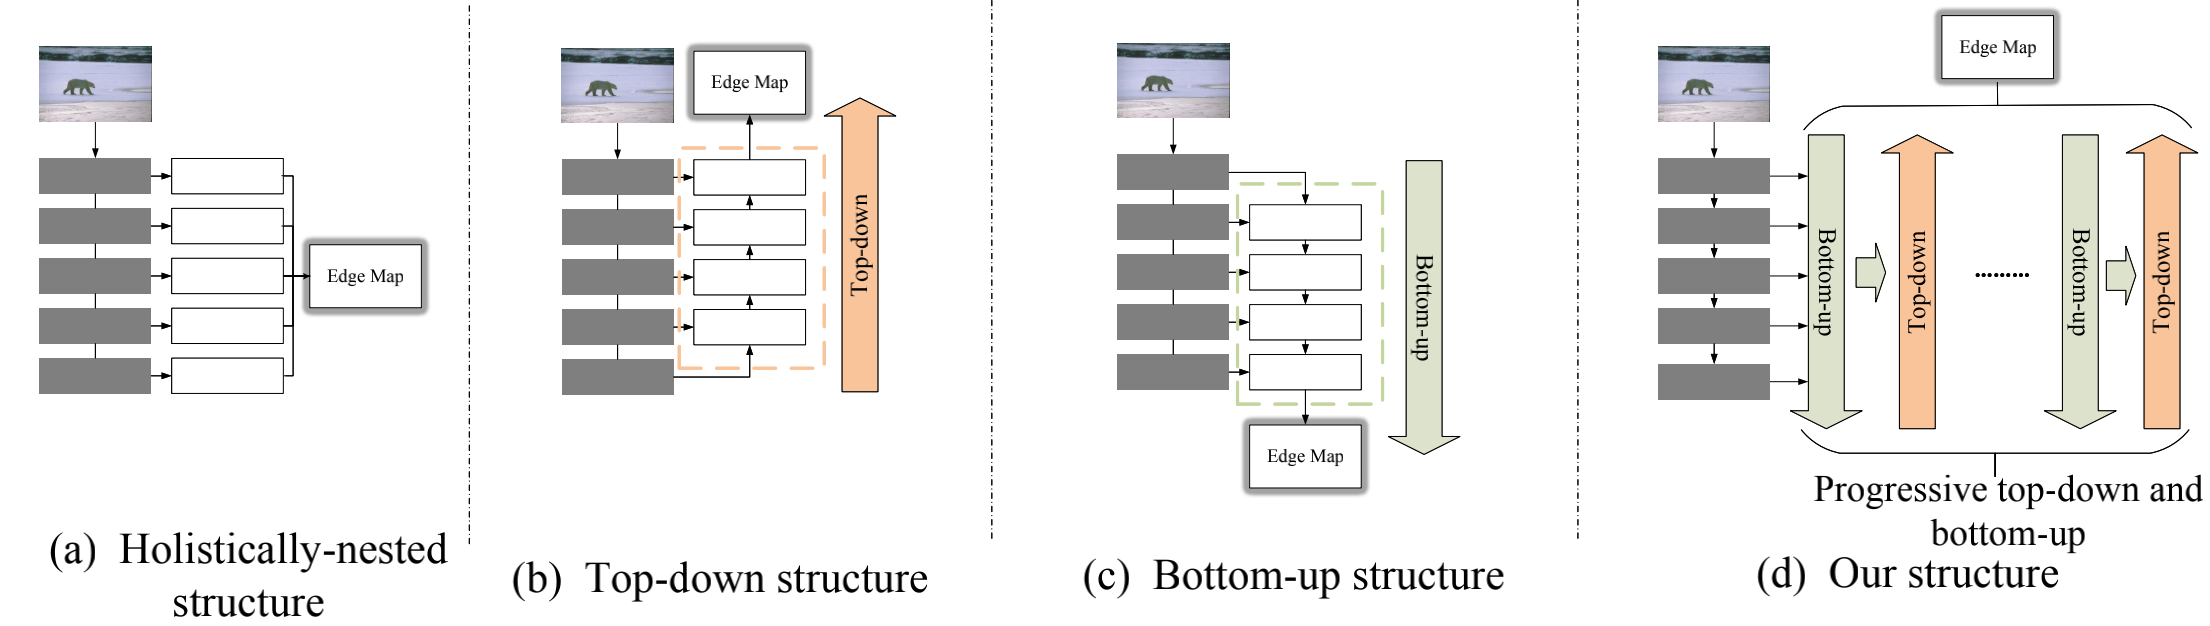
\includegraphics[width=1.0\textwidth]{different_structure.png}
    \caption{边缘检测中不同类型的深度学习方法网络框架结构示意图。(a)代表HED的结构,每层特征独立处理最后通过线性加权在一起得到最终结果;(b)自顶向下的特征优化网络,特征从网络高层到低层逐层结合优化; (c)自底向上的特征优化网络;(d)我们提出 的双向特征优化网络,能充分利用双向弥补单向网络的缺点,达到更好的效果}
    \label{different_structure}
\end{figure}

其中HED结构从主干网络的五个阶段上提取到多层次的特征获取对应的侧枝上的输出,之后通过一个线性加权操作得到最终结果。通过观察我们能发现,低层特征通常包含大量的细节信息同时伴随着大量的噪点,而高层次的特征通常包含丰富的语义信息但是因为主干网络中的池化层的原因,造成高层次特征的分辨率较低,边缘表达的可视化比较模糊。这样多层次的特征能够在网络中达到互补的作用。然而多尺度特征的线性组合
并不能充分挖掘多层次边缘特征之前复杂的关系从而达到良好的组合效果,因为各个侧枝输出是独立的。

后续有的基于深度学习的边缘检测算法采用了自顶向下的架构模式,这一架构模式的思想来自于语义分割的经典方法U-Net\citing{UNet}中。在自顶向下的架构模式中,带有语义信息的高层特征逐渐传递到低层特征中进行有效的结合。通过这种架构方式,在高层边缘表达中丢失的细节信息将被逐渐找回;而模糊的高层特征图将在这个流程中被逐渐优化,得到最终的结果。

基于自底向上的架构模式,和自顶向下的架构有相反的特征传递方向,但是他们都有着类似的思想,都是通过低层或者高层的逐层融合达到良好的多层次 特征融合的效果,我们上一章提出的方法就是采用了自底向上的网络架构模式。 对于理想情况下的单向传递例如自底向上的架构,理想的情况是,带有丰富细节信息的低层特征在传递过程中,细节信息都能够被继承保留而冗余的、错误的信息能够逐渐去除。然而在实际情况中,对于单向的自底向上的架构,低层次特征带有的丰富的细节信息会在不断和高层次特征进行结合的 过程中被遗忘或削弱,对最后的边缘预测结果造成无法修正的影响。同样的问题也会出现在自顶向下的单向网络架构中。我们我们思考如何充分利用自顶向下和自底向上两种网络架构之间的优势,让他们达成一种互补的关系从而弥补单向网络中的缺点,从而提高特征的层次性,恢复丢失的信息,从而达到更好的边缘预测结果。为此,我们提出了本章的双向特征优化算法,其中连续自顶向下和自底向上的网络结构能够为建立一个长距离的信息通路使得多层次的信息更好的流通。

在这一章中,我们主要关注在两个主要的问题上:(1)如何设计一个能够有效结合层次性信息的统一的网络;(2)如何实现不同阶段不同层之间有效的信息传递从而提高边缘检测预测的结果。为了解决这些问题,我们提出了本章的方法,通过结合自底向上和自顶向下的信息传递来达到更好的预测结果。在双向特征优化网络中,自底向上的模块能够逐渐去除细节和尖锐的边缘进而得到准确的边缘预测结果;而自顶向下的模块能够通过重新获取带有丰富空间信息和细节信息的低层次特征从而对自底向上流程中被遗忘的细节进行修正。两者互补能够达到更好的边缘检测效果。
 
同时在网络的设计过程中,我们充分考虑到了上一章提出的网络计算量过大的问题,我们在网络设计过程中的各个细节都尽力减小相关的计算量。例如我们会对主干网络提取的多尺度特征进行降维进而减小后续双向特征优化网络的计算量;我们也发现在侧枝网络中的深度残差单元在我们设计的网络中的效果并不明显,但是会增大很多的计算量,所以我们在双向的侧枝网络中移除了对应的深度残差单元,而采用注意力机制引导的简单相加。

同时膨胀卷积和特征池化金字塔网络已经在上一章的实验中证明了他们在边缘检测任务中的作用,在这一章提出的改进方法中,我们同样使用膨胀卷积替代了主干网络中的一些卷积层,同时充分利用了类似的金字塔网络对特征的强化作用,在每个阶段都引入了类似的金字塔网络,实验证明达到了很大的效果提升。具体的细节内容将在本章后续讲述。

同时在双向网络中,观察到生成的特征中不同的通道的信息对于其他层次来说重要性不再相同,可能有的特征通道中会存在冗余特征(如图\ref{different_channel}所示),所以我们同样使用了注意力机制引导的每个阶段的特征合成模块,此时我们使用了基于通道的注意力机制用于过滤传递中的信息,提取其中的重要部分,同时去除其中的冗余部分。针对网络边缘细化的问题,除去带权重的二分类交叉熵损失函数,我们额外引入了Dice损失函数作为带权重二分类交叉熵函数的补充,Dice损失函数被广泛应用在正负样本不平衡的图像分割算法中\citing{huang2018robust}。
\begin{figure}[h!]
    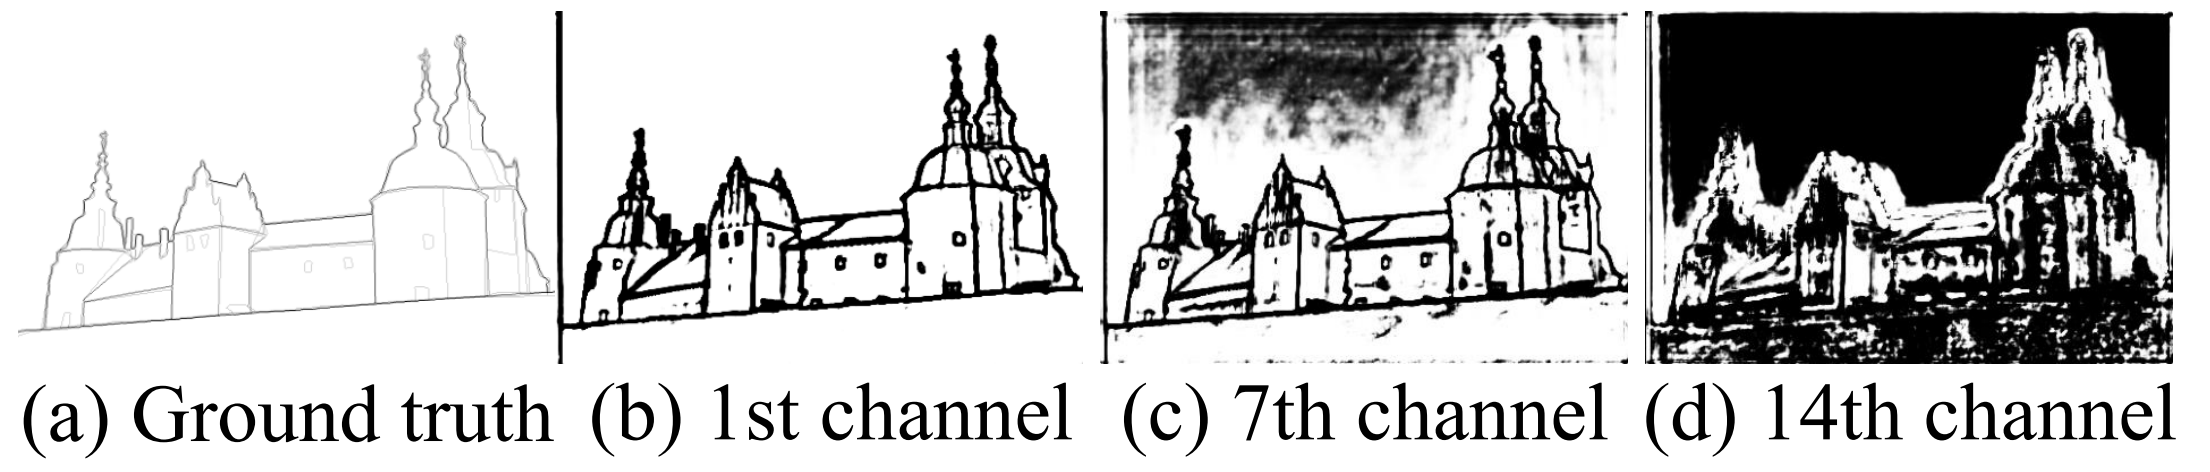
\includegraphics[width=1.0\textwidth]{different_channel.png}
    \caption{生成特征图的不同通道可视化结果,不同的通道中含有不同重要性的信息。我们对于当前特征来说发现第一个通道会比其他通道拥有更丰富和更准确的信息,进而在通道注意力机制中,网络会自动化地给予第一个通道更多的权重}
    \label{different_channel}
\end{figure}

总的来说,我们的贡献点如下:

1)我们根据单向传递网络中可能遇到的问题,结合单向的自底向上和自顶向下侧枝网络,进而提出了双向特征优化的边缘检测网络,在边缘检测上达到了良好的效果,并且相比上一章的方法极大减小了网络的计算量。

2)我们综合考虑了上一章网络遇到的问题,通过网络多处模块的设计极大减小了网络消耗的计算资源;并且在网络中充分利用了特征金字塔网络,使得网络达到了精度和速度两方面的提高。

3) 我们探索了通道注意力机制在边缘检测中的效果,并且将通道注意力机制用于在特征结合时对信息进行过滤和整合,实验证明了相关的注意力机制对边缘检测的效果

4)我们为了让网络预测的边缘变得更加细,引入了Dice损失函数。可视化的结果证明了Dice损失函数对于细化边缘的效果。

5) 我们的网络在两大公开的基准数据集BSDS500和NYUDv2上都超过了学术界的其他方法,证明了我们提出的方法在边缘检测上的有效性。

\section{双向特征优化网络算法}
在本节中,我们将详细介绍我们提出的双向特征优化的边缘检测网络模型,在网络模型中我们同时引入了自底向上和自顶向下的网络结构模型。并且介绍提出其中的网络模型模块和设计, 同时介绍我们网络训练的损失函数和训练模式。

给定输入图片$I \in \mathbb{R}^{H \times W \times 3}$, 网络的目标是预测一个准确的边缘图$E_f\in \mathbb{R}^{H \times W \times 1}$。网络的具体结构如图\ref{framework2}所示。其中可以主要分为4个部分:金字塔特征提取网络、自底向上特征传递模块、自顶向下特征传递模块和注意力机制引导的特征合成模块,在下面我们将详细介绍4种模块的具体细节设计。
\begin{figure}[h!]
    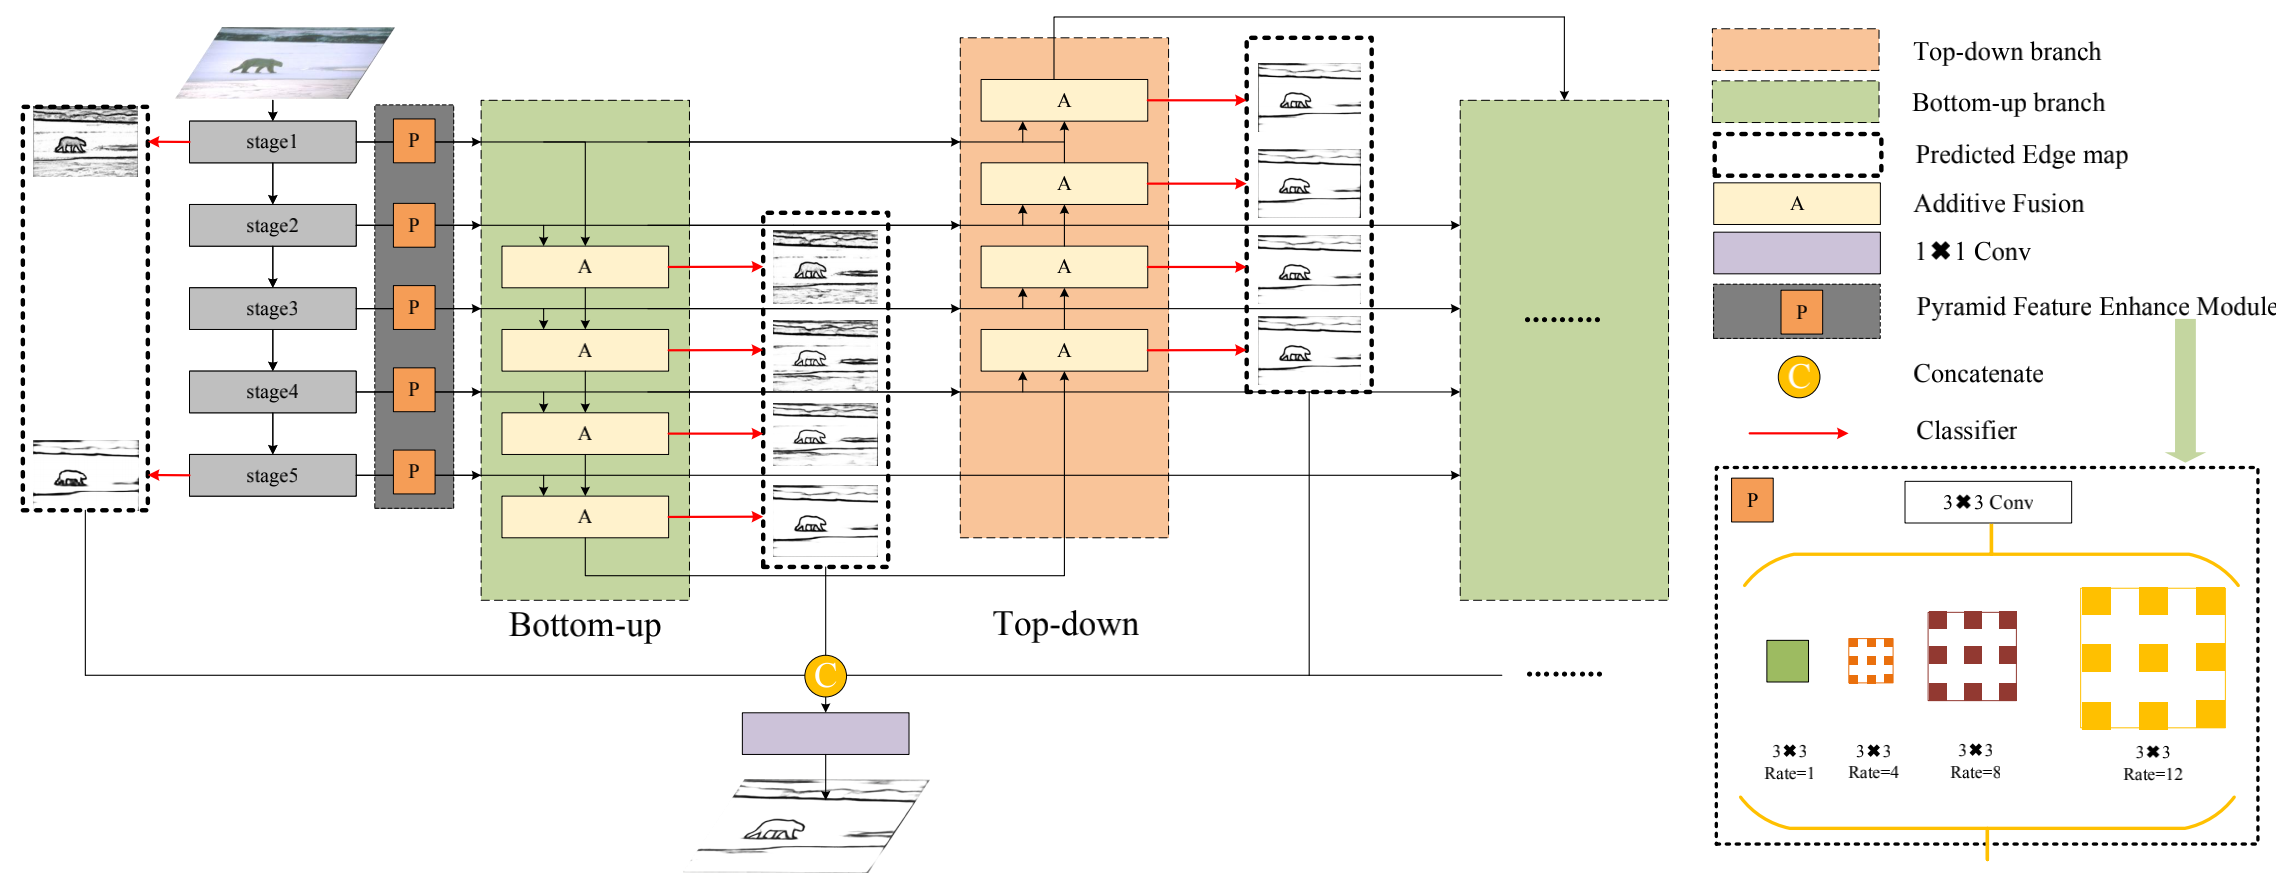
\includegraphics[width=1.0\textwidth]{framework.png}
    \caption{网络的基于架构图。输入是任意尺寸的图片,网络的输出是具有和输入同样大小的边缘概率图。特征提取网络使用的是常见的VGG16网络设计}
    \label{framework2}
\end{figure}

\subsection{金字塔特征提取网络}
金字塔特征提取网络用于提取具有丰富上下文信息的多层次特征,具体来说改部门可以区分为两个小部分:特征提取网络和特征金字塔结构。我们使用$V$代表基本的特征提取器,特征提取网络中包含大量的卷积层、池化层和激活函数层。在具体实现中,我们使用VGG16网络作为我们的特征提取网络。给定一个输入图片$I$,基本的特征提取网络能够在每个VGG网络的阶段生成对应的边缘特征$F_i\in \mathbb{R}^{h^i \times w^i \times C}(i=1,2,...,L)$ 。在得到边缘特征$F_i$之后,我们利用一个$3 \times 3 \times  32$的卷积层用于特征降维,将所有$F_i$特征的通道数都降低到32,从而在后续的侧枝计算中大大减小了对应的计算量。在之后的表述中,我们使用$L$代表基本特征提取网络中的阶段数,其中$i$代表第$i$个阶段。

在获得了经过特征降维之后的特征图$F_i\in \mathbb{R}^{h^i \times w^i \times C}$之后,我们使用了一系列膨胀卷积组成一个金字塔结构,从而获取了能够覆盖多个不同大小感受野的边缘特征。我们使用${A_r \in \mathbb{R}^{3 \times 3 \times C}}(r=r_1,r_2,...,r_K)$来表示这些卷积层的卷积核,而其中$C$代表卷积核的个数即输出的通道数,$r$
代表了膨胀卷积的采样率,$K$代表了带孔卷积的个数。注意到分辨率是在边缘检测这样一个图像理解任务中非常重要的因素,我们利用双线性插值对特征图进行了上采样,将所有的特征上采样到了输入图片的大小,方便后续的特征结合。在这里我们同样尝试了反卷积、像素随机化等上采样技术,但是上述的上采样方法并没有取得良好的效果,反而因为相关计算量的上升导致网络容易陷入过拟合的陷阱中,造成效果的下降。

我们可以将特征金字塔的操作定义为下面的式子:
\begin{equation}
    P_i = U(\sum\nolimits_{r=r_1}^{r_k}(A_r \ast F_i) + F_i)
\end{equation}

其中$\ast$代表膨胀卷积操作,$P_i$代表生成特征图,$U$代表上采样模块,这里使用的是双线性插值网络。 除此之外,我们为了保证梯度的回传,我们在$P_i$和$F_i$之间添加了残差的连接。

而对应的特征金字塔结构,我们使用了采样率为1、4、8和12的膨胀卷积并联构成,构成一个金字塔结构。之后同一个一个简单的逐元素相加得到特征金字塔结构的输出。


\subsection{自底向上和自顶向下的特征结合}

给定输入图片$I$,我们能够通过上面介绍的金字塔特征提取网络得到覆盖多个感受野信息的边缘特征$P_i \in \mathbb{R}^{H \times W \times C}$。我们在这部分将会介绍自底向上和自顶向下的特征结合部分,我们利用连续的自底向上和自顶向下的特征结合网络去优化生成的圆边特征$P_i$。其中通道注意力机制引导的特征合成模块在自底向上和自顶向下的特征结合网络中扮演特征结合的部分,具体的这个部分将在下一章介绍,对应式子中这一部分我们将用$AAM$代替。

\textbf{自底向上的网络架构。} 给定一系列特征金字塔模块生成的特征$P_i$,一个自底向上的网络架构能够让较低层的特征逐渐建和高层正紧,进而生成对应结合后的特征$BU_i\in \mathbb{R}^{H \times W \times C}(i=1,2,..,L-1)$.。对于一个较低层的特征$P_{i-1}$和较高层的特征$P_i$,我们能够生成对应结构后的特征通过公式\eqref{eq:bottom_up}。
\begin{equation}
    BU_i =
    \begin{cases}
    AAM(P_{i+1}, P_{i}), &\text{if $i = 1$} \\
    AAM(P_{i+1}, BU_{i-1}), &\text{if $i = 2,3,...,L-1$}
    \end{cases}
    \label{eq:bottom_up}
 \end{equation}
通过自底向上网络结构的运算方式,我们能够发现该架构下最终一层的特征图相比之前的特征图能够携带更加丰富和准确的信息,这一观现象在也在图\ref{visual_side_out}上做了可视化的验证。在后续的实验中,我们也能通过定量的分析来证明我们的结论和自底向上网络架构的作用。

\textbf{自顶向下的网络架构。} 给定一系列特征金字塔模块生成的特征$P_i$,一个自顶向下的架构能够将最高层的特征逐渐向低层传递 ,和低层特征图进行结合,从而得到准确的边缘预测结果。队医一个较高层的特征$P_i$和一个较低层的特征$P_{i-1}$,一个自顶向下的结构能够生成对应的特征图$TD_i\in \mathbb{R}^{H \times W \times C}(i=L-1,L-2,...,1)$通过公式\eqref{eq:top_down}
\begin{equation}
    TD_i \!\!=\!\!
    \begin{cases}
     {AAM}(P_i, P_{i+1}), \! &\text{if $i = L-1$}\\
     {AAM}(P_i, TD_{i+1}),\! &\text{if $i = L\!-\!2, L\!-\!3,...,1$}
    \end{cases} 
    \label{eq:top_down}
\end{equation}

在定义了单向的特征传递架构自底向上和自顶向下架构之后,我们可以将两种单向的架构结合在一起,下面我们将介绍我们提出的结合自底向上和自顶向下的双向架构。通过这样的双向架构,我们能够充分利用单向网络的优势并且弥补单向网络的特征遗忘问题,达到互补的效果。

\textbf{结合自底向上和自顶向下的双向架构。}在 这部分,我们将介绍结合结合自底向上和自顶向下的双向架构。按照这样的网络推理机制,$TD_{i}^{n}$代表在自顶向下架构中位于第$i$层,位于第$n$个特征融合架构上得到的特征。按照同样的规则,我们分别定义第$i$层从自底向上架构中和自顶向下的结构中得到的特征为$BU_{i}^{n}$, $TD_{i}^{n} (n=1,2,...,N, i=1,2,...,L-1)$。总共的自底向上和自顶向下的个数定义为$N$。对应的自底向上架构上的网络输出可以定义为公式\eqref{eq:bottom_up_multi}。
\begin{equation}
    BU_i^n \!\!=\!\!
    \begin{cases}
    AAM(P_{i+1}, TD_1^{n-1}),\!\! &\text{if $i = 1$ and $n \geq 2$} \\
    AAM(P_{i+1}, P_{i}),\!\! &\text{if $i = 1$ and $n = 1$} \\
    AAM(P_{i+1}, BU_{i-1}^{n}),\!\! &\text{if $i = 2,3,...,L-1$}
    \end{cases}
    \label{eq:bottom_up_multi}
 \end{equation}

而对应自顶向下架构中生成的特征定义为公式\eqref{eq:top_down_multi}:
\begin{equation}
    TD_i^n \!=\!\!
    \begin{cases}
     {AAM}(P_i, BU_{L-1}^{n-1}),\!  &\text{if $i\! = \!L\!-\!1$ and $n \geq 2$}\\
     {AAM}(P_i, P_{i+1}), \! &\text{if $i \!=\! L\!-\!1$ and $n = 1$}\\
     {AAM}(P_i, TD_{i+1}^{n}), \!&\text{if $i \!=\! L\!-\!2, L\!-\!3,...,1$}
    \end{cases}
    \label{eq:top_down_multi}
\end{equation}
 
\subsection{注意力机制引导的特征结合模块}

在通过引入上述的连续的自底向上和自顶向下的双向架构之后,我们能够充分利用多层次的特征用于生成图像边缘特征图。在这部分,我们将介绍在上述的自底向上和自顶向下的双向架构中的AAM,即注意力机制引导的特征结合模块,具体的网络架构图如图\ref{aam}所示。这部分的特征结合模块上一章节的特征结合模块在设计放慢有几处不同:(1)在这一章的方法中我们使用了通道注意力机制,而上一章中我们使用的空间注意力机制用于引导合成;(2)在这里我们移除了上述的残差块用于减小网络的计算量。 (3)在通道注意力机制中我们使用了多分支的注意力机制用于提高通道注意力机制的效果。

针对第一点改动,我们在本章中尝试过使用空间注意力机制、通道注意力机制和空间通道注意力机制结合的三种模式,经过的实际的实验效果我们发现通道注意力机制相比空间注意力机制能够取得更好的效果;而空间通道注意力机制结合的模式相比单独的空间注意力机制并没有效果的提升,所以最后我们采用的通道注意力机制。分析其中的原因,可能是因为边缘检测中对应的边缘点在图中的像素个数过少,对应的空间注意力机制相比通道注意力机制自动化地学习更为困难。 针对第二点改动,我们对侧枝网络中的残差块进行分析,可以发现残差块在输入特征图较大的情况下需要很大的计算消耗,但是对于最后的结果帮助并不大。考虑到模型最后的计算速度和计算开销,我们去除了相应的残差块设计,采用了最简单的逐元素相加的策略。针对第三点改动,我们在尝试仿照金字塔结构在注意力机制中加入多分支提高最后的效果。
\begin{figure}[h!]
    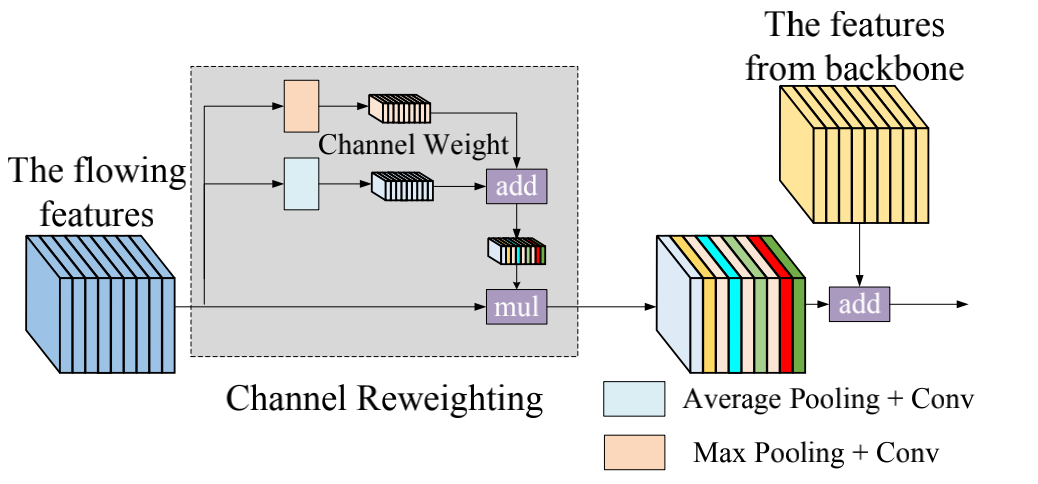
\includegraphics[width=1.0\textwidth]{aam.png}
    \caption{注意力机制引导的特征结合模块具体结构图}
    \label{aam}
\end{figure}

在这一小节中,定义$f\in \mathbb{R}^{H \times W \times C}$为任意尺寸的从其他层传输而来的特征,对应的通道数$C$。首先使用对$f$使用全局池化层获得对应的向量$v \in \mathbb{R}^{C}$,其中包含了$f$中每个通道的全局信息。之后利用两个连续的1$ \times$ 1卷积层用于挖掘向量$v \in \mathbb{R}^{C}$中每个通道的重要性和每个通道之间的关系。这里的1$ \times$ 1卷积层作用和全连接层一样。之后通过一个Sigmoid的激活函数层将对应的通道权重归一化到$[0,1]$之间。整个操作可以定义为公式\eqref{eq:channel_att}。
\begin{equation}
    w = Sigmoid(Conv(\sigma (Conv(Pool(f)))))
    \label{eq:channel_att}
\end{equation}

其中$w$定义为通道权重,$\sigma$定义为对应的ReLU损失函数,$Conv$定义为卷积层而$Pool$代表池化层。所以注意力机制引导的特征结合模块引导的AAM可以定义为公式\eqref{eq:aam}。
\begin{equation}
    AAM(P_{i}, f) = w * f + P_{i}
    \label{eq:aam}
\end{equation}

而在通道注意力机制中,我们借鉴了金字塔结构的作用,同样收到\citing{DeepEdge}的启示,我们引入了两种不同的池化层结构构成两个支路,最后的通道注意力机制的通道权重是两个支路的相加结果。这样的多支路注意力机制设立也能少许提高网络的效果。


\section{双向网络的优化部分}
传统的交叉熵函数并不能满足正负样本不平衡的边缘检测任务的要求。我们在这里沿用之前方法中的带权重的二分类交叉熵网络,网络同样定义如下:
\begin{equation}
\begin{aligned}
L_{ce}(W) = -\gamma \cdot \beta \sum\nolimits_{g_{i} \in G_{+}}\log P(g_{i} = 1 | I ; W) \\
- (1 - \beta) \sum\nolimits_{g_{i}\in G_{-}}\log P(g_{i} = 0 | I ; W)
\end{aligned}
\end{equation}
具体的参数表达式和第三章中叙述的表达式相同,观察到网络产生的边缘比较粗宽,所以在最后的结果在评测之后需要进行非极大值抑制的操作让边缘变细。于是我们尝试对于网络预测边缘粗宽的问题的问题进行解决。

在针对训练网络时正负样本不均衡的问题进行调研时,除了像上述一样对正负样本引入不同的权重进行调节之外,在医学图像分割领域,面对正负样本不均衡问题时,常常引入Dice损失函数。

Dice函数的定义来自Dice系数,是一种定义两个集合相似度的一种度量方式,其中Dice系数的取值范围在$[0,1]$之间。而引入计算机视觉领域,我们可以将网络产生的预测结果和对应的标注真值都看作两个由像素点构成的集合。相比比交叉熵函数对于逐像素点进行损失函数计算最后在汇总在一起(pixel leve),Dice更像是一个在输入图片全局上进行的损失函数度(image-level)。在我们的网络中Dice损失函数的定义如式所示。
\begin{equation}
    L_{d}(W) = \frac{\sum_{i}^{N}e_{i}^{2} + \sum_{i}^{N}g_{i}^{2}}{2\sum_{i}^{N}e_{i}g_{i}}
    \label{equ:dice_loss}
\end{equation}
其中$e_{i}$代表网络预测边缘图中的一个像素,而$g_i$代表标注真值中的一个像素。通过Dice损失函数能够显著让网络预测边缘变细,但是仍然不能代替非极大值抑制的效果,这方面的研究也可以作为一个未来的改进方向。

\textbf{Dice损失函数的分析。}为了分析Dice Loss的引入原因和它对网络预测边缘的效果。首先从之前常用的交叉墒损失函数入手,常规的交叉墒函数作为边缘检测的训练损失,对于不平衡的数据样本分布,网络训练学习非常困难。尽管对交叉墒损失函数添加了正负样本平衡的因子,也很难完全解决交叉墒函数的固有问题。因为交叉墒函数的损失是对每一个像素,计算一个图片上像素损失的平均值。而对于像素级别的计算,每个像素的计算都是独立的,无法知道是否其领域像素也为边缘像素,即缺乏一个全局的损失估计。这样的性质使得交叉墒损失无法考虑到全局信息,对于一个图片级别的预测是不足的(image-level)。

Dice损失函数的表达如式\ref{equ:dice_loss}所示。在边缘检测中,公式中的$e_{i}$和$g_i$的像素值都为0或1,代表该像素是否为边缘点。因此Dice损失函数实际表达了样本真值的所有像素点和预测结果的所有像素点,两个点集合的一个相关系数。而在训练过程中,要使得Dice损失函数变小,则需要使得损失函数的分母$\sum_{i}^{N}e_{i}g_{i}$增大,同时尽可能减小损失函数的分子$\sum_{i}^{N}e_{i}^{2} + \sum_{i}^{N}g_{i}^{2}$。分母的增大即使得网络预测的真值数量和样本真值的像素点交集越来越大,而分子的减小,对于边缘检测来说,则是要尽可能减少预测样本中的边缘点个数($e_{i}==1$)。

总的来说,网络对Dice损失函数的优化使得预测结果和样本真值的像素点集交集越来越大,同时网络对于预测样本边缘点个数也越来越少,更少的预测边缘点个数也促使Dice损失函数能够极大的让网络的预测边缘变细。并且Dice损失函数能够让网络从全局的角度进行优化,也进一步能提高边缘预测的准确度。

网络最终的损失函数定义如公式\eqref{eq:loss}。其中表示为交叉熵函数和Dice损失函数的加权融合结构。其中$\lambda_d$代表Dice损失函数的权重,用于平衡Dice损失函数和带权重的交叉熵损失函数。
\begin{equation}
    L(W) = L_{ce}(W) + \lambda_{d} L_{d}(W)
\label{eq:loss}
\end{equation}

为了获取最终结果,我们首先根据所有自底向上和自顶向下双向结构中的侧枝网络输出$E_{i}^{n} (i=1,2,...,L; n=1,2,...,N)$经过类似HED中的线性加权得到融合后的结果$E_{fuse}$。其中$E_{i}^{n}$代表通道注意力引导的特征融合模块的结果经过一个 $1 \times 1 \times 1$卷积之后得到的特征图。在HED工作的引导下,我们将生成的融合结果$E_{fuse}$和侧枝输出$E_{i}^{n}$的平均结果作为最终的输出。 

在网络训练策略上,我们同样沿用了之前工作常用的深度监督策略,这样的策略有注意避免梯度消失问题,并且能够在每个侧枝输出上保证一个个较为准确的边缘图,有助于生成最终的结果。

在实际实现中,我们采用了Pytorch深度学习框架\citing{Pytorch}。我们使用了带动量的梯度下降(SGD)作为网络的优化算法,其中学习率设置为$1e-7$,动量参数设置为$2e-4$, 一个批次的大小(batch size)设置为10。我们在BSDS500数据集上训练了15000次,而在NYUDv2数据集上训练了30000次。

\section{实验设计部分}
在这部分我们将主要介绍相关的消融实验和对比实验,所使用的数据集和评测指标等实验基础设置。从实验中我们能够定量分析每个模块的作用,并且体现我们方法的优越性。
\subsection{数据集介绍}
本文这部分和上一章方法一样同样采用了BSDS500和NYUDv2数据集,详细的具体介绍可以参照2.5.1章节。

\subsection{评测指标介绍}

这一章的评测指标仍然采用边缘检测通用的指标全数据集最优尺度(ODS)、图片最优尺度(OIS)和平均准确率(AP)。其中在评测指标之前,我们仍然需要使用非极大值抑制的方法对输出的边缘图片进行变细处理。在评测过程的匹配阶段,我们对BSDS500的匹配阈值设置为0.0075,对NYUDv2的匹配阈值设置0.011。指标的具体含义可以参照2.5.2章节的介绍。

\subsection{数据增强处理}

对于BSDS500数据集,我们仍然采用了和章节3.5.3同样的数据增强策略、:对于每一张图片,我们分别将其缩放为原来的0.5倍和1.5倍我们对每种数据尺寸下的每张图片从0度到337.5度进行了16个角度(22.5, 45, 67.5, 90, ...,337.5)的旋转,并且裁切旋转后的最大内接矩形为最后的旋转图片,除此之外,我们还对每种数据尺寸下、每个旋转角度下的图片进行水平方向的翻转,最终扩张为原训练集尺寸的96倍,最后达到了28800张训练集图片。

对于NYUDv2数据集来说,我们同样也做了大量数据增强以满足深度神经网络的训练需求:我们对同样也将其缩放为原来的0.5倍和1.5倍、将图片旋转为90,180,270三个角度,并且对每种角度下的图片都做了水平翻转,最终达到18096张训练集合图片。

\subsection{网络消融实验}
本节我们将对网络的结构和相关设计采用消融实验的方法证明其有效性,通过消融实验我们可以观察到不同网络设计下网络的效果,更好的理解我们提出的最终结构。在本节的描述中,基线方法(Baseline)代表类似HED的结构:每个阶段独立处理边缘特征,最后通过一个拼接和$1 \times 1 \times 1$卷积的形式将不同输出的边缘图进行线性加权得到最终的边缘图结果。

\textbf{不同的网络变体结构。} 我们首先探索了网络不同变体结构的效果。在这里我们主要讨论两个类似的变体,主要是架构的顺序问题:1)先采用自底向上,衔接自顶向下网络 2)先采用自顶向下,衔接自底向上网络。我们称为1)中的变体为"v1",2)中的变体为"v2"。我们对两种变体作为相关效果的评测,并且选择了变体"v1"作为最终的结构。从表格\ref{tab:variants}中,我们能够观察到"v1"和"v2"变体的效果都会比基线方法的效果号,这也说明了在不同层之间进行信息传递的重要性和必要性。
\begin{table}[h!]
    \caption{不同变体架构之间的效果对比}
    \centering
    \scalebox{1.0}{\begin{tabular}{p{2cm}|p{1.5cm}p{1.5cm}p{1.5cm}}
    \hline
    变体结构  & ODS & OIS & AP \\
    \hline
    \hline
    基线方法 & 0.794  & 0.812 & 0.779     \\
    \hline
    n=1(v1)       & 0.800  & 0.818 &  0.809     \\
    n=2(v1)       & \textbf{0.810}  & \textbf{0.827} & 0.862      \\
    n=3(v1)       & 0.806 & 0.824 &   0.847  \\
    \hline
    n=1(v2)       & 0.801  & 0.819 & 0.830      \\
    n=2(v2)       & 0.808  & 0.825 & 0.864     \\
    n=3(v2)       & 0.805  & 0.822 & 0.839     \\
    \hline
    \end{tabular}}
    \label{tab:variants}
\end{table}

\textbf{不同的自底向上和自顶向下的架构个数。} 从表格\ref{tab:variants}中,我们可以观察到在一定的架构数目下,双向的自底向上和自顶向下的设计能够显著提高边缘检测的效果。但是当架构数目过多的情况下,对应的表现会轻微下降。分析其中的原因,可能是因为过于复杂和深度的网络使得网络变得更加困难,而且参数量增大之后可能会造成训练的过拟合现象,这也是表现轻微下降的一个可能原因。尽管如此,我们能发现我们提出的双向的架构相比基线方法和单向方法,能够取得更好的效果。

\textbf{边缘图层次(Prediction-level) vs. 特征层次(Feature-level)。}我们的方法相比于之前的BDCN方法的一个区别是我们的方法采用了特征层次的信息传递而不是边缘图层次的传递。因为我们认为特征图相比边缘图包含耿耿福的特征信息。在表格\ref{tab:method}中,我们同样比较边缘图层次和特征层次的信息流传递方式的效果。从表\ref{tab:method}中,我们可以作出如下的结论:1)边缘图层次的传递对于边缘检测来说是有帮助的,它能够在ODS、OIS和AP上分别提高0.3\%、0.3\%、5.8\%。 (2)特征层次的信息传递显著提高了边缘检测网络的效果。相比于基线方法,特征层次的信息流在ODS、OIS和AP上分别提高了1.1\%、0.9\%和6.1\%,相比于边缘图层次的信息流传递能够取得更好的效果。上述的实验结果也证明了特征层次的信息流传递机制和双向的基于自底向上和自顶向下的网络结构能显著提高边缘检测的效果。
\begin{table}
    \centering
    \caption{不同的信息传递机制和注意力机制引导的特征融合网络的消融实验效果}
    \scalebox{1.0}{
    \begin{tabular}{p{3cm}|p{1.5cm}p{1.5cm}p{1.5cm}}
    \hline
    方法  & ODS & OIS & AP \\
    \hline
    \hline
    Baseline & 0.794  & 0.812 & 0.779     \\
    \hline
    Prediction-level       & 0.797  & 0.815 & 0.837     \\
    Feature-level        & 0.805  & 0.821 & 0.840      \\
    \hline
    AAM(average)       & 0.809  & 0.826 & 0.848    \\
    AAM(max)       & 0.809  & 0.825 & 0.840     \\
    AAM(two-stream)   & \textbf{0.810}  & \textbf{0.827} & \textbf{0.862}     \\
    \hline
    \end{tabular}
}

\label{tab:method}
\end{table}

\textbf{注意力机制引导的特征融合模块。}在表\ref{tab:method}中,我们同时也讨论了通道注意力引导的特征融合模块和不同的池化层策略对最后结果的影响。"Feature-level"代表不使用通道注意力机制引导合成的特征结合模块。通过表\ref{tab:method}的实验我们可以发现,特征结合模块中的通道注意力机制通过过滤特征中错误和冗余的信息、强化重要信息进而达到了提高边缘检测效果的作用。而利用两种不同的池化层机制能够略微提高最后的表现能力。分析其中的原因,可能是因为不同的池化层机制能够在通道权重中捕捉不同的全局信息,这会促使整个通道注意力机制更加鲁棒和有效。


\textbf{侧枝网络的输出。}我们将探究在我们双向特征传递网络的架构中不同侧枝网络的输出对结果的影响。从表格\ref{tab:stages}中,我们可以发现在我们的网络中的侧枝输出能够逐渐产生更好的效果,而通过所有侧枝网络输出得到的最终结果能够取得最好的性能。相比于基线方法,我们的方法同时在每个侧枝输出上都能够取得更好的效果,证明了双向特征优化的网络中特征图的流动对于整个网络性能有着积极的影响。


从表格\ref{tab:stages}中,我们可以发现在我们的网络中的侧枝输出能够逐渐产生更好的效果,而通过所有侧枝网络输出得到的最终结果能够取得最好的性能。相比于基线方法,我们的方法同时在每个侧枝输出上都能够取得更好的效果,证明了双向特征优化的网络中特征图的流动对于整个网络性能有着积极的影响。
 

\textbf{参数敏感度的分析。}我们将探究在我们双向特征传递网络的架构中不同网络参数的输出对结果的影响。在表格\ref{tab:channel}中,我们分析了特征提取的金字塔网络中,不同的特征维度的输入对于整体网络的影响。从结果中可以发现32维度的特征能够取得最好的效果,且网络对于不同特征维度参数的选取具有一定的鲁棒性,不会因为参数的变动造成巨大的效果变化。对于特征维度较小的情况,可能不具有充分的特征表达能力,影响了最后效果的表达。而大的特征维度对于边缘检测问题可能造成参数冗余,训练过拟合的问题。
\begin{table}
    \centering
    \caption{网络特征提取的金字塔架构中特征的维度对于最后效果的影响}
    \scalebox{1.0}{
    \begin{tabular}{p{3cm}|p{1.5cm}p{1.5cm}p{1.5cm}}
    \hline
    特征维度  & ODS & OIS & AP \\
    \hline
    \hline
    16 & 0.807  & 0.821 & 0.846     \\
    24       & 0.809  & 0.825 & 0.852     \\
    32       & \textbf{0.810}  & \textbf{0.827} & \textbf{0.862}     \\
    64        & 0.810  & 0.825 & 0.860      \\
    128       & 0.808  & 0.826 & 0.851    \\
    \hline
    \end{tabular}
}
\label{tab:channel}
\end{table}

同时对于特征金字塔中的分支个数,我们在表\ref{tab:K}中进行了参数效果的分析。对于分支数量为1的结果,代表只有一个分支,即为单尺寸的结构,不包含金字塔结构。从实验\ref{tab:K}中可以发现金字塔结构提取的多尺度信息对于最终结果有较大的帮助,同时我们测试得到三个并行分支数量能够得到更好的结果。后续分支数量的增加,并不会带来效果的提升。
\begin{table}
    \centering
    \caption{网络特征提取的金字塔架构中金字塔分支数对于最后效果的影响}
    \scalebox{1.0}{
    \begin{tabular}{p{3cm}|p{1.5cm}p{1.5cm}p{1.5cm}}
    \hline
    分支数量  & ODS & OIS & AP \\
    \hline
    \hline
    1 & 0.805  & 0.822 & 0.833     \\
    2       & 0.807  & 0.826 & 0.852     \\
    3       & \textbf{0.810}  & \textbf{0.827} & 0.862     \\
    4        & 0.809  & 0.826 & \textbf{0.864}     \\
    \hline
    \end{tabular}
}
\label{tab:K}
\end{table}


\begin{table}
    \centering
    \caption{基线方法和我们的方法在侧枝网络输出结果上的表现}
    \newcommand\tikzmark[1]{\tikz[remember picture] \node (#1) {};}
    \begin{tabular}{|c|l|l|l|}
    \hline
    \multirow{2}*{侧枝输出} & \multicolumn{3}{c|}{ODS}\\
    \cline {2-4}
     & 基线方法 & T=1 &T=2 \\
    \hline
    \hline
    stage1 & 0.722  & \color{gray}{0.743}  & 0.804 \tikzmark{d}     \\
    stage2       & 0.749    & 0.770 \tikzmark{a} & 0.803    \\
    stage3       & 0.771       & 0.788 & 0.803   \\
    stage4 & 0.756     & 0.802  & 0.804 \tikzmark{c}    \\
    stage5 & 0.757   & 0.803\tikzmark{b}  & \color{gray}{-}       \\
    \hline
    fuse & 0.794  & \multicolumn{2}{|c|}{\textbf{0.810}}  \\
    \hline
    \end{tabular}
    \tikz[remember picture,overlay] \draw[->] (a.center -| b.center) -- (b.center);
    \tikz[remember picture,overlay] \draw[->] (c.center -| d.center) -- (d.center);
    \label{tab:stages}
\end{table}


\textbf{上采样模块的选择。}我们同时对比了不同的上采样模块对网络最终结果的影响。我们尝试了使用三种不同的上采样策略,从中寻找一种最合适的上采样策略:双线性插值、反卷积和像素随机化。其中像素随机化被广泛应用在了超分辨率领域。从表格\ref{tab:upsample}中我们可以发现像素随机化没有取得令人满意的结果,而带有学习参数的反卷积在网络中并没有取得明显的效果提升。我们分析出现这种现象的原因:固定参数的双线性插值和后续的卷积层已经能够起到了和反卷积相同的作用。而带有学习参数的反卷积会提高网络的参数量,导致网络相比之前更加难以训练。同样的现象也发生在文章\citing{Crisp}中。在这篇文章中,作者使用了组合卷积(grouped)卷积和组合(grouped)反卷积去降低网络的复杂度,对于边缘检测来说更加稳定。
\begin{table}
    \centering
    \caption{不同上采样模块的对比实验效果}
    \small
    \begin{tabular}{l|lll}
    \hline
    上采样模块  & ODS & OIS & AP \\
    \hline
    \hline
    我们的方法(pixel shuffle)      & 0.797  & 0.814 & 0.808     \\
    我们的方法(deconv)       & 0.810  & 0.826 & 0.862      \\
    我们的方法(bilinear interpolate)    & 0.810  & 0.827 & 0.862     \\
    
    \hline
    \end{tabular}
    \label{tab:upsample}
    \end{table}}

\textbf{损失函数和训练策略。}我们的模型通过一个由交叉熵和Dice损失函数构成的损失函数进行训练,并且通过深度监督的训练策略进行训练。表格展示了深度监督在边缘检测中的作用。同时从表格\ref{tab:loss}中,我们可以发现加入Dice损失函数之后,网络边缘检测的效果仅有着微小的提升,这可能是因为边缘的细化效果会被非极大值抑制覆盖。从后面的可视化结果,如图\ref{fig:loss}所示,我们可以发现Dice损失函数对于细化边缘的作用,细化的边缘对于后续的光流预测和目标候选生成都有着很大帮助。
\begin{table}
    \centering
    \caption{表格为训练策略和损失函数的消融实验}
    %\small
    \begin{tabular}{l|lll}
    \hline
    训练策略 & ODS & OIS & AP \\
    \hline
    \hline
    network(w/o deep supervision) & 0.796  & 0.814 & 0.784     \\
    network(only dice loss) & 0.790  & 0.807 & 0.827     \\
    network(w/o dice loss)     & 0.809  & 0.827 & 0.860     \\
    network(w/ dice loss)       & 0.810  & 0.827 & 0.862      \\
    \hline
    \end{tabular}
    \label{tab:loss}
\end{table}


\begin{figure}[h!]
    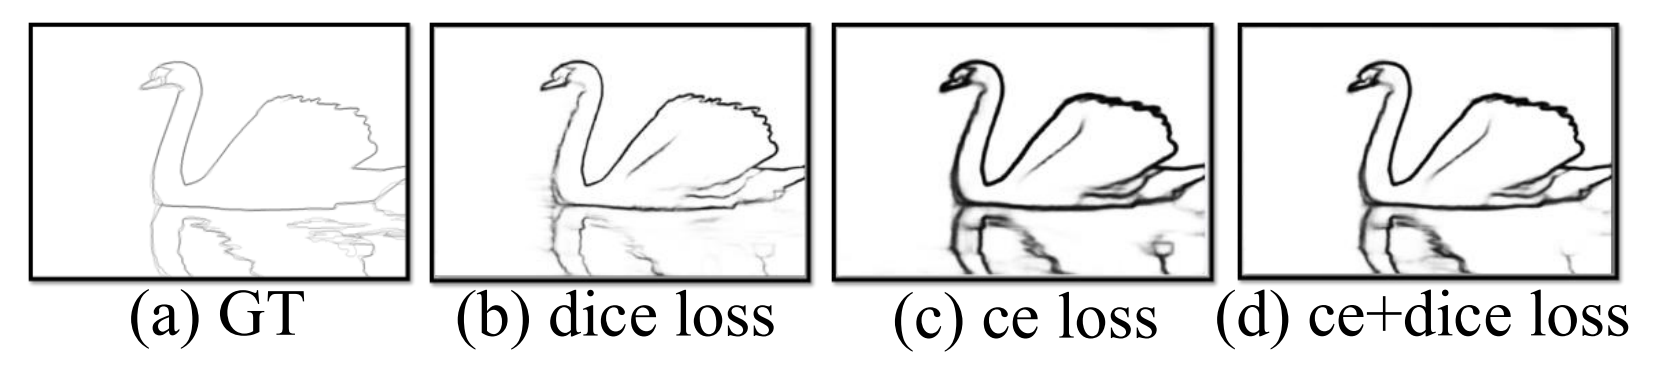
\includegraphics[width=1.0\textwidth]{loss_visual.png}
    \caption{不同损失函数对网络最终结果的影响。可以发现Dice Loss对边缘细化有着跟好的效果。(a)标注真值;(b)只用Dice损失函数训练的结果;(c)交叉熵损失函数训练的结果;(d)采用交叉熵和Dice损失函数综合训练之后的结果}
    \label{fig:loss}
\end{figure}

\begin{table}[h!]
    \begin{center}
        \caption{网络的计算资源和运行时间复杂度分析, 对应的时间复杂度在Ubuntu 16.04, CUDA 9和Nvidia 1080Ti单卡上进行测试}
        \label{tab:cost2}
        \begin{tabular}{c|c|c}
            \toprule % <-- Toprule here
            \textbf{主干网络FLOPs} & \textbf{全部网络FLOPs} & \textbf{FPS}\\
            \midrule % <-- Midrule here
            16.11G&20.26G&25\\    
            \bottomrule % <-- Bottomrule here
        \end{tabular}
    \end{center}
\end{table}

\subsection{和其他方法的对比}
我们在两个公开数据集BSDS500和NYUDv2上对网络的表现和其他方法进行横向的对比。通过在两大数据集上的对比我们可以发现我们的方法在两大数据集上都取得了最好的结果。
\begin{table}[h!]
    \centering
    \caption{在BSDS500数据集上和其他方法的对比结果}
    \scalebox{1.0}{%
        \begin{tabular}{l||lll}
            \hline
            方法 & ODS & OIS & AP \\
            \hline
            \hline
            Human     & 0.803  & 0.803 & -     \\
            \hline
            Canny\citing{Canny}     & 0.611  & 0.67 & 0.520     \\
            Pb\citing{Pb}       & 0.672  & 0.695 & 0.652      \\
            MCG\citing{traditional_5}       & 0.744  &   0.777 &   0.760     \\
            OEF\citing{OEF}       & 0.746  &   0.770 &  0.815      \\
            \hline
            DeepEdge\citing{DeepEdge}       & 0.753  &  0.772 &  0.807      \\
            DeepContour\citing{DeepContour}       &  0.757  &  0.776 &  0.790      \\
            HED\citing{HED}       & 0.788   &  0.808 &  0.840     \\
            COB\citing{COB}       &  0.793  &  0.819 &  0.849      \\
            RCF\citing{RCF}       &  0.798  &  0.815 &  -      \\
            LPCB\citing{Crisp}       & 0.800  & 0.816 &  -      \\
            CED\citing{CED}       &  0.794  &  0.811 &  0.847      \\
% 			CED-MS       &  0.803  &  0.820 &  0.871      \\
            BDCN\citing{BDCN}       &  0.806  &  0.826 &  0.847      \\
            \hline
            \color{gray}{AMH-Net(ResNet50)\citing{AMHNet}}    &  \color{gray}{0.798}  &  \color{gray}{0.829} &  \color{gray}{0.869}      \\
            \color{gray}{CNet(ResNet101)\citing{CNet}}    &  \color{gray}{0.805}  &  \color{gray}{0.819} &  \color{gray}{0.851} \\
            \hline
            BAN    &  \textbf{0.810}  &  \textbf{0.827} &  \textbf{0.862}      \\
            BAN-MS    &  \textbf{0.816}  &  \textbf{0.834} &  \textbf{0.870}      \\
            \hline
        \end{tabular}
    }
    \label{tab:bsds_sota}
\end{table}

表格中\ref{tab:loss}中,我们在BSDS500数据集上对比了我们的方法和其他方法的效果。从表格\ref{tab:loss}中我们发现我们的方法在单张图片输入的情况下在ODS的F值上达到了0.810,而对于多尺度图片输入我们的网络能够取得了0.816的效果,超过了其他的方法。其中在BSDS500上我们的方法 能够超过一些方法在多尺度输入下的效果(CED-MS),和一些利用残差网络为主干网络的方法例如AMH-Net和CNet。

\begin{table}[h!]
	\centering
    \caption{在NYUDv2数据集上和其他方法的对比结果}
	\scalebox{1.0}{\begin{tabular}{l||lll}
		\hline
		方法 & ODS & OIS & AP \\
		\hline
		gPb-UCM     & 0.631  & 0.661 & 0.562     \\
		OEF    & 0.651  &  0.667 & 0.653      \\
		gPb+NG     & 0.687  & 0.716 & 0.629     \\
		SE     & 0.695  & 0.708 &  0.719      \\
		SE+NG+       &   0.706  & 0.734 &  0.549      \\
		\hline
		HED-RGB       &  0.720  & 0.734 & 0.734      \\
		HED-HHA       & 0.682  & 0.695 & 0.702      \\
		HED-RGB-HHA       & 0.746  &   0.761 &   0.786     \\
		\hline
		RCF-RGB       & 0.729  &   0.742 &  -      \\
		RCF-HHA       & 0.705  &  0.715 &  -      \\
		RCF-RGB-HHA       &  0.757  &  0.771 &  -      \\
		\hline
		LPCB-RGB       & 0.739   &  0.754 &  -     \\
		LPCB-HHA       &  0.707  &  0.719 &  -      \\
		LPCB-RGB-HHA       &  0.762  &  0.778 &  -      \\
		\hline
		BDCN-RGB       & 0.748  & 0.763 &  0.770      \\
		BDCN-HHA       &  0.707  &  0.719 &  0.731      \\
		BDCN-RGB-HHA       &  0.765  &  0.781 &  0.813      \\
		\hline
		\color{gray}{AMH-Net(ResNet50)-RGB-HHA} & \color{gray}{0.771} & \color{gray}{0.786} & \color{gray}{0.802} \\
		\color{gray}{CNet(ResNet101)-RGB-HHA} & \color{gray}{0.762} & \color{gray}{0.781} & \color{gray}{0.797} \\
		\hline
		BAN-RGB       &  \textbf{0.755}  &  \textbf{0.770} &  0.760      \\
		BAN-HHA       &  0.707  &  0.718 &   0.710    \\
		BAN-RGB-HHA    &  \textbf{0.773}  & \textbf{0.786} &  0.790    \\
		\hline
	\end{tabular}}
	\label{tab:nyud_sota}
\end{table}

在表格\ref{tab:nyud_sota}中,我们对比了我们的方法在NYUDv2上和其他方法的对比效果图。在NYUDv2上最终的输出是 NYUDv2数据集中RGB图片和HHA图片得到的预测结果的平均值。从表格\ref{tab:nyud_sota}中,我们可以发现我们的方法超过了其他所有方法,包括使用残差网络为基础的方法。我们可以发现我们的方法能在指标ODS和OIS上超过之前效果最高的方法BDCN0.7\%和0.7\%。当我们的网络的输入是RGB和HHA模态的 图片时,我们的网络能够在ODS、OIS和AP上达到0.773、0.786和0.790。在NYUDv2上,我们注意到我们的方法能够相比其他基于残差网络的方法更好的效果(CNet和AMH-Net)。

\section{本章小结}
在本章中,我们主要提出了以基于自底向上和自顶向下的双向特征优化网络。在这样的双向架构下,网络中的特征图能够通过双向架构进行有效的信息传递,并且通过基于通道的注意力机制能够在信息传递过程中对信息进行重组和过滤,达到更好的信息传递结果。通过Dice损失函数,我们可以使得网络预测输出的边缘变得更细,有利于后续的光流预测等后续任务。最后通过我们的实验结果,对提出的双向特征优化网络的模型性能和其他边缘检测方法进行了对比分析,证明了本文提出方法的先进性。同时在后续的消融实验中,我们也对网络中的设计和模块进行了细致分析。

\chapter{全文总结与展望}


\section{全文总结}
本文的主要研究方向是计算机视觉中的边缘检测研究方向,图像边缘检测任务的定义是:给定任意尺寸大小的一张RGB图片,算法对图片上的每一个像素进行分类,区分其是否是边缘点。在第二章中我们介绍了卷积神经网络的基本信息和稠密预测的图像理解任务常用的概念,并且对整个边缘检测算法的方法做了整理,从方法类型上可以分为传统方法和深度学习方法,而深度学习又可以分为多种深度学习网络架构方法:HED结构、自底向上的网络架构、自顶向下的网络架构。我们的对边缘检测深度学习算法对研究过程中,主要关注点是卷积神经网络提取的多层次特征如何有效融合在一起最终达到良好效果。我们发现在之前的方法中存在一些问题:

1)网络不能够充分利用主干网络提取出的多尺度多层次特征,没有充分挖掘多层次特征的关系进行有效的融合,所以还有很大的提升空间。

2)网络缺乏对全局的感知能力,网络的感受野仍然不能够满足大物体的识别要求。同时算法由于没有充分利用多尺度的信息,所以对不同尺度大小的物体的边缘识别仍然不鲁棒。

针对这些问题,我们做了一系列尝试。在第三章中我们提出了基于自底向上的渐进网络优化边缘检测算法,通过引入膨胀卷积和特征池化金字塔的结构有效提高了网络对全局信息的获取能力和对多尺度物体的感知能力。除此之外,我们在侧枝网络中引入了自底向上的渐进优化网络,伴随着其中的深度残差单元和空间注意力机制,主干网络提取的多层特征能够得到充分的融合。最终我们能从侧枝网络的渐渐优化最后一层中得到网络的最终输出结果。但是第三章提出的算法仍然有计算量过大的问题,同时在网络设计上也可以继续进行优化从而达到更简介的结构和更准确的效果。

在第四章我们在第三章的工作基础上,对网络进行了进一步的优化和改进,提出了双向的特征优化网络。在网络中我们利用了自底向上和自顶向下的双向网络架构,让两种网络架构实现互补,弥补了单向网络中可能出现的特征信息遗忘问题。同时连续的双向网络架构也让特征实现了充分的融合。鉴于膨胀卷积和特征金字塔结构的巨大作用,在这一章中我们同样利用膨胀卷积代替了之前常用的普通卷积用于获取更大的感受野。而特征金字塔网络,相比于第三章中特征金字塔结构作为主干网络的补充,我们在这一章的方法中充分利用特征金字塔网络结构,将其作用在主干网络的每层特征中,得到了更好的效果。同时在网络中我们通过卷积对特征进行了大规模的降维处理,极大减小了双向网络中的计算量。在双向特征架构中,我们去除了在第三章中特征融合模块的残差块,因为经过实验证明残差块会对整体计算量有着较大的影响。同时在特征融合模块中,我们利用了通道注意力机制对特征进行重组和过滤,起到了比空间注意力机制更好的效果。

在第三章和第四章我们进行了丰富大量的实验,证明了我们提出的网络的有效性。同时对网络设计和模块的大量消融实验也让我们对网络中每个部分具体的作用有了更深刻的理解,通过不同的消融实验尝试,本文选定了效果最好的模型作为最终介绍方法中的模型。

\section{后续工作展望}
本文主要关注的是边缘检测中的特征融合问题,为后续特征融合和捕获多尺度的特征提供了思路和基础。但是我们认为相关的多尺度特征融合仍然会有更好的办法,例如如何通过更简单的网络架构能够捕获更丰富的特征,从而让达到更好的边缘检测的效果。此外最近Transformer从自然语言处理领域一直延伸到了大多数计算机视觉领域并且取了了超过之前所有方法的效果,是否这个结构也可以用于边缘检测的算法中进而达到更好的结果,这都是未来可以进行的工作之一。

此外边缘检测任务作为计算机视觉、图像理解中的基本任务之一,其生成的结果可以广泛应用在其他的应用在其他的领域中。后续的工作可能可以将边缘检测的结果应用在光流预测、图像分割等任务中。而多尺度特征融合问题在其他领域中同样是一个需要主要研究的问题,本文在解决边缘检测问题时提出的多尺度特征融合模式是否能够在其他领域的方法中取得良好的效果,也可以作为后续的工作之一。

\thesisacknowledgement
白驹过隙,硕士三年时光转瞬即逝。在三年的研究生生涯中,所幸承蒙许多人的指导和帮助,使我获益良多,也促成了今天的我。

感谢我的导师高联丽和宋井宽教授。在研究生三年中,引导我入门科研、认识科研、学会科研。他们为我提供了良好的科研资源、细心专业的科研指导和生活指导,让我从懵懂的本科生蜕变为即将进入社会的硕士毕业生,不仅培养了我的科研思维,也教会了我为人处事和日常生活的道理。他们为我打开了视野,从一篇篇的顶级论文阅读和一次次的国际会议参会,我能有机会接触到国际一流的研究学者和国际前沿的研究课题。硕士期间的科研成果离不开他们的悉心指导和帮助。  

感谢未来媒体中心的小伙伴们,和你们关于科研的讨论能够迸发思想的火花,你们使我的硕士生涯除了科研之外还有着欢声笑语。我们能够在科研和生活中互相帮助、一起进步。同时也感谢未来媒体中心的助理们,你们用辛勤的劳动为我们的科研生活提供了充分的保障,为团队的建设作出了巨大的贡献。

感谢我的女友从一而终的陪伴,是你在我低谷时给我加油鼓励,在我迷茫时给我建议,让我的学习和科研生涯充满感动和快乐,让我们能够互帮互助一起进步成为更好的自己。

最后特别感谢我的父母,你们对我始终如一的信任,为我创造了良好的学习环境,能够让我自己选择自己的路。感谢你们在我十多年学习生涯中的默默奉献。

\thesisappendix

% \chapter{中心极限定理的证明}

% \section{高斯分布和伯努利实验}


% Uncomment to list all the entries of the database.
% \nociting{*}

\thesisbibliography{reference}

%
% Uncomment following codes to load bibliography database with native
% \bibliography command.
%
% \nociting{*}
% \bibliographystyle{thesis-uestc}
% \bibliography{reference}
%

\thesisaccomplish{publications2}

% \thesistranslationoriginal
% \section{The OFDM Model of Multiple Carrier Waves}

% \thesistranslationchinese
% \section{基于多载波索引键控的正交频分多路复用系统模型}

\end{document}
